% !TeX program = xelatex
% 来源：9 月 7 日 13 张照片；9.9 中 9 张；9.14 中 12 张；9.16 中 14 张；9.21 中 17 张；9.23 中 9 张；9.28 中 16 张；9.30 中 19 张；10.10 中 14 张；10.12 中 15 张；10.14 中 14 张；10 月 23 日提供的当周板书 28 张；10 月 28 日补录“新板书”9 张。
% 新板书/01--09 按文件名排序，对应末尾序号 353、354、356、358、359、360、361、362、363；文件名时间为 20261027，不据此指定上课日期。
% 续录：10.28 板书 4 张（末尾序号 393--396）；11.2 板书 11 张（374--384）。
% 11.9/01--12 按文件名排序，对应末尾序号 674--685。
% 11.11/01--10 按板书推导顺序编号（文件名前八位）：
% 24fc1152、011018ab、fcef884c、e442c193、402279e3、d02c649f、0399f695、984756dc、12fa10a9、47fc343a。
% 其余各次课按文件名排序编号；补充例 2 接在原第 8 页例 1 后。
% 编译：xelatex -interaction=nonstopmode -halt-on-error PDE课堂笔记.tex
\documentclass[UTF8,a4paper,11pt,fontset=fandol]{ctexart}
\usepackage[left=23mm,right=23mm,top=21mm,bottom=21mm]{geometry}
\usepackage{amsmath,amssymb,mathtools}
\usepackage{tikz}
\usetikzlibrary{arrows.meta,patterns}
\usepackage{fancyhdr,booktabs,tabularx,xcolor}
\usepackage[hidelinks,unicode]{hyperref}
\definecolor{notegray}{gray}{0.38}
\pagestyle{fancy}
\fancyhf{}
\fancyhead[L]{\small PDE 课堂板书笔记}
\fancyhead[R]{\small 2026 年 9 月 7 日}
\fancyfoot[C]{\small\thepage}
\setlength{\headheight}{15pt}
\setlength{\parindent}{0pt}
\setlength{\parskip}{5pt}
\setlength{\abovedisplayskip}{9pt}
\setlength{\belowdisplayskip}{9pt}
\ctexset{section={format=\Large\bfseries,beforeskip=12pt,afterskip=8pt},subsection={format=\normalsize\bfseries,beforeskip=9pt,afterskip=4pt}}
\newcommand{\R}{\mathbb R}
\newcommand{\N}{\mathbb N}
\newcommand{\dd}{\,\mathrm d}
\newcommand{\Ub}{\overline U}
\newcommand{\hn}[1]{\left[#1\right]_{C^{0,\gamma}(\Ub)}}
\newcommand{\ednote}[1]{\par{\small\color{notegray}\textbf{整理注：}#1}\par}
\newcommand{\source}[1]{{\small\color{notegray}对应照片：#1。}\par}
% BEGIN_PROOF_RATING_MACROS
\definecolor{proofblue}{RGB}{35,82,108}
\newcommand{\proofstars}[1]{\ensuremath{%
\ifnum#1>0\relax\bigstar\fi
\ifnum#1>1\relax\bigstar\fi
\ifnum#1>2\relax\bigstar\fi
\ifnum#1>3\relax\bigstar\fi
\ifnum#1>4\relax\bigstar\fi}}
\newcommand{\proofrating}[3]{\par{\small\color{proofblue}%
\textbf{整理评级 #1}\enspace\proofstars{#2}\quad #3\par}}
% END_PROOF_RATING_MACROS
\begin{document}
\begin{center}
  {\LARGE\bfseries PDE 课堂板书笔记}\\[5pt]
  {2026 年 9 月 7 日}
\end{center}
{\small 本次课依照 13 张课堂照片整理，合并重复板书，尽量保留原有符号、表述与推导。图示按板书重绘；非板书的说明均标为“整理注”。9 月 9 日内容接于后文。}
\par{\small\color{notegray}本册已续录至 2026 年 11 月 11 日课堂板书。10 月 28 日、11 月 2 日、11 月 9 日及 11 月 11 日的内容按日期接于后文。此前未标明上课日期的“新板书”仍按提供批次保留。}

\textbf{板书书目：}Evans, \textit{Partial Differential Equations}.

\section{输运方程}
\source{01、02}
\[
u=u(x,t)=u(x_1,x_2,\ldots,x_n,t),\qquad
\vec b=(b_1,b_2,\ldots,b_n),
\]
\[
Du=(u_{x_1},u_{x_2},\ldots,u_{x_n}).
\]
\[
u_t+\vec b\cdot Du=0,\qquad x\in\R^n,\quad t>0,
\]
即
\[
(Du,u_t)\cdot(\vec b,1)=0.
\]
令
\[
z(s)=u(x+\vec b s,t+s),\qquad s\geq -t.
\]
则
\[
\begin{aligned}
z'(s)
&=\vec b\cdot Du(x+\vec b s,t+s)
  +u_t(x+\vec b s,t+s)\\
&=0.
\end{aligned}
\]
\begin{center}
\begin{tikzpicture}[scale=0.88,>=Stealth]
\draw[->] (-.6,0)--(5.4,0) node[right]{$x$};
\draw[->] (0,-.5)--(0,2.8) node[above]{$t$};
\draw[thick] (.6,0)--(3.2,2.6);
\fill (2.5,1.9) circle(1.5pt) node[right]{$(x,t)$};
\node[below] at (1.0,0){$x-\vec b t$};
\end{tikzpicture}
\end{center}
\[
\begin{cases}
u_t+\vec b\cdot Du=0,&x\in\R^n,\ t>0,\\
u(x,0)=g(x),&x\in\R^n.
\end{cases}
\]
\[
\boxed{u(x,t)=g(x-\vec b t),\qquad x\in\R^n,\quad t\geq0.}
\]

\newpage
\section{弦振动方程}
\source{03、04 左侧}
\[
\begin{cases}
u_{tt}=a^2u_{xx},&0<x<l,\ t>0,\\
u(0,t)=0,\quad u(l,t)=0,&t>0,\\
u(x,0)=\varphi(x),\quad u_t(x,0)=\psi(x),&0\leq x\leq l.
\end{cases}
\tag{IBP}
\]
\[
u(x,t)=\sum_{k=1}^{\infty}
\left(A_k\cos\frac{k\pi a}{l}t+B_k\sin\frac{k\pi a}{l}t\right)
\sin\frac{k\pi}{l}x.
\tag{$\triangle$}
\]
其中
\[
A_k=\frac{2}{l}\int_0^l\varphi(\xi)\sin\frac{k\pi}{l}\xi\dd\xi,
\]
\[
\frac{k\pi a}{l}B_k
=\frac{2}{l}\int_0^l\psi(\xi)\sin\frac{k\pi}{l}\xi\dd\xi.
\]

\subsection*{定理}
设 $\varphi\in C^3([0,l])$，$\psi\in C^2([0,l])$，且满足相容性条件
\[
\varphi(0)=\varphi''(0)=\psi(0)=0,
\]
\[
\varphi(l)=\varphi''(l)=\psi(l)=0.
\]
则由 $(\triangle)$ 确定之函数
\[
u\in C^2\bigl([0,l]\times[0,\infty)\bigr)
\]
是 $(\mathrm{IBP})$ 之解。

\subsection*{板书续记}
\[
\varphi\in C([0,l]),\qquad \varphi(0)=\varphi(l)=0.
\]
$\varphi'$、$\psi$ 逐段连续。
\begin{center}
\begin{tikzpicture}[scale=0.95,>=Stealth]
\draw[->](-.5,0)--(5.6,0)node[right]{$x$};
\draw[->](0,-.4)--(0,2.4)node[above]{$\varphi(x)$};
\draw[thick](0,0)--(1.8,1.55)--(4.8,0);
\draw[dashed](0,1.55)node[left]{$h$}--(1.8,1.55)--(1.8,0)node[below]{$c$};
\node[below]at(4.8,0){$l$};
\end{tikzpicture}
\end{center}
\ednote{以上续记和折线图按照片 04 左侧保留；照片未给出这组较弱条件下的进一步结论。}

\newpage
\section{Green 函数与边值问题}
\source{04 右侧、05}
\[
G(x,y)=\Gamma(x-y)+\Phi(x,y),\qquad
\Gamma(x-y)=\frac{1}{4\pi}|x-y|^{-1}.
\]
\[
\begin{cases}
-\Delta_y\Phi(x,y)=0,&y\in\Omega,\\
\Phi(x,y)=-\Gamma(x-y),&y\in\partial\Omega.
\end{cases}
\]
\ednote{板书中的 $\Gamma$ 表达式对应三维情形；这里保留原式。}
\begin{center}
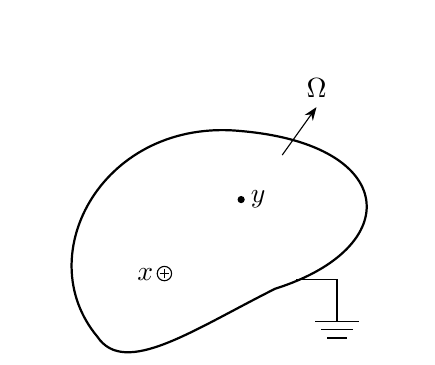
\begin{tikzpicture}[scale=.87,>=Stealth]
\draw[thick] (0,0) .. controls(-1,1.2) and(.1,3.2)..(2.1,3.0)
 .. controls(4.4,2.8) and(4.5,1.3)..(2.6,.7)
 .. controls(1.4,.1) and(.4,-.6)..(0,0);
\node at(.7,.9){$x$};\draw(.98,.92)circle(.105);\draw(.91,.92)--(1.05,.92);\draw(.98,.85)--(.98,.99);
\fill(2.1,2.0)circle(1.5pt) node[right]{$y$};
\draw[->](2.7,2.65)--(3.2,3.35)node[above]{$\Omega$};
\draw(2.9,.83)--(3.5,.83)--(3.5,.22);
\draw(3.18,.22)--(3.82,.22);
\draw(3.27,.10)--(3.73,.10);
\draw(3.36,-.02)--(3.64,-.02);
\end{tikzpicture}
\end{center}
\[
u=u(x)=u(x_1,\ldots,x_n),\qquad x\in\Omega.
\]
\[
\begin{cases}
-\Delta u=0,&x\in\Omega,\\
u=g(x),&x\in\partial\Omega,
\end{cases}
\qquad g\in C(\partial\Omega).
\]
\textbf{板书旁记：}\quad $Ax=y$。

\subsection*{多重指标记号}
\source{06}
\[
\alpha=(\alpha_1,\alpha_2,\ldots,\alpha_n),\qquad
|\alpha|=\alpha_1+\alpha_2+\cdots+\alpha_n,
\]
\[
D^\alpha u=
\frac{\partial^{|\alpha|}u}
{\partial x_1^{\alpha_1}\partial x_2^{\alpha_2}\cdots\partial x_n^{\alpha_n}}.
\]

\newpage
\section*{Hölder 空间}
\source{07、08；09 中重复部分合并于此}
设 $U\subset\R^n$ 开，$0<\gamma\leq1$，$u:U\to\R$。记
\[
\hn{u}=\sup_{\substack{x,y\in U\\x\ne y}}
\frac{|u(x)-u(y)|}{|x-y|^\gamma}.
\]
若 $\hn{u}<\infty$，则称 $u$ 是指数为 $\gamma$ 之 Hölder 连续函数。

\subsection*{定义}
设 $U\subset\R^n$ 开，$k\geq0$ 为整数，$0<\gamma\leq1$。定义
\[
\begin{aligned}
C^{k,\gamma}(\Ub)=\bigl\{u\in C^k(\Ub)\bigm|{}&
\text{对任意 }\alpha:\ |\alpha|\leq k,
\ D^\alpha u\text{ 在 }U\text{ 上有界},\\
&\text{且对任意 }\alpha:\ |\alpha|=k,
\ \hn{D^\alpha u}<\infty\bigr\}.
\end{aligned}
\]
设 $u\in C^{k,\gamma}(\Ub)$，令
\[
\boxed{
\|u\|_{C^{k,\gamma}(\Ub)}
=\sum_{|\alpha|\leq k}\|D^\alpha u\|_{C(\Ub)}
+\sum_{|\alpha|=k}\hn{D^\alpha u}.
}
\]
其中
\[
\|D^\alpha u\|_{C(\Ub)}=\sup_{x\in U}|D^\alpha u(x)|.
\]

\subsection*{定理}
\[
\left(C^{k,\gamma}(\Ub),\ \|\cdot\|_{C^{k,\gamma}(\Ub)}\right)
\quad\text{是 Banach 空间。}
\]

\subsection*{证明：$1^\circ$}
设 $\{u_m\}_{m=1}^\infty$ 是 $C^{k,\gamma}(\Ub)$ 中之 Cauchy 列。
则对每个 $\alpha:\ |\alpha|\leq k$，
\[
\{D^\alpha u_m\}_{m=1}^\infty
\quad\text{是 }C(\Ub)\text{ 中之 Cauchy 列。}
\]
于是
\[
D^\alpha u_m\longrightarrow u_\alpha\qquad\text{于 }C(\Ub).
\]
特别地，$\alpha=0$ 时，
\[
u_m\longrightarrow u_{(0,0,\ldots,0)}\triangleq u.
\]

\newpage
\subsection*{证明（续）：$2^\circ$}
\source{09、10、11；相同推导只保留一次}
下证 $D^\alpha u=u_\alpha$。示例性证明
\[
\frac{\partial u}{\partial x_1}=u_{(1,0,0,\ldots,0)}.
\]
\[
\begin{aligned}
&u_m(x_1+h,x_2,\ldots,x_n)-u_m(x_1,x_2,\ldots,x_n)\\
&\qquad=\int_{x_1}^{x_1+h}
\frac{\partial u_m}{\partial x_1}(\xi_1,x_2,\ldots,x_n)\dd\xi_1.
\end{aligned}
\]
\[
\frac{u(x_1+h,x_2,\ldots,x_n)-u(x_1,x_2,\ldots,x_n)}{h}.
\]
\ednote{照片中的差商写到此处，未接等式。上面积分取 $h$ 足够小，使积分线段留在 $U$ 内；此说明用于明确公式的适用范围。}

\subsection*{$3^\circ$}
任给 $\alpha:\ |\alpha|=k$，下证 $D^\alpha u$ 是 Hölder 连续的，且
\[
\hn{D^\alpha u_m-D^\alpha u}\longrightarrow0.
\]
\[
\forall\varepsilon>0,\quad\exists N\in\N,\quad
\text{s.t. }\forall m,l>N,\quad
\hn{D^\alpha u_m-D^\alpha u_l}<\varepsilon.
\]
即 $\forall x,y\in U$ 且 $x\ne y$，有
\[
\frac{\left|D^\alpha u_m(x)-D^\alpha u_l(x)
-\bigl(D^\alpha u_m(y)-D^\alpha u_l(y)\bigr)\right|}
{|x-y|^\gamma}<\varepsilon.
\]
令 $l\to\infty$，则
\[
\hn{D^\alpha u_m-D^\alpha u}\leq\varepsilon.
\]

\newpage
\section*{Sobolev 空间}
\source{12、13；紧支集的定义与图示合并}
\subsection*{1. 弱导数：$C_c^\infty(U)$}
\[
\begin{aligned}
u\in C_c^\infty(U)\quad\Longleftrightarrow\quad
&u\in C^\infty(U)\text{ 且}\\
&\operatorname{spt}u
=\overline{\{x\in U\mid u(x)\ne0\}}
\text{ 紧含于 }U.
\end{aligned}
\]
\begin{center}
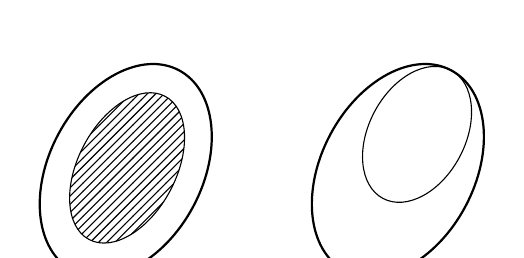
\begin{tikzpicture}[scale=.72]
\begin{scope}[rotate=-28]
\draw[thick](0,0)ellipse(1.35 and 2.0);
\draw[pattern=north east lines](0,.05)ellipse(.86 and 1.43);
\end{scope}
\begin{scope}[shift={(4.8,0)},rotate=-28]
\draw[thick](0,0)ellipse(1.35 and 2.0);
\draw(0,.72)ellipse(.85 and 1.28);
\end{scope}
\end{tikzpicture}
\end{center}
\ednote{两幅包含关系示意图依照板书重绘；原图没有文字标签，故不另添标签。}

设 $u\in C^1(\Ub)$。对任意 $\phi\in C_c^\infty(U)$，
\[
-\int_Uu\phi_{x_i}\dd x
=-\int_U\bigl((u\phi)_{x_i}-u_{x_i}\phi\bigr)\dd x.
\]
\ednote{9 月 7 日照片中的弱导数部分到以上等式为止；后续推导与正式定义见 9 月 9 日笔记。}

\clearpage
\fancyhead[R]{\small 2026 年 9 月 9 日}
\section*{2026 年 9 月 9 日：Sobolev 空间（续）}
\addcontentsline{toc}{section}{2026 年 9 月 9 日：Sobolev 空间（续）}
\source{9.9/01}
\subsection*{1. 弱导数：分部积分（接上次课）}
设 $u\in C^1(\Ub)$，$\phi\in C_c^\infty(U)$。接上次课的积分等式，
\[
\begin{aligned}
-\int_U(u\phi)_{x_i}\dd x+\int_Uu_{x_i}\phi\dd x
&=-\int_{\partial U}u\phi\cos(\vec n,x_i)\dd S
  +\int_Uu_{x_i}\phi\dd x\\
&=\int_Uu_{x_i}\phi\dd x.
\end{aligned}
\]
\ednote{保留板书的方向余弦记号 $\cos(\vec n,x_i)$，即外单位法向的第 $i$ 个分量。边界积分按板书的光滑边界情形理解；因 $\phi$ 紧支于 $U$，边界项为零。}

\subsection*{板书旁记：平面上的积分公式}
\[
P=P(x,y).
\]
\[
\begin{aligned}
\iint_D P_x\dd x\dd y
&=\int_{\partial D}0\dd x+P\dd y\\
&=\int_{\partial D}P\cos(\vec s,y)\dd s\\
&=\int_{\partial D}P\cos(\vec n,x)\dd s.
\end{aligned}
\]
\begin{center}
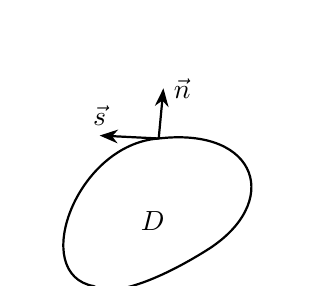
\begin{tikzpicture}[scale=.75,>=Stealth]
\draw[thick] (0,0) .. controls(-1.1,.2) and(-.3,2.4)..(1.1,2.5)
 .. controls(2.8,2.7) and(3.2,1.4)..(1.9,.6)
 .. controls(1.1,.1) and(.3,-.2)..(0,0);
\node at(1,1.1){$D$};
\draw[->,thick](1.1,2.5)--(.1,2.55)node[above]{$\vec s$};
\draw[->,thick](1.1,2.5)--(1.18,3.35)node[right]{$\vec n$};
\end{tikzpicture}
\end{center}

\subsection*{高阶情形}
\source{9.9/02}
设 $u\in C^k(\Ub)$，$\alpha$ 为多重指标，$|\alpha|\leq k$。则
\[
(-1)^{|\alpha|}\int_UuD^\alpha\phi\dd x
=\int_UD^\alpha u\,\phi\dd x,
\qquad\forall\phi\in C_c^\infty(U).
\]
\ednote{补明 $|\alpha|\leq k$，以保证上式中的经典导数存在。}

\newpage
\subsection*{弱导数的定义与唯一性}
\source{9.9/02；03 右侧的重复内容合并}
\textbf{定义。}设 $u,v\in L^1_{\mathrm{loc}}(U)$，$\alpha$ 是多重指标。若
\[
(-1)^{|\alpha|}\int_UuD^\alpha\phi\dd x
=\int_Uv\phi\dd x,
\qquad\forall\phi\in C_c^\infty(U),
\]
则称 $v$ 是 $u$ 的 $\alpha$ 阶弱导数，记为 $v=D^\alpha u$。

\textbf{唯一性。}设 $u$ 存在 $\alpha$ 阶弱导数，则该弱导数是唯一的。
\ednote{这里的唯一性指几乎处处相等意义下的唯一性。}

\textbf{证明。}设 $v_1,v_2\in L^1_{\mathrm{loc}}(U)$ 均为 $u$ 的 $\alpha$ 阶弱导数，则
\[
\int_U(v_1-v_2)\phi\dd x=0,
\qquad\forall\phi\in C_c^\infty(U).
\]
\textbf{板书所用结论：}设 $f\in L^1_{\mathrm{loc}}(U)$，若
\[
\int_Uf\phi\dd x=0,\qquad\forall\phi\in C_c^\infty(U),
\]
则 $f=0$ a.e. 于 $U$。

\subsection*{例 1}
\source{9.9/03}
设 $U=(0,2)$，
\[
u(x)=\begin{cases}
x,&0<x<1,\\
1,&1\leq x<2.
\end{cases}
\]
对任意 $\phi\in C_c^\infty(U)$，
\[
\begin{aligned}
-\int_Uu\phi'\dd x
&=-\int_0^1x\phi'\dd x-\int_1^2 1\phi'\dd x\\
&=-\left(\phi(1)-\int_0^1\phi\dd x\right)
  -\bigl(\phi(2)-\phi(1)\bigr)\\
&=\int_0^1\phi\dd x
=\int_Uv\phi\dd x,
\end{aligned}
\]
其中
\[
v(x)=\begin{cases}
1,&0<x<1,\\
0,&1\leq x<2.
\end{cases}
\]

\newpage
\subsection*{例 2}
\source{补充手写照片 1、2}
设 $U=(0,2)$，
\[
u(x)=\begin{cases}
x,&0<x<1,\\
2,&1\leq x<2.
\end{cases}
\]
\textbf{证明。}假设存在 $v\in L^1_{\mathrm{loc}}(U)$，使得
\[
-\int_Uu\phi'\dd x=\int_Uv\phi\dd x,
\qquad\forall\phi\in C_c^\infty(U).
\]
分部积分得
\[
-\int_0^1x\phi'\dd x-\int_1^2 2\phi'\dd x
=\phi(1)+\int_0^1\phi\dd x
=\int_0^2v\phi\dd x.
\]
取 $\phi_m\in C_c^\infty(U)$，满足
\[
0\leq\phi_m\leq1,\qquad\phi_m(1)=1,
\]
且当 $x\ne1$ 时，$\phi_m(x)\to0$（$m\to\infty$）。
\begin{center}
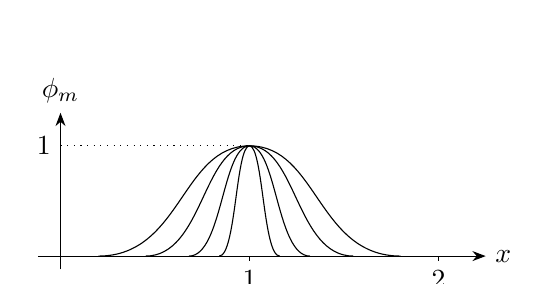
\begin{tikzpicture}[x=2.4cm,y=1.4cm]
\draw[-{Stealth}](-.12,0)--(2.25,0)node[right]{$x$};
\draw[-{Stealth}](0,-.12)--(0,1.3)node[above]{$\phi_m$};
\foreach \w in {.8,.55,.32,.16}{
\draw (1-\w,0)..controls(1-.45*\w,0)and(1-.45*\w,1)..(1,1)
..controls(1+.45*\w,1)and(1+.45*\w,0)..(1+\w,0);}
\draw[dotted](0,1)--(1,1);\node[left]at(0,1){$1$};
\foreach \x in {1,2}{\draw(\x,0)--(\x,-.04);\node[below]at(\x,-.04){$\x$};}
\end{tikzpicture}
\end{center}
代入上式，对任意 $m\in\N$，
\[
\phi_m(1)+\int_0^1\phi_m\dd x=\int_0^2v\phi_m\dd x.
\]
令 $m\to\infty$，得到
\[
1+0=0,
\]
矛盾。因此 $u$ 不存在属于 $L^1_{\mathrm{loc}}(U)$ 的弱导数。
\ednote{按图中支撑向 $1$ 收缩的方式选取 $\phi_m$，可使所有支撑包含在固定紧区间
$[\tfrac12,\tfrac32]\Subset U$ 中。由 $v$ 的局部可积性及控制收敛定理，右端积分趋于零。
照片末尾的一维绝对连续性注记已在下文保留，不再重复。}

\newpage
\subsection*{一维情形的注记}
\source{9.9/04、05}
设 $U=(a,b)$。
\[
\begin{gathered}
u\in L^1(a,b)\text{ 且 }u'\in L^1(a,b)\\
\Longleftrightarrow\\
u\text{ 有一个在 }[a,b]\text{ 上绝对连续的代表。}
\end{gathered}
\]
\ednote{板书右端写作“$u$ 是 $[a,b]$ 上绝对连续”。这里的 $u'$ 指弱导数，并将右端明确为“有绝对连续代表”，因为改变零测集上的函数值不改变弱导数。按板书的闭区间表述理解 $a,b$ 为有限端点。}

\subsection*{2. Sobolev 空间的定义}
设 $U\subset\R^n$ 开，$k\geq0$ 为整数，$1\leq p\leq\infty$。定义
\[
\begin{aligned}
W^{k,p}(U)=\bigl\{u\in L^p(U)\bigm|{}&
\text{对任意 }\alpha:\ |\alpha|\leq k,\\
&D^\alpha u\text{ 存在且 }D^\alpha u\in L^p(U)\bigr\}.
\end{aligned}
\]
当 $p=2$ 时，
\[
W^{k,2}(U)=H^k(U).
\]
\[
(u,v)=\int_U\sum_{|\alpha|\leq k}D^\alpha u\,D^\alpha v\dd x,
\qquad u,v\in H^k(U).
\]

\textbf{定义。}设 $u\in W^{k,p}(U)$，令
\[
\boxed{
\|u\|_{W^{k,p}(U)}=
\begin{cases}
\displaystyle\left(\sum_{|\alpha|\leq k}\int_U|D^\alpha u|^p\dd x\right)^{1/p},
&1\leq p<\infty,\\[12pt]
\displaystyle\sum_{|\alpha|\leq k}\operatorname*{ess\,sup}_{U}|D^\alpha u|,
&p=\infty.
\end{cases}}
\]
\ednote{照片 04 中范数尚未写完，采用照片 05 的完整版本；上述定义与范数仅录一次。}

\newpage
\subsection*{本质上确界}
\source{9.9/06}
\[
\operatorname*{ess\,sup}_{E}|f|
=\inf_{\substack{e\subset E\\|e|=0}}\ \sup_{x\in E\setminus e}|f(x)|
=\sup_{x\in E\setminus e_0}|f(x)|.
\]
\ednote{板书在末个等号处标有 $e_0\subset E$；此处 $e_0$ 亦为零测集。}

\subsection*{Sobolev 空间中的收敛}
设 $\{u_m\}_{m=1}^\infty\subset W^{k,p}(U)$，$u\in W^{k,p}(U)$。
称
\[
u_m\longrightarrow u\quad\text{于 }W^{k,p}(U),
\]
若
\[
\|u_m-u\|_{W^{k,p}(U)}\longrightarrow0\qquad(m\to\infty).
\]
若对任意 $V\Subset U$，都有
\[
u_m\longrightarrow u\quad\text{于 }W^{k,p}(V),
\]
则称
\[
u_m\longrightarrow u\quad\text{于 }W^{k,p}_{\mathrm{loc}}(U).
\]
\ednote{照片把 $\mathrm{loc}$ 写在全域收敛的记号下方，而局部条件以黄色另补。这里按相应的范数条件分开整理：全域范数趋零对应 $W^{k,p}(U)$；每个 $V\Subset U$ 上范数趋零对应局部收敛。$V\Subset U$ 表示 $\overline V$ 紧且包含于 $U$。}

\subsection*{$W_0^{k,p}(U)$}
\textbf{定义。}记 $C_c^\infty(U)$ 在 $W^{k,p}(U)$ 中的闭包为 $W_0^{k,p}(U)$。
即
\[
\begin{aligned}
u\in W_0^{k,p}(U)\quad\Longleftrightarrow\quad
&\text{存在 }\{u_m\}_{m=1}^\infty\subset C_c^\infty(U),\\
&\text{s.t. }u_m\longrightarrow u\quad\text{于 }W^{k,p}(U).
\end{aligned}
\]

\newpage
\subsection*{例 3：$u(x)=|x|^{-\alpha}$}
\source{9.9/07、08；两图拼接为一次推导}
设 $U=B(0,1)$，
\[
u(x)=|x|^{-\alpha},\qquad x\in U,\quad x\ne0,\quad\alpha>0.
\]
问：对什么 $\alpha>0$、$n$、$p$，有 $u\in W^{1,p}(U)$？

\textbf{解。} $\alpha<n\Rightarrow u\in L^1(U)$。对 $x\ne0$，
\[
u_{x_i}=-\alpha|x|^{-\alpha-1}\frac{x_i}{|x|},
\qquad\alpha+1<n\Rightarrow u_{x_i}\in L^1(U).
\]
对任意 $\phi\in C_c^\infty(U)$，
\[
\begin{aligned}
-\int_Uu\phi_{x_i}\dd x
&=-\lim_{\varepsilon\to0}\int_{U\setminus B(0,\varepsilon)}u\phi_{x_i}\dd x\\
&=-\lim_{\varepsilon\to0}\int_{\partial(U\setminus B(0,\varepsilon))}
 u\phi\nu_i\dd S
 +\lim_{\varepsilon\to0}\int_{U\setminus B(0,\varepsilon)}u_{x_i}\phi\dd x\\
&=-\lim_{\varepsilon\to0}\int_{\partial B(0,\varepsilon)}u\phi\nu_i\dd S
 +\lim_{\varepsilon\to0}\int_{U\setminus B(0,\varepsilon)}u_{x_i}\phi\dd x\\
&=\int_Uu_{x_i}\phi\dd x.
\end{aligned}
\]
边界项的估计为
\[
\left|\int_{\partial B(0,\varepsilon)}u\phi\nu_i\dd S\right|
\leq C\varepsilon^{-\alpha}\,n|B(0,1)|\,\varepsilon^{n-1}.
\]
\ednote{$\nu$ 沿用挖去小球后区域的外法向：在内边界上指向球心。上述极限推导在 $\alpha+1<n$ 时进行，估计右端趋于零。}
\begin{center}
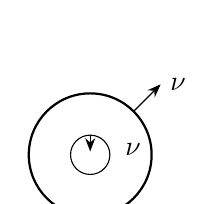
\begin{tikzpicture}[scale=.52,>=Stealth]
\draw[thick](0,0)circle(1.5);\draw(0,0)circle(.48);
\draw[->](1.06,1.06)--(1.72,1.72)node[right]{$\nu$};
\draw[->](0,.48)--(0,.08);\node[right]at(.62,.12){$\nu$};
\end{tikzpicture}
\end{center}
\[
Du=-\alpha|x|^{-\alpha-1}\frac{x}{|x|},\qquad
|Du|=\frac{\alpha}{|x|^{\alpha+1}}.
\]
\[
(\alpha+1)p<n\ \Longrightarrow\ |Du|\in L^p(U).
\]
\[
\boxed{u\in W^{1,p}(U)\quad\Longleftrightarrow\quad0<\alpha<\frac np-1.}
\]
\textbf{注。} $p=n\Rightarrow u\notin W^{1,p}(U)$；$p>n\Rightarrow u\notin W^{1,p}(U)$。
\ednote{保留板书“例 3”的编号；例 2 已依据后来提供的两张手写照片补入。上述含 $n/p$ 的条件按 $1\leq p<\infty$ 理解；$\alpha>0$ 时 $u$ 本身也不属于 $L^\infty(U)$。}

\newpage
\subsection*{板书续例：奇性函数的级数}
\source{9.9/09}
\[
u(x)=\sum_{k=1}^{\infty}\frac1{2^k}|x-r_k|^{-\alpha},\qquad x\in U,
\]
其中 $\alpha>0$。当
\[
0<\alpha<\frac np-1
\]
时，$u\in W^{1,p}(U)$。
\ednote{沿用前例的 $U=B(0,1)$。照片未写出点列 $\{r_k\}$ 的选取条件，故保留该记号，不补设稠密性等未拍到的条件。此处函数作为几乎处处定义的函数理解，奇点处不要求逐点取有限值。}

\subsection*{板书旁记：$L^p$ 中的级数收敛}
\[
\{f_k\}_{k=1}^{\infty}\subset L^p(U),\qquad
\sum_{k=1}^{\infty}\|f_k\|_{L^p(U)}\triangleq B<\infty.
\]
则
\[
\sum_{k=1}^{\infty}f_k\quad\text{于 }L^p(U)\text{ 中收敛。}
\]

\clearpage
\fancyhead[R]{\small 2026 年 9 月 14 日}
\section*{2026 年 9 月 14 日：基本性质与磨光}
\addcontentsline{toc}{section}{2026 年 9 月 14 日：基本性质与磨光}
\subsection*{3. 基本性质}
\source{9.14/01、02 左侧}
\textbf{定理。}设 $u,v\in W^{k,p}(U)$，$|\alpha|\leq k$。

\textbf{(i)} $D^\alpha u\in W^{k-|\alpha|,p}(U)$，且
\[
D^\alpha(D^\beta u)=D^\beta(D^\alpha u)=D^{\alpha+\beta}u,
\qquad |\alpha|+|\beta|\leq k.
\]
\textbf{(ii)} 设 $\lambda,\mu\in\R$，则 $\lambda u+\mu v\in W^{k,p}(U)$。

\textbf{(iii)} 设 $V\subset U$，则 $u\in W^{k,p}(V)$。

\textbf{(iv)} 设 $\zeta\in C_c^\infty(U)$，则 $\zeta u\in W^{k,p}(U)$，且
\[
\boxed{D^\alpha(\zeta u)=\sum_{\beta\leq\alpha}
\binom\alpha\beta D^\beta\zeta\,D^{\alpha-\beta}u.}
\]
其中
\[
\binom\alpha\beta=\frac{\alpha!}{\beta!(\alpha-\beta)!}.
\]
\ednote{(iii) 中 $V$ 取开集，$u$ 在 $V$ 上指其限制；多重指标的 $\beta\leq\alpha$ 按分量理解。}

\textbf{证明（板书给出 (iv) 的一阶情形）。}对任意 $\phi\in C_c^\infty(U)$，
\[
\begin{aligned}
-\int_U(\zeta u)\phi_{x_i}\dd x
&=-\int_Uu\bigl[(\zeta\phi)_{x_i}-\zeta_{x_i}\phi\bigr]\dd x\\
&=-\int_Uu(\zeta\phi)_{x_i}\dd x+\int_U(u\zeta_{x_i})\phi\dd x\\
&=\int_Uu_{x_i}\zeta\phi\dd x+\int_U(u\zeta_{x_i})\phi\dd x\\
&=\int_U(u_{x_i}\zeta+u\zeta_{x_i})\phi\dd x.
\end{aligned}
\]
\ednote{照片 02 将 $-\int_Uu(\zeta\phi)_{x_i}$ 划掉并在下方改写为 $\int_Uu_{x_i}\zeta\phi$；这里按老师的改写顺接。}

\newpage
\subsection*{完备性}
\source{9.14/02 右侧、03 上方}
\textbf{定理。}$W^{k,p}(U)$ 是 Banach 空间。

\textbf{证明。}设 $\{u_m\}_{m=1}^{\infty}\subset W^{k,p}(U)$ 是 Cauchy 列。
则对任意 $\alpha:\ |\alpha|\leq k$，$\{D^\alpha u_m\}$ 是 $L^p(U)$ 中的 Cauchy 列，故
\[
D^\alpha u_m\longrightarrow u_\alpha\quad\text{于 }L^p(U).
\]
特别地，$\alpha=0$ 时，
\[
u_m\longrightarrow u_{(0,0,\ldots,0)}\triangleq u\quad\text{于 }L^p(U).
\]
\[
(-1)^{|\alpha|}\int_Uu_mD^\alpha\phi\dd x
=\int_UD^\alpha u_m\,\phi\dd x,
\qquad\forall\phi\in C_c^\infty(U).
\]
\[
(-1)^{|\alpha|}\int_UuD^\alpha\phi\dd x
=\int_Uu_\alpha\phi\dd x,
\qquad\forall\phi\in C_c^\infty(U).
\]

\subsection*{卷积与磨光}
\source{9.14/03}
\textbf{定义。(i)} 令
\[
\eta(x)=\begin{cases}
\displaystyle C\exp\left(-\frac1{1-|x|^2}\right),&|x|<1,\\[5pt]
0,&|x|\geq1,
\end{cases}
\]
其中 $C>0$，使得
\[
\int_{\R^n}\eta(x)\dd x=1.
\]
则 $\eta\in C^\infty(\R^n)$，$\operatorname{spt}\eta=\overline{B(0,1)}$。

\textbf{(ii)} 对任意 $\varepsilon>0$，令
\[
\eta_\varepsilon(x)=\varepsilon^{-n}\eta\left(\frac{x}{\varepsilon}\right),
\qquad x\in\R^n.
\]
则
\[
\eta_\varepsilon\in C^\infty(\R^n),\qquad
\int_{\R^n}\eta_\varepsilon(x)\dd x=1,\qquad
\operatorname{spt}\eta_\varepsilon=\overline{B(0,\varepsilon)}.
\]

\newpage
\subsection*{磨光的定义与光滑性}
\source{9.14/04--07；05、06、07 的同一推导合并}
设 $U\subset\R^n$ 开，$\varepsilon>0$，记
\[
U_\varepsilon=\{x\in U\mid\operatorname{dist}(x,\partial U)>\varepsilon\}.
\]
\textbf{定义。}设 $f\in L^1_{\mathrm{loc}}(U)$，$f$ 的磨光定义为
\[
\begin{aligned}
f^\varepsilon(x)&=(\eta_\varepsilon*f)(x),\qquad x\in U_\varepsilon,\\
&=\int_U\eta_\varepsilon(x-y)f(y)\dd y\\
&=\int_{B(x,\varepsilon)}\eta_\varepsilon(x-y)f(y)\dd y\\
&=\int_{B(0,\varepsilon)}\eta_\varepsilon(z)f(x-z)\dd z.
\end{aligned}
\]
\begin{center}
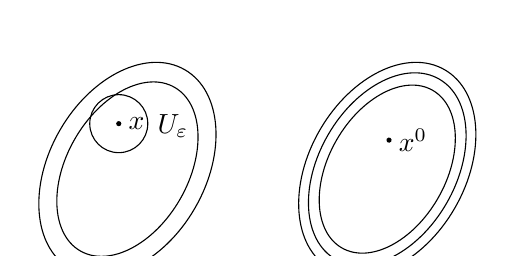
\begin{tikzpicture}[scale=.55]
\draw[rotate=-30](0,0)ellipse(1.8 and 2.65);
\draw[rotate=-30](0,0)ellipse(1.4 and 2.18);
\draw(-.2,1.05)circle(.67);\fill(-.2,1.05)circle(1.7pt);
\node[right]at(-.2,1.05){$x$};\node at(1.05,1.0){$U_\varepsilon$};
\begin{scope}[shift={(6,0)},rotate=-30]
\draw(0,0)ellipse(1.8 and 2.65);
\draw(0,0)ellipse(1.58 and 2.4);
\draw(0,0)ellipse(1.35 and 2.1);
\fill(-.3,.6)circle(1.7pt)node[right]{$x^0$};
\end{scope}
\end{tikzpicture}
\end{center}
\textbf{定理。(i)} $f^\varepsilon\in C^\infty(U_\varepsilon)$。

\textbf{证明。}任给 $x^0\in U_\varepsilon$，$e_i=(0,\ldots,1,\ldots,0)$。
取 $V\Subset U$，使对任意 $|h|<\frac12\operatorname{dist}(x^0,\partial U_\varepsilon)$，
\[
B(x^0+he_i,\varepsilon)\subset V.
\]
\[
\begin{aligned}
\frac{f^\varepsilon(x^0+he_i)-f^\varepsilon(x^0)}h
&=\int_U\frac{\eta_\varepsilon(x^0+he_i-y)-\eta_\varepsilon(x^0-y)}h f(y)\dd y\\
&=\int_V\frac{\eta_\varepsilon(x^0+he_i-y)-\eta_\varepsilon(x^0-y)}h f(y)\dd y\\
&=\int_V(\eta_\varepsilon)_{x_i}(x^0+\theta he_i-y)f(y)\dd y\\
&\xrightarrow{h\to0}\int_U(\eta_\varepsilon)_{x_i}(x^0-y)f(y)\dd y.
\end{aligned}
\]
\ednote{中值定理中的 $0<\theta<1$ 可依赖于 $h,y$。这里按照片保留一阶差商推导，未另加高阶证明。}

\newpage
\subsection*{磨光的收敛性质：几乎处处收敛}
\source{9.14/08}
\textbf{(ii)} $f^\varepsilon\to f$ a.e. 于 $U$（$\varepsilon\to0$）。

\textbf{证明。}由 Lebesgue 微分定理，
\[
\lim_{\varepsilon\to0}\frac1{|B(x,\varepsilon)|}
\int_{B(x,\varepsilon)}|f(y)-f(x)|\dd y=0
\quad\text{a.e. 于 }U.
\]
对上述收敛之 $x$，有
\[
\begin{aligned}
|f^\varepsilon(x)-f(x)|
&=\left|\int_{B(x,\varepsilon)}\eta_\varepsilon(x-y)f(y)\dd y
-\int_{B(x,\varepsilon)}\eta_\varepsilon(x-y)f(x)\dd y\right|\\
&\leq\int_{B(x,\varepsilon)}\eta_\varepsilon(x-y)|f(y)-f(x)|\dd y\\
&\leq\frac{|B(0,1)|C}{|B(0,1)|\varepsilon^n}
\int_{B(x,\varepsilon)}|f(y)-f(x)|\dd y\\
&\leq\frac C{|B(x,\varepsilon)|}
\int_{B(x,\varepsilon)}|f(y)-f(x)|\dd y\longrightarrow0.
\end{aligned}
\]
其中 $\eta_\varepsilon(x-y)=\varepsilon^{-n}\eta((x-y)/\varepsilon)$。
\ednote{估计中的 $C$ 按板书作一般常数使用，最后一步可吸收 $|B(0,1)|$。}

\subsection*{连续函数的局部一致收敛}
\source{9.14/09}
\textbf{(iii)} 设 $f\in C(U)$，则 $f^\varepsilon\to f$ 于 $C_{\mathrm{loc}}(U)$，
即对任意 $V\Subset U$，$f^\varepsilon\to f$ 一致地于 $V$。

\textbf{证明。}任给 $V\Subset U$，取 $W$ 使得 $V\Subset W\Subset U$。
因 $f\in C(\overline W)$，对任意 $\delta>0$，存在 $\eta>0$，使
\[
\forall x,y\in W,\quad |x-y|<\eta\quad\Longrightarrow\quad|f(y)-f(x)|<\delta.
\]
因此当 $\varepsilon<\min\{\eta,\operatorname{dist}(V,\partial W)\}$ 时，对任意 $x\in V$，
\[
\frac1{|B(x,\varepsilon)|}\int_{B(x,\varepsilon)}|f(y)-f(x)|\dd y<\delta.
\]
\ednote{此处 $\eta>0$ 是板书中一致连续性的距离参数，与磨光核的函数记号同形。结合上面的估计即可得到局部一致收敛。}

\newpage
\subsection*{局部 $L^p$ 收敛}
\source{9.14/10--12；重复的逼近估计合并}
\textbf{(iv)} 设 $1\leq p<\infty$，$f\in L^p_{\mathrm{loc}}(U)$，则
\[
f^\varepsilon\longrightarrow f\quad\text{于 }L^p_{\mathrm{loc}}(U),
\]
即对任意 $V\Subset U$，$f^\varepsilon\to f$ 于 $L^p(V)$。

\textbf{证明。}任给 $V\Subset U$，取 $W$ 使得 $V\Subset W\Subset U$。
于是 $f\in L^p(W)$。对任意 $\delta>0$，存在 $g\in C_c(W)$，使得
\[
\|f-g\|_{L^p(W)}<\delta.
\]
\[
\begin{aligned}
\|f^\varepsilon-f\|_{L^p(V)}
&\leq\|f^\varepsilon-g^\varepsilon\|_{L^p(V)}
+\|g^\varepsilon-g\|_{L^p(V)}+\|g-f\|_{L^p(V)}\\
&\leq\|f^\varepsilon-g^\varepsilon\|_{L^p(V)}
+\|g^\varepsilon-g\|_{L^p(V)}+\|g-f\|_{L^p(W)}.
\end{aligned}
\]
\ednote{照片 10、12 的三角不等式第一行漏写 $\|g-f\|$，而后面又使用了该项；此处补齐。}
板书所用估计为
\[
\boxed{\|f^\varepsilon\|_{L^p(V)}\leq\|f\|_{L^p(W)},
\qquad\varepsilon<\operatorname{dist}(V,\partial W).}
\]
因而第一项 $<\delta$，第三项 $<\delta$。又由 (iii)，第二项趋于零，故
\[
\limsup_{\varepsilon\to0}\|f^\varepsilon-f\|_{L^p(V)}\leq2\delta.
\]

\subsection*{板书旁记：Hölder 不等式}
\source{9.14/11 右侧}
设 $1\leq p,q\leq\infty$，$\frac1p+\frac1q=1$。
若 $f\in L^p(E)$，$g\in L^q(E)$，则 $fg\in L^1(E)$，且
\[
\|fg\|_{L^1(E)}\leq\|f\|_{L^p(E)}\|g\|_{L^q(E)}.
\]
板书所取的共轭指数：$p$，$p/(p-1)$。

\newpage
\subsection*{上述范数估计的证明}
\source{9.14/11 左侧、12 左侧}
对任意 $x\in V$，
\[
\begin{aligned}
|f^\varepsilon(x)|
&=\left|\int_{B(x,\varepsilon)}\eta_\varepsilon(x-y)f(y)\dd y\right|\\
&\leq\int_{B(x,\varepsilon)}[\eta_\varepsilon(x-y)]^{1/p}|f(y)|
[\eta_\varepsilon(x-y)]^{(p-1)/p}\dd y\\
&\leq\left(\int_{B(x,\varepsilon)}\eta_\varepsilon(x-y)|f(y)|^p\dd y\right)^{1/p}.
\end{aligned}
\]
\ednote{上述 Hölder 分解适用于 $p>1$；当 $p=1$ 时，直接用积分的三角不等式得到相同估计。}
当 $\varepsilon<\operatorname{dist}(V,\partial W)$ 时，对任意 $x\in V$，
\[
\begin{aligned}
|f^\varepsilon(x)|^p
&\leq\int_{B(x,\varepsilon)}\eta_\varepsilon(x-y)|f(y)|^p\dd y\\
&\leq\int_W\eta_\varepsilon(x-y)|f(y)|^p\dd y.
\end{aligned}
\]
\[
\begin{aligned}
\int_V|f^\varepsilon(x)|^p\dd x
&\leq\int_W\int_V\eta_\varepsilon(x-y)|f(y)|^p\dd x\dd y\\
&\leq\int_W|f(y)|^p\dd y.
\end{aligned}
\]
故 $\|f^\varepsilon\|_{L^p(V)}\leq\|f\|_{L^p(W)}$。

\clearpage
\fancyhead[R]{\small 2026 年 9 月 16 日}
\begin{center}
{\LARGE\bfseries 9 月 16 日课堂板书}\\[4pt]
{逼近、边界光滑性与局部展平}
\end{center}
\section{逼近}
\subsection{内部逼近}
\source{9.16/01、02 左侧}
\textbf{定理。}设 $U\subset\R^n$ 为开集，$k\geq1$ 为整数，$1\leq p<\infty$，
$u\in W^{k,p}(U)$。令
\[
U_\varepsilon=\{x\in U:\operatorname{dist}(x,\partial U)>\varepsilon\},
\qquad u^\varepsilon=\eta_\varepsilon*u\quad\text{于 }U_\varepsilon.
\]
则对 $|\alpha|\leq k$，
\[
\boxed{D^\alpha u^\varepsilon=\eta_\varepsilon*D^\alpha u\quad\text{于 }U_\varepsilon,}
\qquad
u^\varepsilon\longrightarrow u\quad\text{于 }W_{\mathrm{loc}}^{k,p}(U).
\]
\textbf{证明。}对 $x\in U_\varepsilon$，
\[
\begin{aligned}
D^\alpha u^\varepsilon(x)
&=D^\alpha\int_U\eta_\varepsilon(x-y)u(y)\dd y\\
&=\int_U D_x^\alpha\eta_\varepsilon(x-y)u(y)\dd y\\
&=(-1)^{|\alpha|}\int_U u(y)D_y^\alpha[\eta_\varepsilon(x-y)]\dd y\\
&=\int_U\eta_\varepsilon(x-y)D^\alpha u(y)\dd y.
\end{aligned}
\]
对任意 $V\Subset U$，由局部 $L^p$ 逼近，
\[
D^\alpha u^\varepsilon=\eta_\varepsilon*D^\alpha u
\longrightarrow D^\alpha u\quad\text{于 }L^p(V),\qquad |\alpha|\leq k.
\]
\subsection{整体逼近}
\source{9.16/02 右侧}
\textbf{定理。}设 $U\subset\R^n$ 为有界开集，$1\leq p<\infty$，
$u\in W^{k,p}(U)$。则存在
\[
\{u_m\}\subset C^\infty(U)\cap W^{k,p}(U),\qquad
u_m\longrightarrow u\quad\text{于 }W^{k,p}(U).
\]
即：任给 $\delta>0$，找到 $v\in C^\infty(U)\cap W^{k,p}(U)$，使
\[
\|v-u\|_{W^{k,p}(U)}<\delta.
\]

\newpage
\subsection*{整体逼近的证明：开集分层与单位分解}
\source{9.16/02 右侧、03、04}
令
\[
U_i=\left\{x\in U:\operatorname{dist}(x,\partial U)>\frac1i\right\},
\quad i=1,2,\ldots,\qquad U_0=U_{-1}=\varnothing,
\]
\[
V_i=U_{i+1}\setminus\overline{U_{i-1}}.
\]
则 $V_i\Subset U$，且 $U=\bigcup_{i=1}^\infty V_i$。
\begin{center}
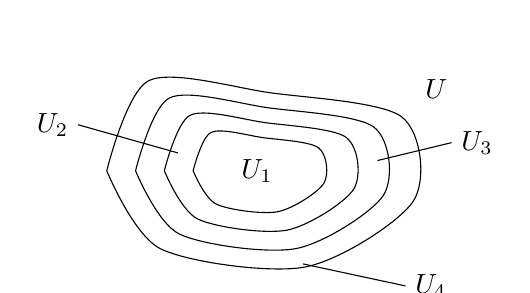
\begin{tikzpicture}[scale=.65]
\foreach \s/\lab in {1/U_1,1.45/U_2,1.9/U_3,2.35/U_4} {
\draw[smooth] plot coordinates {(-1.25*\s,0) (-.9*\s,.75*\s) (.1*\s,.65*\s) (1.2*\s,.45*\s) (1.3*\s,-.25*\s) (.4*\s,-.8*\s) (-.8*\s,-.65*\s) (-1.25*\s,0)};
}
\node at (0,0) {$U_1$};
\draw (-1.55,.35)--(-3.5,.9) node[left]{$U_2$};
\draw (2.35,.2)--(3.8,.55) node[right]{$U_3$};
\draw (.9,-1.82)--(2.9,-2.25) node[right]{$U_4$};
\node at (3.5,1.6) {$U$};
\end{tikzpicture}
\end{center}
取相应的 $C^\infty$ 单位分解：
\[
\zeta_i\in C_c^\infty(V_i),\qquad 0\leq\zeta_i\leq1,
\qquad\sum_{i=1}^\infty\zeta_i=1\quad\text{于 }U.
\]
因此
\[
u=\sum_{i=1}^\infty u\zeta_i,\qquad
u\zeta_i\in W^{k,p}(U),\qquad\operatorname{supp}(u\zeta_i)\subset V_i.
\]
再令
\[
W_i=U_{i+2}\setminus\overline{U_{i-2}},\qquad i\geq1,
\qquad V_i\Subset W_i\Subset U.
\]
任给 $\delta>0$，取充分小的 $\varepsilon_i>0$，使得
\[
u^i=\eta_{\varepsilon_i}*(u\zeta_i)\in C^\infty(U),\qquad
\operatorname{supp}u^i\subset W_i,
\]
\[
\|u^i-u\zeta_i\|_{W^{k,p}(U)}
=\|u^i-u\zeta_i\|_{W^{k,p}(W_i)}<\frac{\delta}{2^i}.
\]
\ednote{这里将紧支撑的 $u\zeta_i$ 在 $U$ 外延拓为零后作卷积。}

\newpage
\subsection*{整体逼近的证明（续）}
\source{9.16/04--06；重复推导合并}
令
\[
v=\sum_{i=1}^\infty u^i\in C^\infty(U).
\]
对任意 $V\Subset U$，
\[
\begin{aligned}
\|v-u\|_{W^{k,p}(V)}
&=\left\|\sum_{i=1}^\infty u^i-\sum_{i=1}^\infty u\zeta_i\right\|_{W^{k,p}(V)}\\
&\leq\sum_{i=1}^\infty\|u^i-u\zeta_i\|_{W^{k,p}(U)}<\delta.
\end{aligned}
\]
\ednote{上述和在 $U$ 内局部有限，故 $v$ 光滑。令 $V$ 递增穷尽 $U$，即得
$\|v-u\|_{W^{k,p}(U)}\leq\sum_i\|u^i-u\zeta_i\|_{W^{k,p}(U)}<\delta$。}

\subsection*{注：$p=\infty$ 的情形}
\source{9.16/07}
取
\[
u(x)=|x|,\quad x\in(-1,1),\qquad
u'(x)=\frac{x}{|x|}\quad(x\ne0).
\]
则 $u\in W^{1,\infty}(-1,1)$。当 $\delta$ 充分小时，不存在
$v\in C^\infty(-1,1)\cap W^{1,\infty}(-1,1)$ 使
\[
\|v-u\|_{W^{1,\infty}(-1,1)}<\delta.
\]
否则，$\|v'-u'\|_{L^\infty(-1,1)}<\delta$，即除去一个零测集 $e$ 后，
\[
\sup_{x\in(-1,1)\setminus e}|v'(x)-u'(x)|<\delta.
\]
\begin{center}
\begin{tikzpicture}[x=3cm,y=1cm]
\draw[-{Stealth}] (-1.15,0)--(1.2,0);
\foreach \x in {-1,0,1}{\draw (\x,-.06)--(\x,.06);\node[below] at(\x,-.07){$\x$};}
\draw[-{Stealth}](-.7,.35)--(-.15,.35) node[midway,above]{$\hat x_m$};
\draw[-{Stealth}](.7,.35)--(.15,.35) node[midway,above]{$x_m$};
\end{tikzpicture}
\end{center}
取 $x_m\downarrow0$，$\hat x_m\uparrow0$，则
\[
v'(x_m)>1-\delta,\qquad v'(\hat x_m)<-1+\delta.
\]
\ednote{两列点均取在 $e$ 外。由 $v'$ 在 $0$ 处连续，得到
$1-\delta\leq v'(0)\leq-1+\delta$，当 $\delta<1$ 时矛盾。
$u'$ 是弱导数，其在单点 $0$ 的取值不影响上述结论。}

\newpage
\subsection{直到边界的整体逼近}
\source{9.16/08、09、14（手写补充）}
考虑开集与函数
\[
U=\{(x,y):0<|x|<1,\ 0<y<1\},\qquad
u(x,y)=\begin{cases}
1,&0<x<1,\ 0<y<1,\\
0,&-1<x<0,\ 0<y<1.
\end{cases}
\]
\begin{center}
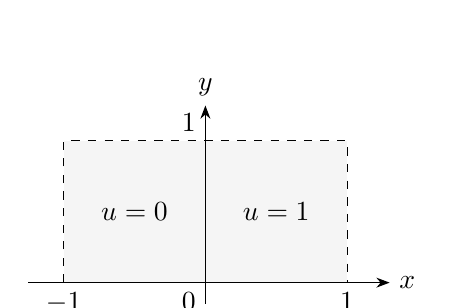
\begin{tikzpicture}[scale=1.8]
\fill[gray!8](-1,0) rectangle (1,1);
\draw[dashed](-1,0) rectangle(1,1);\draw[dashed](0,0)--(0,1);
\draw[-{Stealth}](-1.25,0)--(1.3,0) node[right]{$x$};
\draw[-{Stealth}](0,-.15)--(0,1.25) node[above]{$y$};
\node at(-.5,.5){$u=0$};\node at(.5,.5){$u=1$};
\node[below] at(-1,0){$-1$};\node[below left] at(0,0){$0$};
\node[below] at(1,0){$1$};\node[above left] at(0,1){$1$};
\end{tikzpicture}
\end{center}
有 $u\in W^{1,p}(U)$。设 $1\leq p<\infty$，假设当 $\delta>0$ 充分小时，存在
$v\in C^\infty(\overline U)$ 使
\[
\|v-u\|_{W^{1,p}(U)}<\delta.
\]
在右侧矩形上，
\[
\begin{aligned}
\int_0^1\!\int_0^1(u-v)\dd y\dd x
&\leq\int_0^1\!\int_0^1|u-v|\dd y\dd x\\
&\leq\left(\int_0^1\!\int_0^1|u-v|^p\dd y\dd x\right)^{1/p}\\
&\leq\left(\iint_U|u-v|^p\dd x\dd y\right)^{1/p}<\delta.
\end{aligned}
\]
因此 $\displaystyle\int_0^1\!\int_0^1v(x,y)\dd y\dd x>1-\delta$。
在左侧矩形上，
\[
\int_{-1}^0\!\int_0^1(v-u)\dd y\dd x<\delta,
\qquad\int_{-1}^0\!\int_0^1v(x,y)\dd y\dd x<\delta.
\]
于是存在 $b\in(0,1)$、$a\in(-1,0)$，使得
\[
\int_0^1v(b,y)\dd y>1-\delta,\qquad
\int_0^1v(a,y)\dd y<\delta.
\]

\newpage
\subsection*{反例的推导（续）}
\source{9.16/10 左侧}
\[
\begin{aligned}
1-2\delta
&<\int_0^1v(b,y)\dd y-\int_0^1v(a,y)\dd y\\
&\leq\int_0^1\!\int_{-1}^1|Dv|\dd x\dd y
=\iint_U|Dv|\dd x\dd y\\
&\leq 2^{1-1/p}\left(\iint_U|Dv|^p\dd x\dd y\right)^{1/p}\\
&=2^{1-1/p}\|Dv-Du\|_{L^p(U)}<2^{1-1/p}\delta.
\end{aligned}
\]
\ednote{$Du=0$ 于 $U$。因此当 $\delta<(2+2^{1-1/p})^{-1}$ 时矛盾。
此处的 $C^\infty(\overline U)$ 要求跨过裂缝 $x=0$ 后仍光滑，故可用微积分基本定理。}

\section{边界光滑性}
\source{9.16/11；13 右侧的圆形示意图合并于此}
\textbf{定义。}设 $U\subset\R^n$ 为有界开集。称 $\partial U$ 为 $C^k$ 的，
如果对任意 $x^0\in\partial U$，存在 $r>0$ 以及 $C^k$ 函数
$\gamma:\R^{n-1}\to\R$，使得（适当选取坐标后）
\[
U\cap B(x^0,r)=\{x\in B(x^0,r):x_n>\gamma(x_1,\ldots,x_{n-1})\}.
\]
\ednote{补出“适当选取坐标后”：每个边界点附近允许作刚性坐标变换，使区域在图像的上方。}
\begin{center}
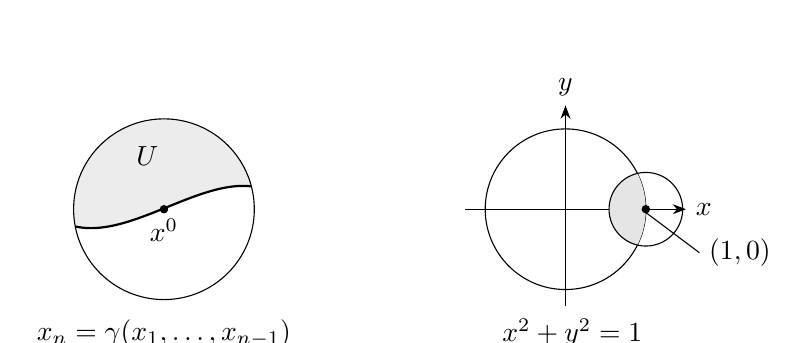
\begin{tikzpicture}[scale=.85]
\begin{scope}
\clip(0,0) circle(1.35);
\fill[gray!15](-1.5,-.2) .. controls(-.6,-.6) and(.6,.6)..(1.5,.3)--(1.5,1.6)--(-1.5,1.6)--cycle;
\draw[thick](-1.5,-.2)..controls(-.6,-.6) and(.6,.6)..(1.5,.3);
\end{scope}
\draw(0,0)circle(1.35);\fill(0,0)circle(1.8pt);
\node[below]at(0,0){$x^0$};\node at(-.25,.8){$U$};
\node[below]at(0,-1.5){$x_n=\gamma(x_1,\ldots,x_{n-1})$};
\begin{scope}[xshift=6cm]
\draw[-{Stealth}](-1.5,0)--(1.8,0)node[right]{$x$};
\draw[-{Stealth}](0,-1.45)--(0,1.55)node[above]{$y$};
\draw(0,0)circle(1.2);
\begin{scope}\clip(1.2,0)circle(.55);\fill[gray!20](0,0)circle(1.2);\end{scope}
\draw(1.2,0)circle(.55);\fill(1.2,0)circle(1.8pt);
\draw(1.2,-.05)--(2,-.65) node[right]{$(1,0)$};
\node[below]at(.1,-1.5){$x^2+y^2=1$};
\end{scope}
\end{tikzpicture}
\end{center}
圆周的例子：在 $(1,0)$ 附近，边界为 $x=\sqrt{1-y^2}$，圆盘内部为
$x<\sqrt{1-y^2}$。

\newpage
\subsection{边界的局部展平}
\source{9.16/12、13 左侧}
令 $\Phi=(\Phi^1,\ldots,\Phi^n):\R^n\to\R^n$，其中
\[
\begin{cases}
y_1=x_1=\Phi^1(x),\\
\hspace{10mm}\vdots\\
y_{n-1}=x_{n-1}=\Phi^{n-1}(x),\\
y_n=x_n-\gamma(x_1,\ldots,x_{n-1})=\Phi^n(x).
\end{cases}
\]
记 $D=\Phi(B(x^0,r))$，则
\[
\Phi(U\cap B(x^0,r))=\{y\in D:y_n>0\},
\]
\[
\Phi(\partial U\cap B(x^0,r))=\{y\in D:y_n=0\}.
\]
\begin{center}
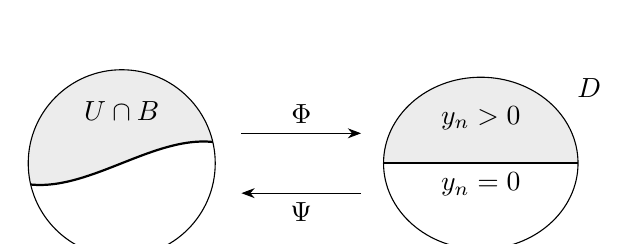
\begin{tikzpicture}[scale=.95]
\begin{scope}
\clip(0,0)circle(1.25);
\fill[gray!15](-1.4,-.25)..controls(-.5,-.5)and(.5,.5)..(1.4,.25)--(1.4,1.4)--(-1.4,1.4)--cycle;
\draw[thick](-1.4,-.25)..controls(-.5,-.5)and(.5,.5)..(1.4,.25);
\end{scope}
\draw(0,0)circle(1.25);\node at(0,.7){$U\cap B$};
\draw[-{Stealth}](1.6,.4)--(3.2,.4)node[midway,above]{$\Phi$};
\draw[-{Stealth}](3.2,-.4)--(1.6,-.4)node[midway,below]{$\Psi$};
\begin{scope}[xshift=4.8cm]
\begin{scope}\clip(0,0)ellipse(1.3 and 1.15);\fill[gray!15](-1.4,0)rectangle(1.4,1.3);\end{scope}
\draw(0,0)ellipse(1.3 and 1.15);\draw[thick](-1.3,0)--(1.3,0);
\node at(0,.6){$y_n>0$};\node[below]at(0,0){$y_n=0$};\node at(1.45,1){$D$};
\end{scope}
\end{tikzpicture}
\end{center}
逆变换 $\Psi=\Phi^{-1}$ 为
\[
\begin{cases}
x_1=y_1=\Psi^1(y),\\
\hspace{10mm}\vdots\\
x_{n-1}=y_{n-1}=\Psi^{n-1}(y),\\
x_n=y_n+\gamma(y_1,\ldots,y_{n-1})=\Psi^n(y).
\end{cases}
\]
\clearpage
\fancyhead[R]{\small 2026 年 9 月 21 日}
\begin{center}
{\LARGE\bfseries 9 月 21 日课堂板书}\\[4pt]
{直到边界的整体逼近与延拓}
\end{center}
% BEGIN_PROOF_READING_GUIDE
{\small\color{proofblue}
\textbf{证明阅读分级（从本次课起）}\par
按方法通用性、后续用途与新方法含量给出学习建议；编号按出现顺序，续页沿用同号。
两星及以下可略过证明，结论与适用条件仍需掌握。\par
\proofstars{5}\quad 优先掌握核心证明：04、09、16。\par
\proofstars{4}\quad 精读主要思路：01、02、06、07、08。\par
\proofstars{3}\quad 第二轮理解：10、12、14、17、19、20。\par
\proofstars{2}\quad 证明可略读：03、05、13、15。\par
\proofstars{1}\quad 直接或重复的推论，证明可跳过：11、18。\par
仅有结论而未给出证明的内容不另评；不完整证明仅评价已录入部分。
}
% END_PROOF_READING_GUIDE
\subsection*{接上次课：坐标变换下的 Sobolev 范数}
\source{9.21/01}
设 $\Phi:U\to G$，$\Psi=\Phi^{-1}$。令
\[
u=u(x),\quad x\in U,\qquad u^*(y)=u(\Psi(y)),\quad y\in G.
\]
板书所用结论为
\[
u\in W^{k,p}(U)\quad\Longrightarrow\quad u^*\in W^{k,p}(G),
\]
\[
\frac1C\|u\|_{W^{k,p}(U)}\leq\|u^*\|_{W^{k,p}(G)}
\leq C\|u\|_{W^{k,p}(U)}.
\]
\begin{center}
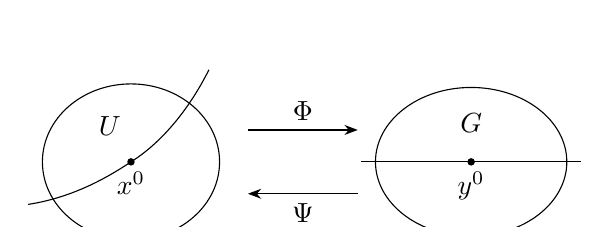
\begin{tikzpicture}[scale=.9]
\draw(0,0)ellipse(1.25 and 1.1);
\draw(-1.45,-.6)..controls(-.8,-.5)and(-.3,-.2)..(0,0)..controls(.4,.25)and(.8,.7)..(1.1,1.3);
\node at(-.3,.5){$U$};\fill(0,0)circle(1.5pt);\node[below]at(0,0){$x^0$};
\draw[-{Stealth}](1.65,.45)--(3.2,.45)node[midway,above]{$\Phi$};
\draw[-{Stealth}](3.2,-.45)--(1.65,-.45)node[midway,below]{$\Psi$};
\draw(4.8,0)ellipse(1.35 and 1.05);\draw(3.25,0)--(6.35,0);
\node at(4.8,.55){$G$};\fill(4.8,0)circle(1.5pt);\node[below]at(4.8,0){$y^0$};
\end{tikzpicture}
\end{center}
\ednote{该范数比较须在坐标变换及其逆具有足够正则性和一致界的局部区域上使用。
对 $W^{k,p}$，可要求二者的至 $k$ 阶导数有界，且 Jacobian 不退化。
仅有 $C^1$ 边界时，不能直接将其展平变换用于任意高阶 $W^{k,p}$；下面的逼近证明在原坐标的局部图像上作平移。}

\subsection*{3. 直到边界的整体逼近（续）}
\source{9.21/02、03}
\proofrating{01}{4}{精读：边界平移、磨光和单位分解组成常用逼近方法。}
\textbf{定理。}设 $U\subset\R^n$ 为有界开集，$\partial U$ 是 $C^1$ 的，
$1\leq p<\infty$，$u\in W^{k,p}(U)$。则存在
\[
\{u_m\}_{m=1}^{\infty}\subset C^\infty(\overline U),\qquad
u_m\longrightarrow u\quad\text{于 }W^{k,p}(U).
\]

\newpage
\subsection*{证明：$1^\circ$ 边界附近的平移与磨光}
\source{9.21/02--04；06 中重复的估计合并}
\proofrating{01（续）}{4}{重点：先平移避开边界，再磨光；理解顺序及误差控制。}
给定 $x^0\in\partial U$，令
\[
V=U\cap B\left(x^0,\frac r2\right).
\]
定义
\[
u_j(x)=u\left(x+\frac1j e_n\right),\quad x\in U_j,\qquad
U_j=\left\{x:x+\frac1j e_n\in U\right\}.
\]
则 $u_j\in W^{k,p}(U_j)$，且当 $j$ 充分大时，$V\Subset U_j$。
\ednote{取边界点附近的坐标，使 $U$ 在 $C^1$ 图像 $x_n=\gamma(x')$ 上方；
$e_n$ 指向区域内部，$r$ 取在该局部图像的范围内。这里的 $V\Subset U_j$ 指
$\overline V$ 包含在平移后区域 $U_j$ 的内部。}
\begin{center}
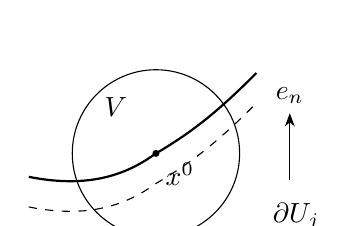
\begin{tikzpicture}[scale=.85]
\draw(0,0)circle(1.25);
\draw[thick](-1.9,-.35)..controls(-.9,-.55)and(-.35,-.25)..(0,0)..controls(.6,.35)and(1,.7)..(1.5,1.2);
\draw[dashed](-1.9,-.8)..controls(-.9,-1)and(-.35,-.7)..(0,-.45)..controls(.6,-.1)and(1,.25)..(1.5,.75);
\fill(0,0)circle(1.5pt);\node[below right]at(0,0){$x^0$};
\node at(-.6,.7){$V$};\draw[-{Stealth}](2,-.4)--(2,.6)node[above]{$e_n$};
\node[right]at(1.6,-.95){$\partial U_j$};
\end{tikzpicture}
\end{center}
由 $L^p$ 中平移的连续性，任给 $\sigma>0$，存在充分大的 $j_0$，使
\[
\|D^\alpha u_{j_0}-D^\alpha u\|_{L^p(V)}<\sigma,
\qquad\forall\alpha:\ |\alpha|\leq k.
\]
令 $v^\varepsilon=\eta_\varepsilon*u_{j_0}$。当 $\varepsilon$ 充分小时，
\[
v^\varepsilon\in C^\infty(\overline V),\qquad
\|v^\varepsilon-u_{j_0}\|_{W^{k,p}(V)}\longrightarrow0.
\]
因此存在充分小的 $\varepsilon_0>0$，使对所有 $|\alpha|\leq k$，
\[
\|D^\alpha v^{\varepsilon_0}-D^\alpha u_{j_0}\|_{L^p(V)}<\sigma,
\]
从而
\[
\boxed{\|D^\alpha v^{\varepsilon_0}-D^\alpha u\|_{L^p(V)}<2\sigma.}
\]

\newpage
\subsection*{证明：$2^\circ$ 有限覆盖与单位分解}
\source{9.21/05--07}
\proofrating{01（续）}{4}{重点：用单位分解将局部逼近拼成整体逼近。}
由于 $\partial U$ 紧，存在有限个点 $x_i^0\in\partial U$ 及 $r_i>0$，使
\[
\partial U\subset\bigcup_{i=1}^N B\left(x_i^0,\frac{r_i}{2}\right).
\]
令 $V_i=U\cap B(x_i^0,r_i/2)$，再取 $V_0\Subset U$，使
\[
U=\bigcup_{i=0}^N V_i,\qquad
\overline U\subset V_0\cup\bigcup_{i=1}^N B\left(x_i^0,\frac{r_i}{2}\right).
\]
\begin{center}
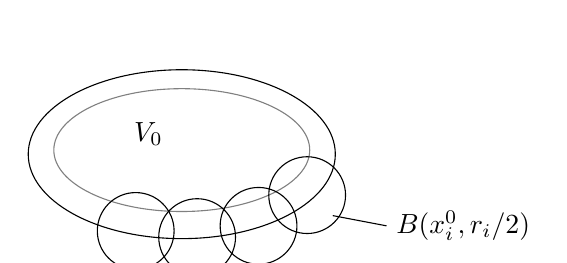
\begin{tikzpicture}[scale=.65]
\draw(0,0)ellipse(3 and 1.65);\draw[gray](0,.08)ellipse(2.5 and 1.2);
\node at(-.65,.4){$V_0$};
\foreach \x/\y in {-.9/-1.5,.3/-1.62,1.5/-1.4,2.45/-.8}{\draw(\x,\y)circle(.75);}
\draw(2.95,-1.2)--(4,-1.4)node[right]{$B(x_i^0,r_i/2)$};
\end{tikzpicture}
\end{center}
任给 $\delta>0$，由 $1^\circ$，存在 $v_i\in C^\infty(\overline V_i)$，使
\[
\|v_i-u\|_{W^{k,p}(V_i)}<\delta,\qquad i=1,\ldots,N.
\]
由内部逼近，存在 $v_0\in C^\infty(\overline V_0)$，使
$\|v_0-u\|_{W^{k,p}(V_0)}<\delta$。
取 $C^\infty$ 单位分解
\[
\zeta_0\in C_c^\infty(V_0),\qquad
\zeta_i\in C_c^\infty\left(B\left(x_i^0,\frac{r_i}{2}\right)\right),
\qquad\sum_{i=0}^N\zeta_i=1\quad\text{于 }\overline U.
\]
令 $v=\sum_{i=0}^N\zeta_i v_i$。对任意 $|\alpha|\leq k$，
\[
\begin{aligned}
\|D^\alpha v-D^\alpha u\|_{L^p(U)}
&\leq\sum_{i=0}^N\|D^\alpha[\zeta_i(v_i-u)]\|_{L^p(V_i)}\\
&\leq C\sum_{i=0}^N\|v_i-u\|_{W^{k,p}(V_i)}
<C(N+1)\delta.
\end{aligned}
\]
\ednote{$v\in C^\infty(\overline U)$，且 $\delta$ 可任意小，故得到定理中的逼近列。
照片 06--07 的求导记号较简略，这里用括号明确 $D^\alpha$ 作用于整个乘积。}

\newpage
\section{延拓}
\source{9.21/07}
\proofrating{02}{4}{精读：反射、弱导数识别、展平和拼接的整体构造。}
\textbf{定理。}设 $U\subset\R^n$ 为有界开集，$\partial U$ 是 $C^1$ 的，
$1\leq p\leq\infty$。又设 $V\subset\R^n$ 为有界开集且 $U\Subset V$。
则存在有界线性算子
\[
E:W^{1,p}(U)\longrightarrow W^{1,p}(\R^n),
\]
使得
\[
\begin{aligned}
\text{(i)}\quad &Eu=u\quad\text{a.e. 于 }U,
&&\forall u\in W^{1,p}(U),\\
\text{(ii)}\quad &\operatorname{supp}Eu\subset V,\\
\text{(iii)}\quad &\|Eu\|_{W^{1,p}(\R^n)}\leq C\|u\|_{W^{1,p}(U)}.
\end{aligned}
\]
\subsection*{证明：$1^\circ$ 平边界附近的反射延拓}
\source{9.21/08--10；重复定义合并}
\proofrating{02（续）}{4}{重点：反射构造；弱导数与边界项的验证接下一页。}
先在边界点 $x^0$ 的邻域 $W$ 内构造 $\overline u$，使
\[
\|\overline u\|_{W^{1,p}(W)}\leq C\|u\|_{W^{1,p}(U)}.
\]
设 $x^0$ 附近的边界是平的。取以 $x^0$ 为中心的小球 $B$，令
\[
B^+=\{x\in B:x_n>0\}\subset U,\qquad
B^-=\{x\in B:x_n<0\}\subset\R^n\setminus\overline U.
\]
记 $x'=(x_1,\ldots,x_{n-1})$，定义
\[
\overline u(x)=\begin{cases}
u(x',x_n),&x\in B^+,\\
u(x',-x_n),&x\in B^-.
\end{cases}
\]
\begin{center}
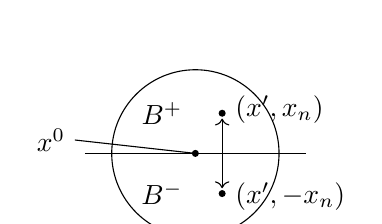
\begin{tikzpicture}[scale=.85]
\draw(0,0)circle(1.25);\draw(-1.65,0)--(1.65,0);
\node at(-.5,.6){$B^+$};\node at(-.5,-.6){$B^-$};
\fill(.4,.6)circle(1.5pt);\fill(.4,-.6)circle(1.5pt);
\draw[<->](.4,.52)--(.4,-.52);\node[right]at(.45,.65){$(x',x_n)$};
\node[right]at(.45,-.65){$(x',-x_n)$};\fill(0,0)circle(1.5pt);
\draw(0,0)--(-1.8,.2)node[left]{$x^0$};
\end{tikzpicture}
\end{center}
\ednote{经平移令 $x_n^0=0$。分界面 $x_n=0$ 是零测集，其上的取值不影响 Sobolev 类。}

\newpage
\subsection*{反射延拓的弱导数}
\source{9.21/10--12、14；分部积分重复内容仅录一次}
\proofrating{02（续）}{4}{重点：分部积分后边界项相消，保证没有额外边界项。}
因为 $u\in W^{1,1}(U)$，存在 $u_m\in C^\infty(\overline U)$，使
\[
u_m\longrightarrow u\quad\text{于 }W^{1,1}(U).
\]
\ednote{$U$ 有界，故 $u\in W^{1,p}(U)$ 蕴含 $u\in W^{1,1}(U)$，包括 $p=\infty$。
这里仅用 $W^{1,1}$ 逼近来识别弱导数，不要求在 $W^{1,\infty}$ 中光滑逼近。}
对任意 $\phi\in C_c^\infty(B)$，作反射换元，得到
\[
\begin{aligned}
-\int_B\overline u\phi_{x_n}\dd x
={}&\lim_{m\to\infty}\Bigg[
-\int_{B^+}u_m(x',x_n)\phi_{x_n}(x',x_n)\dd x\\
&\hspace{24mm}+\int_{B^+}u_m(y',y_n)
\frac{\partial\phi(y',-y_n)}{\partial y_n}\dd y\Bigg].
\end{aligned}
\]
记 $\Gamma=B\cap\{x_n=0\}$。分部积分后，上式等于
\[
\begin{aligned}
\lim_{m\to\infty}\Bigg[{}
&\int_\Gamma u_m(x',0)\phi(x',0)\dd x'
+\int_{B^+}(u_m)_{x_n}(x',x_n)\phi(x',x_n)\dd x\\
&-\int_\Gamma u_m(y',0)\phi(y',0)\dd y'
-\int_{B^+}(u_m)_{y_n}(y',y_n)\phi(y',-y_n)\dd y\Bigg].
\end{aligned}
\]
两个边界积分相消。因此
\[
-\int_B\overline u\phi_{x_n}\dd x
=\int_{B^+}u_{x_n}(x',x_n)\phi(x',x_n)\dd x
+\int_{B^-}\frac{\partial u(x',-x_n)}{\partial x_n}\phi(x',x_n)\dd x.
\]
故 $\overline u_{x_n}$ 存在，且
\[
\overline u_{x_n}(x)=\begin{cases}
u_{x_n}(x',x_n),&x\in B^+,\\
\displaystyle\frac{\partial u(x',-x_n)}{\partial x_n}
=-u_{x_n}(x',-x_n),&x\in B^-.
\end{cases}
\]
\[
\|\overline u_{x_n}\|_{L^p(B)}\leq C\|u_{x_n}\|_{L^p(B^+)},
\qquad
\boxed{\|\overline u\|_{W^{1,p}(B)}\leq C\|u\|_{W^{1,p}(B^+)}.}
\]
\ednote{保留板书对复合函数的求导记号，并写明反射产生的负号。切向导数同理，
在 $B^-$ 上为 $u_{x_i}(x',-x_n)$（$i<n$），由此得到完整范数估计。}

\newpage
\subsection*{证明：$2^\circ$ 一般边界的局部延拓}
\source{9.21/13--15；16、17 的重复示意图合并}
\proofrating{02（续）}{4}{掌握展平、反射、再变回原坐标的三步。}
利用边界展平变换 $y=\Phi(x)$、$x=\Psi(y)$。在展平后的区域内取小球 $B$，令
\[
W=\Psi(B),\qquad W^+=\Psi(B^+),\qquad u^*(y)=u(\Psi(y)).
\]
\begin{center}
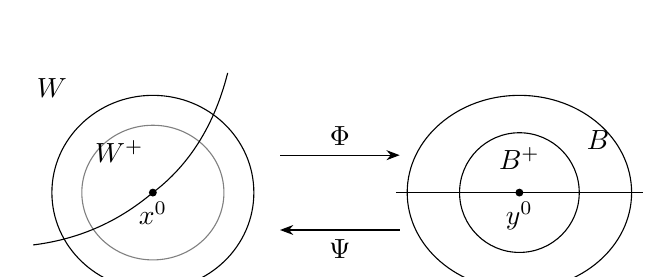
\begin{tikzpicture}[scale=.95]
\draw(0,0)ellipse(1.35 and 1.3);\draw[gray](0,0)ellipse(.95 and .9);
\draw(-1.6,-.7)..controls(-.8,-.6)and(-.3,-.25)..(0,0)..controls(.4,.3)and(.8,.8)..(1,1.6);
\node at(-.45,.55){$W^+$};\node at(-1.35,1.4){$W$};
\fill(0,0)circle(1.5pt);\node[below]at(0,0){$x^0$};
\draw[-{Stealth}](1.7,.5)--(3.3,.5)node[midway,above]{$\Phi$};
\draw[-{Stealth}](3.3,-.5)--(1.7,-.5)node[midway,below]{$\Psi$};
\draw(4.9,0)ellipse(1.5 and 1.3);\draw(4.9,0)circle(.8);
\draw(3.25,0)--(6.55,0);\node at(4.9,.45){$B^+$};
\node at(5.95,.7){$B$};\fill(4.9,0)circle(1.5pt);\node[below]at(4.9,0){$y^0$};
\end{tikzpicture}
\end{center}
对 $u^*$ 作上述反射延拓，记作 $\overline{u^*}$，则
\[
\|\overline{u^*}\|_{W^{1,p}(B)}\leq C\|u^*\|_{W^{1,p}(B^+)}.
\]
再令
\[
\overline u(x)=\overline{u^*}(\Phi(x)),\qquad x\in W.
\]
利用坐标变换的范数比较，
\[
\begin{aligned}
\|\overline u\|_{W^{1,p}(W)}
&\leq C\|\overline{u^*}\|_{W^{1,p}(B)}\\
&\leq C\|u^*\|_{W^{1,p}(B^+)}\\
&\leq C\|u\|_{W^{1,p}(U)}.
\end{aligned}
\]
\ednote{这里仅涉及一阶 Sobolev 空间；在适当缩小的坐标邻域内，$C^1$ 展平变换及其逆的导数有界，可使用上述估计。}

\newpage
\subsection*{证明：有限覆盖拼接为全空间延拓}
\source{9.21/15--17}
\proofrating{02（续）}{4}{掌握局部到整体的拼接，具体求和估计可快速核对。}
由于 $\partial U$ 紧，存在有限个点 $x_i^0\in\partial U$、包含它们的开集 $W_i$，
以及到 $W_i$ 的局部延拓 $\overline u_i$，使得
\[
\partial U\subset\bigcup_{i=1}^N W_i,\qquad
\|\overline u_i\|_{W^{1,p}(W_i)}\leq C\|u\|_{W^{1,p}(U)}.
\]
取 $W_0\Subset U$，使
\[
\overline U\subset\bigcup_{i=0}^N W_i.
\]
\ednote{照片 15--17 开头写成“$\partial W$ 紧”，由紧接着的覆盖式可知此处应为
“$\partial U$ 紧”，已改正。各 $W_i$ 可取在给定的 $V$ 内。}
取相应的光滑单位分解 $\{\zeta_i\}_{i=0}^N$，令
\[
\overline u(x)=\sum_{i=0}^N\zeta_i(x)\overline u_i(x),\qquad
\overline u_0=u.
\]
则 $\overline u\in W^{1,p}(\R^n)$。验证：
\[
\text{(i)}\qquad
\sum_{i=0}^N\zeta_i\overline u_i
=\sum_{i=0}^N\zeta_i u=u\quad\text{于 }U;
\]
\[
\text{(ii)}\qquad\operatorname{supp}\overline u\subset V;
\]
\[
\text{(iii)}\qquad\|\overline u\|_{W^{1,p}(\R^n)}\leq C\|u\|_{W^{1,p}(U)}.
\]
\ednote{每项 $\zeta_i\overline u_i$ 在 $W_i$ 外延拓为零。取
$\zeta_i\in C_c^\infty(W_i)$，且 $\sum_i\zeta_i=1$ 于 $\overline U$，便保证拼接及支撑条件。
板书将 (iii) 标为勾号；该估计由乘积公式、局部范数估计及有限求和得到。
固定这些坐标与单位分解后，令 $Eu=\overline u$，构造对 $u$ 是线性的。}

\clearpage
\fancyhead[R]{\small 2026 年 9 月 23 日}
\begin{center}
{\LARGE\bfseries 9 月 23 日课堂板书}\\[4pt]
{延拓补充、迹与零边界值}
\end{center}
\subsection*{接上次课：二阶延拓的注记}
\source{9.23/01 左侧}
\proofrating{03}{2}{可略读：二阶反射系数与导数配对的补充推导。}
设 $U\subset\R^n$ 为有界开集，$\partial U$ 是 $C^2$ 的，$u\in W^{2,p}(U)$。
在平边界的局部坐标中，令
\[
\overline u(x)=\begin{cases}
u(x',x_n),&x\in B^+,\\
-3u(x',-x_n)+4u\left(x',-\dfrac{x_n}{2}\right),&x\in B^-.
\end{cases}
\]
在 $B^-$ 上，法向导数为
\[
\overline u_{x_n}(x)
=3u_{x_n}(x',-x_n)-2u_{x_n}\left(x',-\frac{x_n}{2}\right).
\]
\ednote{沿用上次课 $B^\pm$、$x'$ 的记号。系数满足 $-3+4=1$、$3-2=1$，
使函数及一阶法向导数在分界面两侧相匹配；这里保留板书给出的二阶延拓公式。}

\section{迹}
\source{9.23/01 右侧、02 左侧}
\proofrating{04}{5}{优先掌握：边界估计、稠密逼近与迹算子的定义。}
\textbf{定理。}设 $U\subset\R^n$ 为有界开集，$\partial U$ 是 $C^1$ 的，
$1\leq p<\infty$。则存在有界线性算子
\[
T:W^{1,p}(U)\longrightarrow L^p(\partial U),\qquad u\longmapsto Tu,
\]
使得
\[
\text{(i)}\quad Tu=u|_{\partial U},\qquad
\forall u\in W^{1,p}(U)\cap C(\overline U),
\]
\[
\text{(ii)}\quad\|Tu\|_{L^p(\partial U)}\leq C\|u\|_{W^{1,p}(U)},
\qquad C=C(p,U).
\]
\textbf{证明。}先定义
\[
T:C^1(\overline U)\longrightarrow L^p(\partial U),\qquad
u\longmapsto u|_{\partial U}.
\]
设 $u\in C^1(\overline U)$，给定 $x^0\in\partial U$，先证局部估计
\[
\int_\Gamma|u|^p\dd S\leq C\int_U\bigl(|u|^p+|Du|^p\bigr)\dd x.
\]

\newpage
\subsection*{迹定理的证明：局部估计}
\source{9.23/02 右侧、03}
\proofrating{04（续）}{5}{核心：把边界积分变成内部积分，再用范数控制。}
\textbf{$1^\circ$ 平边界。}取同心球 $\widehat B\Subset B$，令
$\Gamma=\widehat B\cap\{x_n=0\}$。取
\[
\zeta\in C_c^\infty(B),\qquad 0\leq\zeta\leq1,\qquad
\zeta=1\quad\text{于 }\widehat B.
\]
\begin{center}
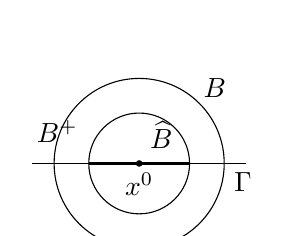
\begin{tikzpicture}[scale=.8]
\draw(0,0)circle(1.35);\draw(0,0)circle(.8);
\draw(-1.7,0)--(1.7,0);\draw[very thick](-.8,0)--(.8,0);
\fill(0,0)circle(1.5pt);\node[below]at(0,0){$x^0$};
\node at(.35,.45){$\widehat B$};\node at(1.2,1.2){$B$};
\node at(-1.3,.5){$B^+$};\node at(1.65,-.3){$\Gamma$};
\end{tikzpicture}
\end{center}
\[
\begin{aligned}
\int_\Gamma|u|^p\dd x'
&\leq\int_{\{x_n=0\}}\zeta|u|^p\dd x'\\
&=-\int_{B^+}(\zeta|u|^p)_{x_n}\dd x\\
&=-\int_{B^+}\left(\zeta_{x_n}|u|^p
+\zeta p|u|^{p-2}u u_{x_n}\right)\dd x\\
&\leq C\int_{B^+}\bigl(|u|^p+|Du|^p\bigr)\dd x.
\end{aligned}
\]
\ednote{最后一步估计 $|u|^{p-1}|u_{x_n}|$。上面的经典链式公式按 $p>1$ 写出；
当 $p=1$ 时使用 $|\partial_{x_n}|u||\leq|u_{x_n}|$ 的几乎处处形式，得到相同估计。}
\textbf{$2^\circ$ 一般边界。}用 $\Phi$ 将边界展平，$\Psi=\Phi^{-1}$。
\begin{center}
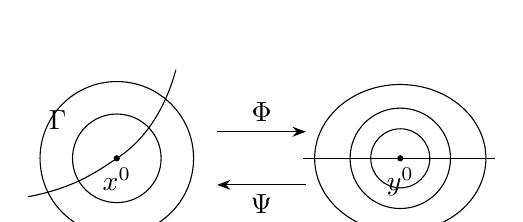
\begin{tikzpicture}[scale=.75]
\draw(0,0)circle(1.3);\draw(0,0)circle(.75);
\draw(-1.5,-.65)..controls(-.7,-.5)and(-.3,-.2)..(0,0)..controls(.4,.25)and(.8,.75)..(1,1.5);
\node at(-1,.65){$\Gamma$};\fill(0,0)circle(1.5pt);\node[below]at(0,0){$x^0$};
\draw[-{Stealth}](1.7,.45)--(3.2,.45)node[midway,above]{$\Phi$};
\draw[-{Stealth}](3.2,-.45)--(1.7,-.45)node[midway,below]{$\Psi$};
\draw(4.8,0)ellipse(1.45 and 1.25);\draw(4.8,0)circle(.85);\draw(4.8,0)circle(.5);
\draw(3.15,0)--(6.4,0);\fill(4.8,0)circle(1.5pt);\node[below]at(4.8,0){$y^0$};
\end{tikzpicture}
\end{center}
于是仍有
\[
\int_\Gamma|u|^p\dd S\leq C\int_U\bigl(|u|^p+|Du|^p\bigr)\dd x.
\]

\newpage
\subsection*{迹定理的证明：全局构造与连续函数的边界值}
\source{9.23/04--06；重复的极限推导合并}
\proofrating{04（续）}{5}{核心：用估计保证边界值极限存在且与逼近列无关。}
由于 $\partial U$ 紧，可取有限个 $x_i^0\in\partial U$ 及相应的 $\Gamma_i$，使
\[
\partial U\subset\bigcup_{i=1}^N\Gamma_i,\qquad
\|u\|_{L^p(\Gamma_i)}\leq C\|u\|_{W^{1,p}(U)}.
\]
因而对 $u\in C^1(\overline U)$，$\|Tu\|_{L^p(\partial U)}\leq C\|u\|_{W^{1,p}(U)}$。
任给 $u\in W^{1,p}(U)$，取 $\{u_m\}\subset C^\infty(\overline U)$，使
\[
u_m\longrightarrow u\quad\text{于 }W^{1,p}(U).
\]
由
\[
\|Tu_m\|_{L^p(\partial U)}\leq C\|u_m\|_{W^{1,p}(U)},
\]
\[
\|Tu_m-Tu_l\|_{L^p(\partial U)}\leq C\|u_m-u_l\|_{W^{1,p}(U)},
\]
可知存在 $u^*\in L^p(\partial U)$，定义
\[
Tu_m\longrightarrow u^*\eqqcolon Tu\quad\text{于 }L^p(\partial U).
\]
\ednote{对两组逼近列应用同一估计可知极限与逼近列无关；取极限即得线性和有界性。}
当 $u\in W^{1,p}(U)\cap C(\overline U)$ 时，利用直到边界的整体逼近构造，
可取 $u_m\in C^\infty(\overline U)$ 同时满足
\[
u_m\to u\quad\text{于 }W^{1,p}(U),\qquad
u_m\to u\quad\text{一致于 }\overline U.
\]
因此
\[
Tu_m=u_m|_{\partial U}\longrightarrow u|_{\partial U}=Tu
\quad\text{于 }L^p(\partial U).
\]
\subsection*{注：Sobolev 函数的积分公式}
\source{9.23/06 右侧}
\proofrating{05}{2}{证明可略读：光滑逼近与迹的连续性；积分公式仍须会用。}
设 $u\in W^{1,p}(U)$，则
\[
\begin{aligned}
\int_Uu_{x_i}\dd x
&=\lim_{m\to\infty}\int_U(u_m)_{x_i}\dd x\\
&=\lim_{m\to\infty}\int_{\partial U}u_m\cos(\vec n,x_i)\dd S\\
&=\int_{\partial U}Tu\cos(\vec n,x_i)\dd S.
\end{aligned}
\]
\ednote{沿用板书的方向余弦记号：$\vec n$ 为单位外法向量，$\cos(\vec n,x_i)=n_i$。}

\newpage
\subsection{\texorpdfstring{零延拓与 $W_0^{1,p}(U)$}{零延拓与零边界值空间}}
\source{9.23/07、08}
\proofrating{06}{4}{精读：零延拓的弱导数，以及逆向的支撑内移方法。}
\textbf{定理。}设 $U\subset\R^n$ 为有界开集，$\partial U$ 是 $C^1$ 的，
$1\leq p<\infty$。对 $u:U\to\R$，令
\[
\widetilde u(x)=\begin{cases}u(x),&x\in U,\\0,&x\notin U.\end{cases}
\]
则
\[
\boxed{u\in W_0^{1,p}(U)\quad\Longleftrightarrow\quad
\widetilde u\in W^{1,p}(\R^n).}
\]
\textbf{证明。}$\Longrightarrow$：取 $u_m\in C_c^\infty(U)$，使
$u_m\to u$ 于 $W^{1,p}(U)$。对任意 $\phi\in C_c^\infty(\R^n)$，
\[
\begin{aligned}
-\int_{\R^n}\widetilde u\phi_{x_i}\dd x
&=-\int_Uu\phi_{x_i}\dd x
=-\lim_{m\to\infty}\int_Uu_m\phi_{x_i}\dd x\\
&=-\lim_{m\to\infty}\int_{\partial U}u_m\phi\cos(\vec n,x_i)\dd S
+\lim_{m\to\infty}\int_U(u_m)_{x_i}\phi\dd x\\
&=\int_Uu_{x_i}\phi\dd x=\int_{\R^n}v\phi\dd x,
\end{aligned}
\]
其中
\[
v(x)=\begin{cases}u_{x_i}(x),&x\in U,\\0,&x\notin U.\end{cases}
\]
\textbf{$\Longleftarrow$：}由于 $\partial U$ 紧，存在 $x_i^0\in\partial U$ 及 $r_i>0$，使
\[
\partial U\subset\bigcup_{i=1}^N B\left(x_i^0,\frac{r_i}{2}\right).
\]
取 $V_0\Subset U$，使 $\overline U\subset V_0\cup\bigcup_{i=1}^N B(x_i^0,r_i/2)$。
取相应的光滑单位分解
\[
\zeta_0\in C_c^\infty(V_0),\qquad
\zeta_i\in C_c^\infty\left(B\left(x_i^0,\frac{r_i}{2}\right)\right),\qquad
\sum_{i=0}^N\zeta_i=1\quad\text{于 }\overline U.
\]
于是
\[
u=\sum_{i=0}^N u\zeta_i=\sum_{i=0}^N\widetilde u\zeta_i\quad\text{于 }U,
\]
且 $\zeta_i\widetilde u\in W^{1,p}(\R^n)$；当 $i\geq1$ 时，
\[
\operatorname{supp}(\zeta_i\widetilde u)
\subset\overline U\cap B\left(x_i^0,\frac{r_i}{2}\right).
\]

\newpage
\subsection*{零延拓定理的证明（续）：将支撑移入区域内部}
\source{9.23/09 左侧}
\proofrating{06（续）}{4}{重点：支撑内移后磨光，再用平移连续性取极限。}
给定 $i\geq1$，不妨设局部区域为
\[
U\cap B\left(x_i^0,\frac{r_i}{2}\right)
=\left\{x\in B\left(x_i^0,\frac{r_i}{2}\right):
x_n>\gamma(x_1,\ldots,x_{n-1})\right\}.
\]
令 $e_n=(0,\ldots,0,1)$，定义
\[
(\zeta_i\widetilde u)^j(x)
=(\zeta_i\widetilde u)\left(x-\frac1j e_n\right),\qquad x\in\R^n.
\]
则 $(\zeta_i\widetilde u)^j\in W^{1,p}(\R^n)$，且当 $j$ 充分大时，
\[
\operatorname{supp}(\zeta_i\widetilde u)^j\Subset U.
\]
\begin{center}
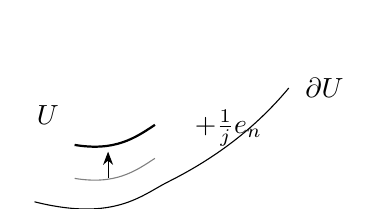
\begin{tikzpicture}[scale=.85]
\draw(-2,-.3)..controls(-.8,-.6)and(-.4,-.2)..(0,0)..controls(.7,.35)and(1.3,.8)..(1.8,1.4);
\draw[gray](-1.4,.05)..controls(-.8,-.05)and(-.5,.15)..(-.2,.35);
\draw[thick](-1.4,.55)..controls(-.8,.45)and(-.5,.65)..(-.2,.85);
\draw[-{Stealth}](-.9,.05)--(-.9,.45);
\node at(-1.8,1){$U$};\node[right]at(.25,.8){$+\frac1j e_n$};
\node[right]at(1.9,1.4){$\partial U$};
\end{tikzpicture}
\end{center}
因此
\[
(\zeta_i\widetilde u)^j\in W_0^{1,p}(U)
\quad\Longrightarrow\quad\zeta_i\widetilde u\in W_0^{1,p}(U).
\]
\ednote{支撑在 $U$ 内紧包含的 Sobolev 函数可经磨光由 $C_c^\infty(U)$ 逼近；
平移在 $W^{1,p}(\R^n)$ 中连续。令 $j\to\infty$ 并用 $W_0^{1,p}(U)$ 的闭性即得结论。
$i=0$ 的一项本来就紧支撑于 $U$，最后有限求和得到 $u\in W_0^{1,p}(U)$。}

\subsection{零迹与零边界值空间}
\source{9.23/09 右侧；证明接 9 月 28 日}
\proofrating{07}{4}{精读：零迹与零边界值空间的联系；证明接下一次课。}
\textbf{定理。}设 $U\subset\R^n$ 为有界开集，$\partial U$ 是 $C^1$ 的，
$1\leq p<\infty$，$u\in W^{1,p}(U)$。则
\[
\boxed{u\in W_0^{1,p}(U)\quad\Longleftrightarrow\quad Tu=0\quad\text{于 }\partial U.}
\]
\ednote{边界上的等式按 $L^p(\partial U)$ 的几乎处处意义理解。}
\clearpage
\fancyhead[R]{\small 2026 年 9 月 28 日}
\begin{center}
{\LARGE\bfseries 9 月 28 日课堂板书}\\[4pt]
{零迹定理续证与 Sobolev 不等式}
\end{center}
\subsection*{零迹定理的证明（接 9 月 23 日）}
\source{9.28/01--03；重复的定理陈述不再抄写}
\proofrating{07（续）}{4}{重点：零迹使边界积分消失，再识别零延拓的弱导数。}
\textbf{$\Longrightarrow$：}板书标为已证。
\ednote{取 $u_m\in C_c^\infty(U)$ 在 $W^{1,p}(U)$ 中逼近 $u$，由迹算子的连续性及 $Tu_m=0$ 得 $Tu=0$。}
\textbf{$\Longleftarrow$：}设 $Tu=0$。令 $\widetilde u$ 为 $u$ 的零延拓，下证
$\widetilde u\in W^{1,p}(\R^n)$。
由整体逼近，存在 $\{u_m\}_{m=1}^\infty\subset C^\infty(\overline U)$，使
\[
u_m\to u\quad\text{于 }W^{1,p}(U),\qquad
Tu_m=u_m|_{\partial U}\to0\quad\text{于 }L^p(\partial U).
\]
对任意 $\phi\in C_c^\infty(\R^n)$，
\[
\begin{aligned}
-\int_{\R^n}\widetilde u\phi_{x_i}\dd x
&=-\int_Uu\phi_{x_i}\dd x
=-\lim_{m\to\infty}\int_Uu_m\phi_{x_i}\dd x\\
&=-\lim_{m\to\infty}\int_{\partial U}u_m\phi\cos(\vec n,x_i)\dd S
+\lim_{m\to\infty}\int_U(u_m)_{x_i}\phi\dd x\\
&=\int_Uu_{x_i}\phi\dd x=\int_{\R^n}v\phi\dd x,
\end{aligned}
\]
其中
\[
v(x)=\begin{cases}u_{x_i}(x),&x\in U,\\0,&x\notin U.\end{cases}
\]
所以 $\widetilde u\in W^{1,p}(\R^n)$，由零延拓定理得 $u\in W_0^{1,p}(U)$。

\section{Sobolev 不等式}
\source{9.28/03 右侧}
\textbf{定义。}设 $X,Y$ 为赋范线性空间。称 $X$ 可嵌入 $Y$，若：
\[
\text{(i)}\quad X\text{ 是 }Y\text{ 的线性子空间};\qquad
\text{(ii)}\quad I:X\to Y\text{ 是有界线性算子}.
\]
\ednote{$I$ 是包含映射 $Iu=u$；条件 (ii) 即 $\|u\|_Y\leq C\|u\|_X$。}
对于 $W^{1,p}(U)$，板书将参数分为
\[
1\leq p<n,\qquad p=n,\qquad n<p<\infty,\qquad p=\infty.
\]

\newpage
\subsection{Gagliardo--Nirenberg--Sobolev 不等式}
\source{9.28/04、05}
\proofrating{08}{4}{精读缩放论证：用尺度幂次确定临界可积指数。}
设 $1\leq p<n$。是否存在 $1\leq q\leq\infty$、$C>0$，使
\[
\|u\|_{L^q(\R^n)}\leq C\|Du\|_{L^p(\R^n)},
\qquad\forall u\in C_c^\infty(\R^n)?
\]
假设上式成立，固定非零 $u\in C_c^\infty(\R^n)$。
对任意 $\lambda>0$，令
\[
u_\lambda(x)=u(\lambda x),\qquad x\in\R^n.
\]
则 $\|u_\lambda\|_{L^q(\R^n)}\leq C\|Du_\lambda\|_{L^p(\R^n)}$。
作换元 $y=\lambda x$，
\[
\begin{aligned}
\|u_\lambda\|_{L^q(\R^n)}
&=\left(\int_{\R^n}|u(\lambda x)|^q\dd x\right)^{1/q}\\
&=\lambda^{-n/q}\left(\int_{\R^n}|u(y)|^q\dd y\right)^{1/q},
\end{aligned}
\]
\[
\begin{aligned}
\|Du_\lambda\|_{L^p(\R^n)}
&=\left(\int_{\R^n}|\lambda Du(\lambda x)|^p\dd x\right)^{1/p}\\
&=\lambda^{1-n/p}\left(\int_{\R^n}|Du(y)|^p\dd y\right)^{1/p}.
\end{aligned}
\]
因此，对所有 $\lambda>0$，
\[
\left(\int_{\R^n}|u|^q\right)^{1/q}
\leq C\lambda^{1-n/p+n/q}\left(\int_{\R^n}|Du|^p\right)^{1/p}.
\]
必有
\[
1-\frac np+\frac nq=0,\qquad\text{即}\qquad q=\frac{np}{n-p}.
\]
\ednote{若指数不为零，分别令 $\lambda\to0$ 或 $\lambda\to\infty$ 会与 $u\ne0$ 矛盾。
当 $q=\infty$ 时用 $\|u_\lambda\|_\infty=\|u\|_\infty$，并约定 $1/q=0$。}
\textbf{定义。}称
\[
p^*\coloneqq\frac{np}{n-p}
\]
为 $p$ 的 Sobolev 共轭指数，且 $p^*>p$。
\proofrating{09}{5}{GNS 核心证明从下一页开始；优先掌握两个参数情形的衔接。}
\textbf{定理。}设 $1\leq p<n$，则存在 $C=C(n,p)$，使
\[
\boxed{\|u\|_{L^{p^*}(\R^n)}\leq C\|Du\|_{L^p(\R^n)},
\qquad\forall u\in C_c^1(\R^n).}
\]

\newpage
\subsection*{证明：$1^\circ$ $p=1$ 的情形}
\source{9.28/06--07}
\proofrating{09}{5}{GNS 核心证明：从一维积分出发，用多因子 Hölder 估计。}
\textbf{板书旁记：多因子 Hölder 不等式。}
设 $1\leq p_i\leq\infty$，$i=1,\ldots,k$，且
$\sum_{i=1}^k1/p_i=1$。若 $f_i\in L^{p_i}(E)$，则
\[
f_1\cdots f_k\in L^1(E),\qquad
\|f_1\cdots f_k\|_{L^1(E)}
\leq\|f_1\|_{L^{p_1}(E)}\cdots\|f_k\|_{L^{p_k}(E)}.
\]
现在证明
\[
\|u\|_{L^{n/(n-1)}(\R^n)}\leq C\|Du\|_{L^1(\R^n)}.
\]
对每个 $i=1,\ldots,n$，
\[
u(x)=\int_{-\infty}^{x_i}
u_{x_i}(x_1,\ldots,y_i,\ldots,x_n)\dd y_i,
\]
因而
\[
|u(x)|\leq\int_{-\infty}^{\infty}
|Du(x_1,\ldots,y_i,\ldots,x_n)|\dd y_i.
\]
将 $n$ 个估计相乘并取 $1/(n-1)$ 次幂，得
\[
|u(x)|^{n/(n-1)}
\leq\prod_{i=1}^n
\left(\int_\R|Du(x_1,\ldots,y_i,\ldots,x_n)|\dd y_i\right)^{1/(n-1)}.
\]
先对 $x_1$ 积分：
\[
\begin{aligned}
\int_\R|u(x)|^{n/(n-1)}\dd x_1
\leq{}&
\left(\int_\R|Du(y_1,x_2,\ldots,x_n)|\dd y_1\right)^{1/(n-1)}\\
&\quad\times\int_\R\prod_{i=2}^n
\left(\int_\R|Du(x_1,\ldots,y_i,\ldots,x_n)|\dd y_i\right)^{1/(n-1)}
\dd x_1\\
\leq{}&
\left(\int_\R|Du(y_1,x_2,\ldots,x_n)|\dd y_1\right)^{1/(n-1)}\\
&\quad\times\prod_{i=2}^n
\left(\int_\R\int_\R|Du(x_1,\ldots,y_i,\ldots,x_n)|
\dd x_1\dd y_i\right)^{1/(n-1)}.
\end{aligned}
\]
\ednote{第一因子不含 $x_1$，故可提出；对其余 $n-1$ 个因子应用 Hölder 不等式。
照片 07 部分板书被遮挡，此处结合 08--10 的连续推导连接。}

\newpage
\subsection*{$p=1$ 的证明（续）：逐个变量积分}
\source{9.28/08--10 左侧}
\proofrating{09（续）}{5}{理解逐变量积分的结构，避免只背多重积分展开式。}
继续对 $x_2$ 积分，再用 Hölder 不等式，得到
\[
\begin{aligned}
\int_\R\int_\R|u(x)|^{n/(n-1)}\dd x_1\dd x_2
\leq{}&
\left(\int_\R\int_\R
|Du(x_1,y_2,x_3,\ldots,x_n)|\dd x_1\dd y_2\right)^{1/(n-1)}\\
&\times\left(\int_\R\int_\R
|Du(y_1,x_2,x_3,\ldots,x_n)|\dd y_1\dd x_2\right)^{1/(n-1)}\\
&\times\prod_{i=3}^n
\left(\int_\R\int_\R\int_\R
|Du(x_1,\ldots,y_i,\ldots,x_n)|
\dd x_1\dd x_2\dd y_i\right)^{1/(n-1)}.
\end{aligned}
\]
依次对 $x_3,\ldots,x_n$ 积分，最后得到
\[
\begin{aligned}
\int_{\R^n}|u(x)|^{n/(n-1)}\dd x
&\leq\prod_{i=1}^n
\left(\int_\R\cdots\int_\R
|Du(x_1,\ldots,y_i,\ldots,x_n)|
\dd x_1\cdots\dd y_i\cdots\dd x_n\right)^{1/(n-1)}\\
&=\left(\int_{\R^n}|Du|\dd x\right)^{n/(n-1)}.
\end{aligned}
\]
所以
\[
\boxed{\left(\int_{\R^n}|u|^{n/(n-1)}\dd x\right)^{(n-1)/n}
\leq\int_{\R^n}|Du|\dd x.}
\]
\ednote{第二轮的展开式按 $n\geq3$ 写出；$n=2$ 时，第一轮后再作一次积分即可得到结论。
后续各轮将已合并的相同因子一起使用 Hölder 不等式。以上保留板书的逐变量积分次序。}

\subsection*{证明：$2^\circ$ $1<p<n$ 的情形}
\source{9.28/10 右侧}
\proofrating{09（续）}{5}{核心技巧：对函数取幂，把一般情形归约到 $p=1$。}
令
\[
v=|u|^\gamma,\qquad\gamma>1\text{ 待定}.
\]
对 $v$ 使用 $p=1$ 的结论：
\[
\left(\int_{\R^n}|v|^{n/(n-1)}\dd x\right)^{(n-1)/n}
\leq\int_{\R^n}|Dv|\dd x.
\]

\newpage
\subsection*{$1<p<n$ 的证明（续）}
\source{9.28/10、11 左侧、12 左侧；重复内容合并}
\proofrating{09（续）}{5}{掌握幂指数的选取及公共因子的消去。}
\[
\begin{aligned}
\left(\int_{\R^n}|u|^{n\gamma/(n-1)}\dd x\right)^{(n-1)/n}
&\leq\gamma\int_{\R^n}|u|^{\gamma-1}|Du|\dd x\\
&\leq\gamma\left(\int_{\R^n}|Du|^p\dd x\right)^{1/p}
\left(\int_{\R^n}|u|^{p(\gamma-1)/(p-1)}\dd x\right)^{(p-1)/p}.
\end{aligned}
\]
令
\[
\frac{n\gamma}{n-1}=\frac{p(\gamma-1)}{p-1},
\qquad\text{则}\qquad
\gamma=\frac{(n-1)p}{n-p}>1.
\]
两边的 $u$ 的积分指数均为 $p^*$，故
\[
\boxed{\left(\int_{\R^n}|u|^{p^*}\dd x\right)^{1/p^*}
\leq\gamma\left(\int_{\R^n}|Du|^p\dd x\right)^{1/p}.}
\]
\ednote{当 $u\ne0$ 时除去公共因子，并用
$(n-1)/n-(p-1)/p=1/p^*$；$u=0$ 时结论显然。}

\subsection{零边界值函数的 Sobolev 不等式}
\source{9.28/11--12；采用最后完成的板书}
\proofrating{10}{3}{理解零延拓与稠密逼近，学会将光滑函数估计传给极限。}
\textbf{定理。}设 $U\subset\R^n$ 为开集，$1\leq p<n$，$u\in W_0^{1,p}(U)$。
则 $u\in L^{p^*}(U)$，且
\[
\|u\|_{L^{p^*}(U)}\leq C\|Du\|_{L^p(U)},\qquad C=C(n,p).
\]
\textbf{证明。}存在 $\{u_m\}_{m=1}^\infty\subset C_c^\infty(U)$，使
\[
u_m\to u\quad\text{于 }W^{1,p}(U).
\]
由全空间不等式，
\[
\|u_m\|_{L^{p^*}(U)}\leq C\|Du_m\|_{L^p(U)}.
\]
因此
\[
u_m\to u\quad\text{于 }L^{p^*}(U).
\]
\ednote{此处将 $u_m$ 在 $U$ 外延拓为零后应用全空间不等式。对差 $u_m-u_l$
应用同一估计可知其在 $L^{p^*}$ 中是 Cauchy 列；结合 $L^p$ 收敛辨认极限为 $u$。
再取极限即得所需估计。照片 11 最初记极限为 $\widetilde u$，12 已改成 $u$。}

\newpage
\subsection*{有界开集上的推论}
\source{9.28/13}
\proofrating{11}{1}{证明可跳过：有限测度上的一次 Hölder 估计；记住指数范围。}
\textbf{推论。}设 $U\subset\R^n$ 为有界开集，$1\leq p<n$，$u\in W_0^{1,p}(U)$。
则对所有 $1\leq q\leq p^*$，有 $u\in L^q(U)$，且
\[
\|u\|_{L^q(U)}\leq C\|Du\|_{L^p(U)},\qquad C=C(n,p,q,U).
\]
\textbf{证明。}已知 $u\in L^{p^*}(U)$。对 $1\leq q<p^*$，使用共轭指数
\[
\frac{p^*}{q},\qquad \frac{p^*}{p^*-q},
\]
得到
\[
\begin{aligned}
\left(\int_U|u|^q\dd x\right)^{1/q}
&\leq\left(\int_U|u|^{p^*}\dd x\right)^{1/p^*}
\left(|U|^{(p^*-q)/p^*}\right)^{1/q}\\
&=|U|^{1/q-1/p^*}\|u\|_{L^{p^*}(U)}
\leq C\|Du\|_{L^p(U)}.
\end{aligned}
\]
\ednote{$q=p^*$ 时直接使用上一定理，不使用含 $p^*-q$ 分母的指数。}

\subsection*{临界情形 $p=n$}
\source{9.28/14；13 与 14 的板书修改按最终版本分别保留}
\proofrating{12}{3}{理解取略小于临界值的指数，从次临界嵌入推出有限 $q$。}
\textbf{推论。}设 $U\subset\R^n$ 为有界开集，$u\in W_0^{1,n}(U)$。
则对所有 $1\leq q<\infty$，有 $u\in L^q(U)$，且
\[
\|u\|_{L^q(U)}\leq C\|Du\|_{L^n(U)},\qquad C=C(n,q,U).
\]
\textbf{证明。}$1^\circ$ $n=1$：板书标为已知。
\[
2^\circ\quad n>1.
\]
任给 $1\leq q<\infty$，取 $1\leq p<n$ 充分靠近 $n$，使
\[
1\leq q<p^*.
\]
由于 $u\in W_0^{1,n}(U)$ 且 $p<n$，有
\[
u\in W_0^{1,p}(U)\quad\Longrightarrow\quad u\in L^q(U).
\]
\ednote{有界性给出
$\|Du\|_{L^p(U)}\leq|U|^{1/p-1/n}\|Du\|_{L^n(U)}$，
与前一推论合用即得估计。$n=1$ 时可对紧支撑光滑函数先用
$\|u\|_\infty\leq\|u'\|_1$，再由逼近推广。}

\newpage
\subsection{Poincaré 不等式}
\source{9.28/15、16 左侧}
\proofrating{13}{2}{证明可略读：由已有嵌入分情形推出；Poincaré 结论必须会用。}
\textbf{定理。}设 $U\subset\R^n$ 为有界开集，$1\leq p<\infty$。则
\[
\boxed{\|u\|_{L^p(U)}\leq C\|Du\|_{L^p(U)},\qquad
\forall u\in W_0^{1,p}(U),}
\qquad C=C(n,p,U).
\]
\textbf{证明。}$1^\circ$ $1\leq p<n$：用 $W_0^{1,p}(U)\subset L^{p^*}(U)$
及有界开集上的推论，取 $q=p$。
\[
2^\circ\quad p=n:
\]
用临界情形的推论，取 $q=n$。
\[
3^\circ\quad n<p<\infty:
\]
设 $u\in W_0^{1,p}(U)$，则 $u\in W_0^{1,n}(U)$。从而
\[
u\in L^p(U),\qquad
\|u\|_{L^p(U)}\leq C\|Du\|_{L^n(U)}
\leq C\|Du\|_{L^p(U)}.
\]
\textbf{注。}在 $W_0^{1,p}(U)$ 中，
\[
\|u\|_{W^{1,p}(U)}\quad\text{与}\quad\|Du\|_{L^p(U)}
\quad\text{等价。}
\]

\subsection{一般边界值的 Sobolev 嵌入}
\source{9.28/16}
\proofrating{14}{3}{证明接下一页：掌握“延拓到全空间，再限制回来”的方法。}
\textbf{定理。}设 $U\subset\R^n$ 为有界开集，$\partial U$ 是 $C^1$ 的，
$1\leq p<n$，$u\in W^{1,p}(U)$。则 $u\in L^{p^*}(U)$，且
\[
\|u\|_{L^{p^*}(U)}\leq C\|u\|_{W^{1,p}(U)},\qquad C=C(n,p,U).
\]
亦即 $W^{1,p}(U)$ 可嵌入到 $L^{p^*}(U)$。
\ednote{本次照片到此处的定理陈述为止，未拍到该定理的证明，故不补写。}

\newpage
\fancyhead[R]{\small 2026 年 9 月 30 日}
\begin{center}
{\LARGE\bfseries 9 月 30 日课堂板书}\\[5pt]
{Sobolev 嵌入续证、Morrey 不等式与高阶嵌入}
\end{center}

\subsection*{一般边界值的 Sobolev 嵌入：证明（接 9 月 28 日）}
\source{9.30/01--02；定理陈述已见上一页，重复部分合并}
\proofrating{14（续）}{3}{理解延拓、GNS 估计与逼近取极限的组合。}
沿用上次课的条件：$U\subset\R^n$ 为有界开集，$\partial U$ 是 $C^1$ 的，
$1\leq p<n$，$u\in W^{1,p}(U)$，$p^*=np/(n-p)$。

\textbf{证明。}由延拓定理，存在 $\overline u\in W^{1,p}(\R^n)$，使
\[
\overline u=u\quad\text{于 }U,\qquad
\operatorname{supp}\overline u\text{ 紧},
\]
并且
\[
\|\overline u\|_{W^{1,p}(\R^n)}
\leq C\|u\|_{W^{1,p}(U)}.
\]
由内部逼近，存在 $\{u_m\}_{m=1}^{\infty}\subset C_c^\infty(\R^n)$，使
\[
u_m\longrightarrow\overline u\quad\text{于 }W^{1,p}(\R^n).
\]
由 Gagliardo--Nirenberg--Sobolev 不等式，
\[
\|u_m\|_{L^{p^*}(\R^n)}
\leq C\|Du_m\|_{L^p(\R^n)}.
\]
因此
\[
u_m\longrightarrow\overline u\quad\text{于 }L^{p^*}(\R^n).
\]
最后，
\[
\begin{aligned}
\|u\|_{L^{p^*}(U)}
&\leq\|\overline u\|_{L^{p^*}(\R^n)}\\
&\leq C\|D\overline u\|_{L^p(\R^n)}
\leq C\|u\|_{W^{1,p}(U)}.
\end{aligned}
\]
\ednote{对 $u_m-u_l$ 应用同一不等式，得到 $L^{p^*}$ 中的 Cauchy 性；
结合原来的 $L^p$ 收敛辨认极限，再令 $m\to\infty$，即为板书中取极限的一步。}

\newpage
\subsection{一般边界值的临界情形}
\source{9.30/03--07 左侧；采用 04--05 擦改完成后的版本}
\proofrating{15}{2}{证明可略读：复用 12 的降指数方法；保留对端点反例的认识。}
\textbf{推论。}设 $U\subset\R^n$ 为有界开集，$\partial U$ 是 $C^1$ 的，
$u\in W^{1,n}(U)$。则对所有 $1\leq q<\infty$，有 $u\in L^q(U)$，且
\[
\|u\|_{L^q(U)}
\leq C\|u\|_{W^{1,n}(U)},\qquad C=C(n,q,U).
\]

\textbf{证明。}$1^\circ$ $n=1$。板书在区间 $[a,b]$ 上写出：
\[
|f(x)-f(y)|
=\left|\int_x^y f'(t)\dd t\right|
\leq\int_a^b|f'(t)|\dd t,
\]
从而
\[
|f(x)|\leq |f(y)|+\int_a^b|f'(t)|\dd t.
\]
\ednote{对 $y\in(a,b)$ 取平均，即得
$\|f\|_\infty\leq (b-a)^{-1}\|f\|_{L^1(a,b)}+\|f'\|_{L^1(a,b)}$。
对 $W^{1,1}$ 函数取其绝对连续代表，可使用同一计算。}

$2^\circ$ $n>1$。任给 $1\leq q<\infty$，取 $1\leq p<n$ 充分靠近 $n$，使
\[
1\leq q<p^*.
\]
于是
\[
u\in W^{1,n}(U)\subset W^{1,p}(U)\subset L^q(U).
\]
\ednote{这里用到有界区域上的 Hölder 不等式及上一页的嵌入，
相应范数估计给出推论中的常数 $C(n,q,U)$。}

\textbf{注。}当 $n>1$ 时，$q=\infty$ 的结论不成立。板书给出的例子为
\[
u(x)=\log\log\left(1+\frac1{|x|}\right),
\qquad x\in U=B(0,1).
\]
\ednote{该公式在 $x\ne0$ 处使用；原点的函数值可任意指定，不影响 Sobolev 等价类。
此例中 $u\in W^{1,n}(U)$，但在原点附近无界。照片 03 是擦改中的中间状态，
其中残留的 $q\leq p^*$ 与 $W^{1,p}$ 已按 04--05 的最终板书改为
$q<\infty$ 与 $W^{1,n}$。}

\newpage
\subsection{Morrey 不等式}
\source{9.30/07 右侧、08--10}
\proofrating{16}{5}{优先掌握：球平均、积分核与 Hölder 连续性的联系。}
\textbf{定理。}设 $n<p\leq\infty$，则存在 $C=C(n,p)$，使
\[
\boxed{\|u\|_{C^{0,\gamma}(\R^n)}
\leq C\|u\|_{W^{1,p}(\R^n)},\qquad
\forall u\in C^1(\R^n),}
\]
其中
\[
\gamma=1-\frac np.
\]
\ednote{范数有限的情形下使用此估计；$p=\infty$ 时约定 $n/p=0$，
故 $\gamma=1$。下面先保留板书针对有限 $p$ 的积分证明。}

\textbf{证明：球平均估计。}记
\[
|B(0,1)|=\omega_n,\qquad |B(x,r)|=\omega_n r^n.
\]
给定 $x\in\R^n$，$r>0$。对所有 $y\in B(x,r)$，
\[
u(x)-u(y)
=\int_0^1 Du\bigl(tx+(1-t)y\bigr)\cdot(x-y)\dd t.
\]
因此
\[
\begin{aligned}
\left|u(x)-\frac1{\omega_n r^n}\int_{B(x,r)}u(y)\dd y\right|
&\leq\frac1{\omega_n r^n}\int_{B(x,r)}|u(x)-u(y)|\dd y\\
&\leq\frac1{\omega_n r^n}\int_0^1\int_{B(x,r)}
\bigl|Du(tx+(1-t)y)\bigr|\,|x-y|\dd y\dd t.
\end{aligned}
\]
作换元
\[
z=tx+(1-t)y.
\]
上式最后一项等于
\[
\frac1{\omega_n r^n}
\int_0^1\int_{B(x,(1-t)r)}
|Du(z)|(1-t)^{-n-1}|z-x|\dd z\dd t.
\]
再按以 $x$ 为中心的球面分层，得到
\[
\frac1{\omega_n r^n}
\int_0^1\int_0^{(1-t)r}\int_{\partial B(x,\rho)}
|Du(z)|(1-t)^{-n-1}|z-x|\dd S\dd\rho\dd t.
\]

\newpage
\subsection*{Morrey 不等式的证明（续）：交换积分次序}
\source{9.30/08--11；同一段推导只录一次}
\proofrating{16（续）}{5}{核心：换元与积分换序如何产生 $|z-x|^{1-n}$ 核。}
积分区域为
\[
0<t<1,\qquad 0<\rho<(1-t)r,
\]
交换次序后为
\[
0<\rho<r,\qquad 0<t<1-\frac{\rho}{r}.
\]
\begin{center}
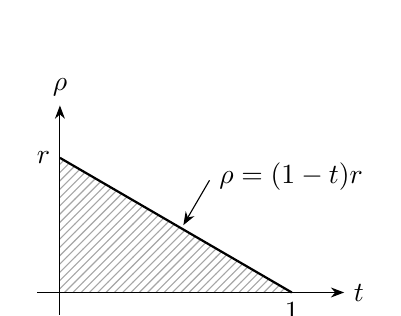
\begin{tikzpicture}[scale=0.95,>=Stealth]
\fill[pattern=north east lines,pattern color=gray!70] (0,0)--(3.1,0)--(0,1.8)--cycle;
\draw[->] (-.3,0)--(3.8,0) node[right]{$t$};
\draw[->] (0,-.3)--(0,2.5) node[above]{$\rho$};
\draw[thick] (0,1.8)--(3.1,0);
\node[left] at (0,1.8){$r$};
\node[below] at (3.1,0){$1$};
\node[right] at (2.0,1.55){$\rho=(1-t)r$};
\draw[->] (2.0,1.5)--(1.65,.9);
\end{tikzpicture}
\end{center}
故上一页最后的积分等于
\[
\frac1{\omega_n r^n}
\int_0^r\int_0^{1-\rho/r}\int_{\partial B(x,\rho)}
|Du(z)|(1-t)^{-n-1}|z-x|\dd S\dd t\dd\rho.
\]
板书旁算：
\[
\begin{aligned}
\int_0^{1-\rho/r}(1-t)^{-n-1}\dd t
&=\left.\frac1n(1-t)^{-n}\right|_0^{1-\rho/r}\\
&=\frac1n\left(\frac{r^n}{\rho^n}-1\right)
\leq\frac1n\frac{r^n}{\rho^n}.
\end{aligned}
\]
因为 $|z-x|=\rho$，上述积分不超过
\[
\begin{aligned}
\frac1{n\omega_n}\int_0^r\int_{\partial B(x,\rho)}
|Du(z)|\,|z-x|^{1-n}\dd S\dd\rho
&=\frac1{n\omega_n}\int_{B(x,r)}
\frac{|Du(z)|}{|z-x|^{n-1}}\dd z.
\end{aligned}
\]
归纳为
\[
\boxed{\frac1{\omega_n r^n}\int_{B(x,r)}|u(x)-u(y)|\dd y
\leq\frac1{n\omega_n}\int_{B(x,r)}
\frac{|Du(z)|}{|z-x|^{n-1}}\dd z.}
\]
\ednote{这里保留较强的“绝对差的平均”估计，它也控制上一页的“与球平均之差”；
后面的两点估计正是使用此式。积分核在 $z=x$ 处的值不影响积分。}


\newpage
\subsection*{Morrey 不等式的证明（续）：上确界估计}
\source{9.30/12}
\proofrating{16（续）}{5}{理解 $p>n$ 如何保证积分核可积，从而得到上确界估计。}
$1^\circ$ 取 $r=1$，则
\[
\begin{aligned}
|u(x)|
&\leq\frac1{\omega_n}\int_{B(x,1)}|u(y)|\dd y
+\frac1{n\omega_n}\int_{B(x,1)}
\frac{|Du(z)|}{|z-x|^{n-1}}\dd z\\
&\leq\frac1{\omega_n}
\left(\int_{\R^n}|u(y)|^p\dd y\right)^{1/p}\omega_n^{\,1-1/p}\\
&\quad+\frac1{n\omega_n}
\left(\int_{\R^n}|Du(z)|^p\dd z\right)^{1/p}
\left(\int_{B(0,1)}\frac1{|z|^{p(n-1)/(p-1)}}\dd z\right)^{1-1/p}\\
&\leq C\|u\|_{W^{1,p}(\R^n)}.
\end{aligned}
\]
这里使用
\[
\frac{p(n-1)}{p-1}<n\quad\Longleftrightarrow\quad p>n.
\]
因此
\[
\|u\|_{L^\infty(\R^n)}
\leq C\|u\|_{W^{1,p}(\R^n)}.
\]

\subsection*{两点估计的开始}
\source{9.30/12 右下、13}
\proofrating{16（续）}{5}{核心：通过两球交集的平均，把两点差转成球平均估计。}
$2^\circ$ 任给 $x,y\in\R^n$，$x\ne y$，记 $r=|x-y|$。对所有 $z\in\R^n$，
\[
|u(x)-u(y)|\leq|u(x)-u(z)|+|u(z)-u(y)|.
\]
于是板书写为
\[
\begin{aligned}
|u(x)-u(y)|
&\leq\frac{C}{|B(x,r)|}\int_{B(x,r)}|u(x)-u(z)|\dd z\\
&\quad+\frac{C}{|B(y,r)|}\int_{B(y,r)}|u(y)-u(z)|\dd z.
\end{aligned}
\]
\ednote{这一步可先在两球的交集 $B(x,r)\cap B(y,r)$ 上对 $z$ 取平均。
因 $r=|x-y|$，交集体积至少为 $\omega_n(r/2)^n$，再扩大积分区域到各自的球，
即得板书中的常数 $C=C(n)$。}

\newpage
\subsection*{Morrey 不等式的证明（续）：Hölder 估计与局部形式}
\source{9.30/13--15 左侧}
\proofrating{16（续）}{5}{掌握尺度 $r^{1-n/p}$ 的来源，并理解局部形式。}
应用球平均估计及 Hölder 不等式，
\[
\begin{aligned}
|u(x)-u(y)|
&\leq\frac{C}{n\omega_n}\int_{B(x,r)}
\frac{|Du(z)|}{|z-x|^{n-1}}\dd z
+\frac{C}{n\omega_n}\int_{B(y,r)}
\frac{|Du(z)|}{|z-y|^{n-1}}\dd z\\
&\leq C\left(\int_{\R^n}|Du(z)|^p\dd z\right)^{1/p}
|x-y|^{1-n/p}.
\end{aligned}
\]
\ednote{两项作相同估计，板书最后的“$+\cdots$”在上式中合并。所用尺度关系为
\[
\left(\int_{B(0,r)}|z|^{-p(n-1)/(p-1)}\dd z\right)^{1-1/p}
=C(n,p)\,r^{\,1-n/p}.
\]
}
因此
\[
[u]_{C^{0,\,1-n/p}(\R^n)}
\leq C\|Du\|_{L^p(\R^n)}.
\]
结合上确界估计，得到 Morrey 不等式。
\ednote{$p=\infty$ 时由线段积分直接得
$|u(x)-u(y)|\leq\|Du\|_\infty|x-y|$，与 $\|u\|_\infty$ 合并即可。
这里 $[\cdot]_{C^{0,\gamma}}$ 表示 Hölder 半范数。}

\textbf{注：局部形式。}设 $n<p<\infty$，$x\in\R^n$，$r_0>0$。则
\[
\boxed{|u(x)-u(y)|
\leq C|x-y|^{1-n/p}
\left(\int_{B(x,\,2|x-y|)}|Du(z)|^p\dd z\right)^{1/p},}
\]
对所有
\[
u\in C^1(B(x,2r_0)),\qquad y\in B(x,r_0)
\]
成立。
\begin{center}
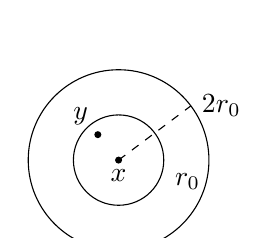
\begin{tikzpicture}[scale=.85]
\draw (0,0) circle(1.35);
\draw (0,0) circle(.675);
\fill (0,0) circle(1.5pt) node[below]{$x$};
\fill (-.31,.38) circle(1.5pt) node[above left]{$y$};
\draw[dashed] (0,0)--(1.08,.81);
\node[right] at (1.1,.81){$2r_0$};
\node[right] at (.7,-.32){$r_0$};
\end{tikzpicture}
\end{center}
\ednote{当 $y=x$ 时结论直接成立。若 $y\ne x$，两球
$B(x,|x-y|)$、$B(y,|x-y|)$ 均包含于 $B(x,2|x-y|)$，
所以前面的证明只需此局部区域内的梯度。}

\newpage
\subsection{区域上的 Morrey 嵌入}
\source{9.30/15 右侧、16}
\proofrating{17}{3}{理解延拓与逼近如何给出 Hölder 连续代表。}
\textbf{定理。}设 $U\subset\R^n$ 为有界开集，$\partial U$ 是 $C^1$ 的，
$n<p<\infty$，$u\in W^{1,p}(U)$。则
\[
u\in C^{0,\,1-n/p}(\overline U),
\]
且
\[
\|u\|_{C^{0,\,1-n/p}(\overline U)}
\leq C\|u\|_{W^{1,p}(U)},\qquad C=C(n,p,U).
\]
\ednote{Sobolev 函数按几乎处处相等视为同一元素；此处指存在上述 Hölder 连续代表。}

\textbf{证明。}存在 $\overline u\in W^{1,p}(\R^n)$，使
\[
\overline u=u\quad\text{于 }U,\qquad
\operatorname{supp}\overline u\text{ 紧},
\qquad
\|\overline u\|_{W^{1,p}(\R^n)}\leq C\|u\|_{W^{1,p}(U)}.
\]
存在 $\{u_m\}_{m=1}^\infty\subset C_c^\infty(\R^n)$，使
\[
u_m\longrightarrow\overline u\quad\text{于 }W^{1,p}(\R^n).
\]
由全空间的 Morrey 不等式，
\[
\|u_m\|_{C^{0,\,1-n/p}(\R^n)}
\leq C\|u_m\|_{W^{1,p}(\R^n)}.
\]
因此
\[
u_m\longrightarrow\overline u\quad\text{于 }C^{0,\,1-n/p}(\R^n).
\]
于是
\[
\begin{aligned}
\|u\|_{C^{0,\,1-n/p}(\overline U)}
&\leq\|\overline u\|_{C^{0,\,1-n/p}(\R^n)}\\
&\leq C\|\overline u\|_{W^{1,p}(\R^n)}
\leq C\|u\|_{W^{1,p}(U)}.
\end{aligned}
\]
\ednote{照片 16 左下估计的右端区域写成 $U$，这里修正为 $\R^n$，
以便与所用的全空间不等式及逼近一致。
对差 $u_m-u_l$ 应用估计可知其在 Hölder 范数下为 Cauchy 列，
其一致极限与 $\overline u$ 几乎处处相等。}

\textbf{零边界值情形。}\source{9.30/17；由前一定理修改得到}
\proofrating{18}{1}{证明可跳过：零延拓后直接应用前面的 Morrey 估计。}
设 $U\subset\R^n$ 为开集，$n<p<\infty$，$u\in W_0^{1,p}(U)$，则同样有
\[
u\in C^{0,\,1-n/p}(\overline U),\qquad
\|u\|_{C^{0,\,1-n/p}(\overline U)}
\leq C\|u\|_{W^{1,p}(U)}.
\]
\ednote{照片 17 将 $W^{1,p}$ 改为 $W_0^{1,p}$，并划去区域的附加要求。
这里可用零延拓和 $C_c^\infty(U)$ 逼近；无需边界光滑性。
板书保留 $C=C(n,p,U)$ 的写法，零延拓论证实际上可取 $C=C(n,p)$。}

\newpage
\subsection{一般的 Sobolev 不等式}
\source{9.30/18}
\proofrating{19}{3}{理解反复使用一阶嵌入：每次提高可积指数并减少一阶导数。}
\textbf{定理。}设 $U\subset\R^n$ 为有界开集，$\partial U$ 是 $C^1$ 的，
$u\in W^{k,p}(U)$。

\textbf{（i）若 $kp<n$，}则 $u\in L^{np/(n-kp)}(U)$，且
\[
\boxed{\|u\|_{L^{np/(n-kp)}(U)}
\leq C\|u\|_{W^{k,p}(U)},\qquad C=C(n,p,k,U).}
\]

\textbf{证明。}对所有多重指标 $\beta$，$|\beta|\leq k-1$，有
\[
D^\beta u\in W^{1,p}(U)\subset L^{np/(n-p)}(U)
\qquad(p<n),
\]
并且
\[
\begin{aligned}
\|D^\beta u\|_{L^{np/(n-p)}(U)}
&\leq C\|D^\beta u\|_{W^{1,p}(U)}\\
&\leq C\|u\|_{W^{k,p}(U)}.
\end{aligned}
\]
因此
\[
u\in W^{k-1,\,np/(n-p)}(U),
\]
且
\[
\|u\|_{W^{k-1,\,np/(n-p)}(U)}
\leq C\|u\|_{W^{k,p}(U)}.
\]
\ednote{照片 18 写到这一轮降阶与提高可积指数。
继续迭代时令 $p_j=np/(n-jp)$，则
$1/p_j=1/p-j/n$。条件 $kp<n$ 保证每轮使用一阶嵌入时的指数小于 $n$；
共 $k$ 轮即得到定理中的 $p_k=np/(n-kp)$。}

\newpage
\subsection*{高阶嵌入：$kp>n$ 的情形（照片所见部分）}
\source{9.30/19}
\proofrating{20}{3}{理解先提高可积性、再对导数用 Morrey；仅评价已录入分支。}
沿用前一定理的区域与函数条件。若 $kp>n$，则存在非负整数 $l$，使
\[
(k-l)p>n\geq(k-l-1)p.
\]
板书接着讨论
\[
\text{\textcircled{1}}\quad n>(k-l-1)p
\]
的情形。对所有多重指标 $\alpha$，$|\alpha|\leq l+1$，有
\[
D^\alpha u\in W^{k-l-1,p}(U)
\subset L^{np/[n-(k-l-1)p]}(U).
\]
因此
\[
u\in W^{l+1,\,np/[n-(k-l-1)p]}(U).
\]
对所有多重指标 $\beta$，$|\beta|\leq l$，有
\[
D^\beta u\in W^{1,\,np/[n-(k-l-1)p]}(U).
\]
注意
\[
\frac{np}{n-(k-l-1)p}>n
\quad\Longleftrightarrow\quad (k-l)p>n.
\]
由 Morrey 嵌入，
\[
D^\beta u\in C^{0,\,k-l-n/p}(\overline U).
\]
所以
\[
\boxed{u\in C^{l,\gamma}(\overline U),\qquad
\gamma=k-l-\frac np.}
\]
\ednote{在本页的严格不等式条件下，$0<\gamma<1$。
若 $k-l-1=0$，上述中间空间就是 $W^{0,p}=L^p$，无需应用正阶嵌入。
本次照片未拍到 $n=(k-l-1)p$ 分支，也未见 $kp=n$ 的单独讨论。
其中等号分支在 10 月 10 日板书中接续，见后文。}

\newpage
\fancyhead[R]{\small 2026 年 10 月 10 日}
\begin{center}
{\LARGE\bfseries 10 月 10 日课堂板书}\\[5pt]
{高阶 Sobolev 嵌入续证、紧嵌入与 Poincaré 不等式}
\end{center}

\subsection*{高阶嵌入：接 9 月 30 日}
\source{10.10/01--02}
\proofrating{20（续）}{3}{区分非整数指数与临界等号分支，掌握任意小的 Hölder 指数损失。}
设 $U\subset\R^n$ 为有界开集，$\partial U$ 是 $C^1$ 的，
$u\in W^{k,p}(U)$，$kp>n$。取非负整数 $l$，使
\[
(k-l)p>n\geq(k-l-1)p.
\]

\textbf{\textcircled{1} 若 $n>(k-l-1)p$，}沿用上次课的推导，令
\[
s=\frac{np}{n-(k-l-1)p}>n.
\]
则 $u\in W^{l+1,s}(U)$；对 $|\beta|\leq l$，
\[
D^\beta u\in W^{1,s}(U)
\subset C^{0,\,1-n/s}(\overline U)
=C^{0,\,k-l-n/p}(\overline U).
\]
因此
\[
\boxed{u\in C^{l,\,k-l-n/p}(\overline U),\qquad 0<k-l-n/p<1.}
\]

\textbf{\textcircled{2} 若 $n=(k-l-1)p$，}则
\[
n>(k-l-2)p,\qquad
u\in W^{l+2,\,np/[n-(k-l-2)p]}(U)=W^{l+2,n}(U).
\]
对 $|\alpha|\leq l+1$，有
\[
D^\alpha u\in W^{1,n}(U)\subset L^q(U),\qquad n<q<\infty.
\]
于是对任意 $n<q<\infty$，
\[
u\in W^{l+1,q}(U),\qquad
D^\beta u\in W^{1,q}(U)\subset C^{0,\,1-n/q}(\overline U)
\quad(|\beta|\leq l).
\]
令 $q=n/(1-\gamma)$，得到
\[
\boxed{u\in C^{l,\gamma}(\overline U),\qquad\text{任意 }0<\gamma<1.}
\]
\ednote{等号分支的结论是所有 $\gamma<1$，不能由这里的临界嵌入直接取 $\gamma=1$。
若推导中 $k-l-2=0$，中间一步仅是 $W^{0,p}=L^p$ 的记号，不需额外使用正阶嵌入。
以上嵌入均有相应的连续范数估计；等号分支的常数还依赖所选 $\gamma$。}

\newpage
\section{紧嵌入}
\subsection*{Ascoli--Arzelà 定理}
\source{10.10/03}
设 $K\subset\R^n$ 是紧集，$\mathcal F\subset C(K)$。则
\[
\boxed{\mathcal F\text{ 列紧}
\quad\Longleftrightarrow\quad
\mathcal F\text{ 一致有界且等度连续}.}
\]
\ednote{板书的“列紧”指：任取 $\mathcal F$ 中的序列，均可选出在 $C(K)$
的一致范数下收敛的子列，极限允许在其闭包中。亦即 $\mathcal F$ 相对紧。}

\subsection{Rellich--Kondrachov 紧嵌入}
\source{10.10/04}
\proofrating{21}{5}{掌握延拓、磨光的一致逼近、Ascoli--Arzelà 定理与对角线选列。}
\textbf{定理。}设 $U\subset\R^n$ 为有界开集，$\partial U$ 是 $C^1$ 的，
$1\leq p<n$。对任意 $1\leq q<p^*=np/(n-p)$，有
\[
\boxed{W^{1,p}(U)\Subset L^q(U).}
\]
\ednote{$X\Subset Y$ 表示紧嵌入：$X$ 中每个有界序列均有在 $Y$ 中收敛的子列。
板书用双重包含号表示此记号。}

\textbf{证明的准备。}固定 $1\leq q<p^*$，设 $\{u_m\}_{m=1}^\infty$
在 $W^{1,p}(U)$ 中有界，即
\[
\sup_m\|u_m\|_{W^{1,p}(U)}<\infty.
\]
取有界开集 $W$，使 $U\Subset W$。由延拓定理可取
$\overline u_m\in W^{1,p}(\R^n)$，满足
\[
\overline u_m=u_m\ \text{a.e. 于 }U,\qquad
\operatorname{supp}\overline u_m\subset W,\qquad
\|\overline u_m\|_{W^{1,p}(\R^n)}
\leq C\|u_m\|_{W^{1,p}(U)}.
\]
因此只须证明延拓后的序列在包含其支撑的固定有界开集 $V$ 上有 $L^q$ 收敛子列。
以下仍将延拓后的函数记为 $u_m$，并取 $W\Subset V$。

令
\[
u_m^\varepsilon=\eta_\varepsilon*u_m.
\]
当 $\varepsilon$ 足够小时，所有 $u_m^\varepsilon$ 的支撑仍包含于 $V$。
下面证明：
\[
\begin{array}{ll}
\text{\textcircled{1}}&u_m^\varepsilon\longrightarrow u_m\text{ 于 }L^q(V),
\quad\varepsilon\to0,\text{ 且关于 }m\text{ 一致};\\[3pt]
\text{\textcircled{2}}&\text{固定 }\varepsilon>0,\quad
\{u_m^\varepsilon\}_m\text{ 一致有界且等度连续}.
\end{array}
\]

\newpage
\subsection*{紧嵌入证明：\textcircled{1} 磨光的一致逼近}
\source{10.10/05、07--09；05 中的证明提纲与后续推导合并}
取 $0<\theta\leq1$，使
\[
\frac1q=\theta+\frac{1-\theta}{p^*}.
\]
由插值不等式及全空间 Sobolev 不等式，
\[
\begin{aligned}
\|u_m^\varepsilon-u_m\|_{L^q(V)}
&\leq\|u_m^\varepsilon-u_m\|_{L^1(V)}^\theta
       \|u_m^\varepsilon-u_m\|_{L^{p^*}(V)}^{1-\theta}\\
&\leq C\|u_m^\varepsilon-u_m\|_{L^1(V)}^\theta.
\end{aligned}
\]
\ednote{后一常数与 $m$ 及足够小的 $\varepsilon$ 无关，因为
$\|u_m^\varepsilon\|_{W^{1,p}(\R^n)}\leq\|u_m\|_{W^{1,p}(\R^n)}$，
而后者一致有界。$q=1$ 时直接取 $\theta=1$。}
只需证 $u_m^\varepsilon\to u_m$ 于 $L^1(V)$，且关于 $m$ 一致。
对 $x\in V$，作变量替换 $z=(y-x)/\varepsilon$，由线段积分得
\[
\begin{aligned}
|u_m^\varepsilon(x)-u_m(x)|
&\leq\int_{B(x,\varepsilon)}\eta_\varepsilon(x-y)
             |u_m(y)-u_m(x)|\dd y\\
&=\int_{B(0,1)}\eta(z)|u_m(x+\varepsilon z)-u_m(x)|\dd z\\
&\leq\varepsilon\int_{B(0,1)}\eta(z)
             \int_0^1|Du_m(x+t\varepsilon z)|\dd t\dd z.
\end{aligned}
\]
在 $x$ 上积分并交换次序，利用平移不改变全空间积分，
\[
\begin{aligned}
\|u_m^\varepsilon-u_m\|_{L^1(V)}
&\leq\varepsilon\int_{B(0,1)}\eta(z)\int_0^1
       \int_{\R^n}|Du_m(x+t\varepsilon z)|\dd x\dd t\dd z\\
&=\varepsilon\|Du_m\|_{L^1(\R^n)}\\
&\leq\varepsilon |V|^{1-1/p}\|Du_m\|_{L^p(\R^n)}
\leq C\varepsilon.
\end{aligned}
\]
于是
\[
\boxed{\sup_m\|u_m^\varepsilon-u_m\|_{L^q(V)}
\leq C\varepsilon^\theta\longrightarrow0.}
\]
\ednote{照片中的线段积分先对光滑函数成立；一般的 $W^{1,p}$ 函数可先作光滑逼近，
在 $L^1$ 平移估计中取极限。换序后把积分区域先扩大到 $\R^n$，
再利用 $Du_m$ 的固定有界支撑，可使板书中的平移换元严格成立。}

\newpage
\subsection*{紧嵌入证明：\textcircled{2} 固定磨光尺度的紧性}
\source{10.10/09--11}
固定足够小的 $\varepsilon>0$。对所有 $x\in\R^n$，
\[
\begin{aligned}
|u_m^\varepsilon(x)|
&=\left|\int_{B(x,\varepsilon)}\eta_\varepsilon(x-y)u_m(y)\dd y\right|\\
&\leq C\varepsilon^{-n}\int_V|u_m(y)|\dd y\\
&\leq C\varepsilon^{-n}|V|^{1-1/p}\|u_m\|_{L^p(V)}
\leq C(\varepsilon),
\end{aligned}
\]
且
\[
\begin{aligned}
|Du_m^\varepsilon(x)|
&=\left|\int_{B(x,\varepsilon)}D\eta_\varepsilon(x-y)u_m(y)\dd y\right|\\
&\leq C\varepsilon^{-n-1}|V|^{1-1/p}\|u_m\|_{L^p(V)}
\leq C(\varepsilon).
\end{aligned}
\]
所以 $\{u_m^\varepsilon\}_m$ 在 $\overline V$ 上一致有界且等度连续。
由 Ascoli--Arzelà 定理，可取子列在 $\overline V$ 上一致收敛，
从而在 $L^q(V)$ 中收敛。

\subsection*{对角线选列与证明结束}
\source{10.10/05--06；与前两步的证明结论接合}
对任意 $\delta>0$，由\textcircled{1}可取 $\varepsilon>0$，使所有 $m$ 均满足
\[
\|u_m^\varepsilon-u_m\|_{L^q(V)}<\frac\delta2.
\]
对该 $\varepsilon$，由\textcircled{2}选取子列，使磨光后的子列在 $L^q(V)$ 中收敛。
对选出的指标 $m_j,m_k$，有
\[
\begin{aligned}
\|u_{m_j}-u_{m_k}\|_{L^q(V)}
&\leq\|u_{m_j}-u_{m_j}^\varepsilon\|_{L^q(V)}
 +\|u_{m_j}^\varepsilon-u_{m_k}^\varepsilon\|_{L^q(V)}\\
&\qquad+\|u_{m_k}^\varepsilon-u_{m_k}\|_{L^q(V)}.
\end{aligned}
\]
因此该子列满足
\[
\limsup_{j,k\to\infty}\|u_{m_j}-u_{m_k}\|_{L^q(V)}\leq\delta.
\]
依次取 $\delta=1,1/2,1/3,\ldots$，逐层选取嵌套子列，再取对角子列，
即得 $L^q(V)$ 中的 Cauchy 列。由完备性得收敛子列，限制到 $U$ 即证。
\ednote{第 $r$ 层子列的尾部距离上极限不超过 $1/r$；对角子列的尾部包含于每个固定层，
故其距离趋于零。这补足了照片中的对角线示意。}

\newpage
\subsection{临界指数的紧嵌入}
\source{10.10/11--12}
\proofrating{22}{3}{用低指数紧性和高指数有界性插值，处理所有有限目标指数。}
\textbf{定理。}设 $U\subset\R^n$ 为有界开集，$\partial U$ 是 $C^1$ 的。
则对任意 $1\leq q<\infty$，
\[
\boxed{W^{1,n}(U)\Subset L^q(U).}
\]

\textbf{证明：$1^\circ$ $n=1$。}设 $\{u_m\}$ 在 $W^{1,1}(U)$ 中有界。
由前述一维嵌入
\[
W^{1,1}(U)\subset C(\overline U),
\]
知 $\{u_m\}$ 一致有界。取 $q_0>q$，从而
$\sup_m\|u_m\|_{L^{q_0}(U)}<\infty$。
\ednote{照片在此使用 $L^1$ 紧性。可将前面紧嵌入证明中的两步直接用于 $L^1$：
一致逼近估计 $\|u_m^\varepsilon-u_m\|_1\leq C\varepsilon$ 和固定尺度的
Ascoli--Arzelà 紧性在一维同样成立，无需 $p<n$。故可先取子列在 $L^1(U)$ 中收敛。}
仍将该子列记为 $\{u_m\}$。若 $q>1$，选取 $0<\theta<1$，使
$1/q=\theta+(1-\theta)/q_0$，则
\[
\begin{aligned}
\|u_{m_j}-u_{m_k}\|_{L^q(U)}
&\leq\|u_{m_j}-u_{m_k}\|_{L^1(U)}^\theta
       \|u_{m_j}-u_{m_k}\|_{L^{q_0}(U)}^{1-\theta}\\
&\leq C\|u_{m_j}-u_{m_k}\|_{L^1(U)}^\theta\longrightarrow0.
\end{aligned}
\]
$q=1$ 已包括在选列步骤中。

\textbf{$2^\circ$ $n>1$。}给定 $1\leq q<\infty$，可取 $1\leq p_0<n$ 充分接近 $n$，使
\[
q<\frac{np_0}{n-p_0}.
\]
由于 $U$ 有界，
\[
W^{1,n}(U)\subset W^{1,p_0}(U)\Subset L^q(U).
\]
第一箭头连续，第二箭头由上一紧嵌入定理给出，故结论成立。

\subsection{在相同指数下的紧嵌入}
\source{10.10/13}
\proofrating{23}{1}{证明可略：直接组合此前的紧嵌入。}
\textbf{定理。}沿用上述区域条件，对任意 $1\leq p<\infty$，
\[
\boxed{W^{1,p}(U)\Subset L^p(U).}
\]
\textbf{证明。}$p<n$ 时有 $p<p^*$，$p=n$ 时由临界定理。
若 $p>n$，由有界性及临界紧嵌入，
\[
W^{1,p}(U)\subset W^{1,n}(U)\Subset L^p(U).
\]

\newpage
\section{其他性质}
\subsection{Poincaré 不等式：减去平均值}
\source{10.10/14；证明在 10 月 12 日接续}
\proofrating{24}{5}{掌握反证归一化、紧性取极限，以及连通性排除非零常数。}
\textbf{定理。}设 $U\subset\R^n$ 为有界、连通开集，$\partial U$ 是 $C^1$ 的，
$1\leq p<\infty$。则存在 $C=C(n,p,U)>0$，使
\[
\boxed{\|u-(u)_U\|_{L^p(U)}\leq C\|Du\|_{L^p(U)},
\qquad u\in W^{1,p}(U),}
\]
其中
\[
(u)_U=\frac1{|U|}\int_Uu(x)\dd x.
\]
\ednote{照片 10.10/14 先陈述有界开集上的形式，10.12/01--02 明确写出“连通”。
这里采用完整条件；否则不同连通分支上的不同常数会构成反例。
这与前面零边界值版本的 Poincaré 不等式分别保留。}

\textbf{反证法的开始。}若不成立，则对每个 $k\in\N$，存在 $u_k\in W^{1,p}(U)$，使
\[
\|u_k-(u_k)_U\|_{L^p(U)}>k\|Du_k\|_{L^p(U)}.
\]
后续归一化与紧性论证见 10 月 12 日板书。

\newpage
\fancyhead[R]{\small 2026 年 10 月 12 日}
\begin{center}
{\LARGE\bfseries 10 月 12 日课堂板书}\\[5pt]
{Poincaré 不等式续证、推广及差商}
\end{center}

\subsection*{平均值型 Poincaré 不等式的证明（接 10 月 10 日）}
\source{10.12/01--03；01--02 为同一板书的先后版本}
\proofrating{24（续）}{5}{归一化使范数固定，紧嵌入使极限仍保有范数，而梯度极限为零。}
沿用上次课的条件：$U$ 有界、连通，$\partial U$ 是 $C^1$ 的，$1\leq p<\infty$。
若不等式不成立，可取
\[
\|u_k-(u_k)_U\|_{L^p(U)}>k\|Du_k\|_{L^p(U)}.
\]
令
\[
v_k=\frac{u_k-(u_k)_U}{\|u_k-(u_k)_U\|_{L^p(U)}}.
\]
则
\[
\|v_k\|_{L^p(U)}=1,\qquad
\int_Uv_k\dd x=0,\qquad
\|Dv_k\|_{L^p(U)}<\frac1k.
\]
于是 $\{v_k\}$ 在 $W^{1,p}(U)$ 中有界。由紧嵌入
\[
W^{1,p}(U)\Subset L^p(U),
\]
可取子列（仍记为 $\{v_k\}$）及 $v\in L^p(U)$，使
\[
v_k\longrightarrow v\quad\text{于 }L^p(U).
\]
因而
\[
\|v\|_{L^p(U)}=1,\qquad\int_Uv\dd x=0.
\]
对任意 $\phi\in C_c^\infty(U)$，$i=1,\ldots,n$，有
\[
\begin{aligned}
-\int_Uv\phi_{x_i}\dd x
&=-\lim_{k\to\infty}\int_Uv_k\phi_{x_i}\dd x\\
&=\lim_{k\to\infty}\int_U(v_k)_{x_i}\phi\dd x=0.
\end{aligned}
\]
所以 $Dv=0$。由 $U$ 连通，$v$ 几乎处处等于某常数 $c$；
再由 $\int_Uv=0$，得 $c=0$，与 $\|v\|_{L^p(U)}=1$ 矛盾。
\ednote{照片最后写到“由连通性，$v=c$ 于 $U$”；这里补出均值为零所导致的矛盾。
$Dv=0$ 推出常数的论证可先在内含小球上磨光，再用连通性将局部常数拼接。}

\newpage
\subsection{用梯度和较低阶积分控制函数}
\source{10.12/04、06--08 左侧；06--07 的重拍部分合并}
\proofrating{25}{3}{区分 $q\geq1$ 的平均值估计与 $0<q<1$ 的反证紧性论证。}
\textbf{定理。}设 $U\subset\R^n$ 为有界、连通开集，$\partial U$ 是 $C^1$ 的，
$1<p<\infty$，$q>0$。则存在 $C=C(n,p,q,U)>0$，使
\[
\boxed{\|u\|_{L^p(U)}\leq C\bigl(\|Du\|_{L^p(U)}+\|u\|_{L^q(U)}\bigr),
\quad u\in W^{1,p}(U)\cap L^q(U).}
\]
\ednote{沿用板书的有限指数约定。$0<q<1$ 时
$\|u\|_{L^q(U)}=(\int_U|u|^q\dd x)^{1/q}$ 仍表示该积分量，虽不满足范数的三角不等式。}

\textbf{证明：$1^\circ$ $q\geq1$。}由平均值型 Poincaré 不等式及 Hölder 不等式，
\[
\begin{aligned}
\|u\|_{L^p(U)}
&\leq\|u-(u)_U\|_{L^p(U)}+\|(u)_U\|_{L^p(U)}\\
&\leq C\|Du\|_{L^p(U)}+|U|^{1/p}|(u)_U|\\
&\leq C\|Du\|_{L^p(U)}+|U|^{1/p-1/q}\|u\|_{L^q(U)}.
\end{aligned}
\]

\textbf{$2^\circ$ $0<q<1$。}若结论不成立，利用齐次性，可对每个 $k\in\N$ 选取
$u_k\in W^{1,p}(U)\cap L^q(U)$，使
\[
1=\|u_k\|_{L^p(U)}
>k\bigl(\|Du_k\|_{L^p(U)}+\|u_k\|_{L^q(U)}\bigr).
\]
于是 $\{u_k\}$ 在 $W^{1,p}(U)$ 中有界。取子列使
\[
u_k\longrightarrow u\quad\text{于 }L^p(U),\qquad
\|u\|_{L^p(U)}=1.
\]
由于 $a,b\geq0$ 时 $(a+b)^q\leq a^q+b^q$，
\[
\begin{aligned}
\int_U|u|^q\dd x
&\leq\int_U|u_k-u|^q\dd x+\int_U|u_k|^q\dd x\\
&\leq |U|^{1-q/p}\|u_k-u\|_{L^p(U)}^q+\|u_k\|_{L^q(U)}^q
\longrightarrow0.
\end{aligned}
\]
故 $u=0$ a.e.，矛盾。
\ednote{照片 08 还给出另一种结束方法：进一步取几乎处处收敛子列，再用 Fatou 引理，
\[
\int_U|u|^q\dd x\leq\liminf_{k\to\infty}\int_U|u_k|^q\dd x=0.
\]
照片中将积分和极限直接交换的写法，
这里按 Fatou 引理理解；无需另假定控制函数。}

\newpage
\subsection{零点集具有正测度时的 Poincaré 不等式}
\source{10.12/05、08 右侧、09--10；重复定理陈述合并}
\proofrating{26}{3}{用零点集的统一测度下界，排除紧性极限为非零常数。}
\textbf{定理。}设 $U=B(0,1)$，$\alpha>0$。则存在 $C=C(n,\alpha)>0$，使得
\[
\boxed{\|u\|_{L^2(U)}\leq C\|Du\|_{L^2(U)}}
\]
对所有满足
\[
u\in H^1(U),\qquad |\{x\in U:u(x)=0\}|\geq\alpha
\]
的函数成立。

\textbf{证明。}若不成立，可归一化选取 $u_k\in H^1(U)$，使
\[
|\{u_k=0\}|\geq\alpha,\qquad
1=\|u_k\|_{L^2(U)}>k\|Du_k\|_{L^2(U)}.
\]
由紧嵌入，存在子列及 $u\in L^2(U)$，使
\[
u_k\longrightarrow u\quad\text{于 }L^2(U),\qquad\|u\|_{L^2(U)}=1.
\]
同前面的弱导数检验，$Du=0$；球连通，故 $u=c$ a.e.。
另一方面，
\[
\alpha c^2
\leq\int_{\{u_k=0\}}c^2\dd x
=\int_{\{u_k=0\}}(u_k-u)^2\dd x
\leq\int_U(u_k-u)^2\dd x\longrightarrow0.
\]
所以 $c=0$，矛盾。

\subsection{球上的尺度形式}
\source{10.12/11}
\proofrating{27}{2}{熟悉换元如何产生半径因子 $r$。}
对任意 $x_0\in\R^n$、$r>0$、$1\leq p<\infty$，有
\[
\boxed{\|u-(u)_{x_0,r}\|_{L^p(B(x_0,r))}
\leq Cr\|Du\|_{L^p(B(x_0,r))},\quad C=C(n,p),}
\]
其中 $u\in W^{1,p}(B(x_0,r))$，
$ (u)_{x_0,r}=|B(x_0,r)|^{-1}\int_{B(x_0,r)}u\dd x$。

\textbf{证明。}令 $v(y)=u(x_0+ry)$，$y\in B(0,1)$。则
\[
(v)_{B(0,1)}=(u)_{x_0,r},\qquad D_yv(y)=rDu(x_0+ry).
\]
对 $v$ 用单位球上的 Poincaré 不等式，换元得
\[
r^{-n/p}\|u-(u)_{x_0,r}\|_{L^p(B(x_0,r))}
\leq C r^{1-n/p}\|Du\|_{L^p(B(x_0,r))},
\]
即得结论。
\ednote{照片在代入单位球不等式后结束；此处写出换元的体积因子，以核对半径的幂次。}

\newpage
\subsection{差商与 Sobolev 弱导数}
\source{10.12/12}
设 $u\in L^1_{\mathrm{loc}}(U)$，$V\Subset U$，$i\in\{1,\ldots,n\}$。
定义第 $i$ 个方向的差商
\[
\boxed{D_i^hu(x)=\frac{u(x+he_i)-u(x)}{h},\qquad x\in V,}
\]
其中 $0<|h|<\operatorname{dist}(V,\partial U)$，$e_i$ 为第 $i$ 个标准基向量。

\textbf{定理。}固定 $V\Subset U$ 及方向 $i$。

\textbf{（i）}设 $1\leq p<\infty$，$u\in W^{1,p}(U)$。则当
\[
0<|h|<\frac12\operatorname{dist}(V,\partial U)
\]
时，
\[
\boxed{\|D_i^hu\|_{L^p(V)}\leq\|u_{x_i}\|_{L^p(U)}.}
\]

\textbf{（ii）}设 $1<p<\infty$，$u\in L^p(U)$。若存在 $C_*>0$，使上述所有 $h$ 均满足
\[
\|D_i^hu\|_{L^p(V)}\leq C_*,
\]
则 $u$ 关于 $x_i$ 在 $V$ 上的弱导数存在，且
\[
\boxed{u_{x_i}\in L^p(V),\qquad\|u_{x_i}\|_{L^p(V)}\leq C_*.}
\]
\ednote{照片（ii）将 $u$ 的空间写成 $L^p(V)$，但差商需用到 $V$ 外的平移值，
因此这里明确取 $u\in L^p(U)$。也可只要求 $u$ 在 $\overline V$ 的某个邻域属于 $L^p$。
逆向结论需要 $p>1$；端点反例见 10 月 14 日。}

\subsection*{证明（i）：线段积分与 Jensen 不等式}
\source{10.12/13--14 左侧}
\proofrating{28}{4}{差商估计是后续椭圆方程正则性证明的基本工具。}
先设 $u$ 光滑。对 $x\in V$，
\[
u(x+he_i)-u(x)=\int_0^1u_{x_i}(x+the_i)h\dd t.
\]
由 Jensen 不等式，
\[
\begin{aligned}
\int_V|D_i^hu(x)|^p\dd x
&\leq\int_V\left(\int_0^1|u_{x_i}(x+the_i)|\dd t\right)^p\dd x\\
&\leq\int_0^1\int_V|u_{x_i}(x+the_i)|^p\dd x\dd t\\
&\leq\int_U|u_{x_i}(x)|^p\dd x.
\end{aligned}
\]
\ednote{因为 $V+the_i\subset U$，最后一步成立。
对一般 $W^{1,p}(U)$ 函数，在包含这些平移点的内部区域作光滑逼近，固定 $h$ 后取极限即可。}

\newpage
\subsection*{证明（ii）的开始：差商分部积分}
\source{10.12/14 右侧、15}
\proofrating{29}{4}{把差商从检验函数移到 $u$，再用弱紧性辨认极限。}
对 $\phi\in C_c^\infty(V)$，当 $|h|$ 足够小时，平移换元给出
\[
\int_Vu(x)\phi(x+he_i)\dd x
=\int_Vu(x-he_i)\phi(x)\dd x.
\]
故
\[
\begin{aligned}
-\int_Vu\phi_{x_i}\dd x
&=-\lim_{h\to0}\int_Vu(x)\frac{\phi(x+he_i)-\phi(x)}h\dd x\\
&=\lim_{h\to0}\int_V\frac{u(x-he_i)-u(x)}{-h}\phi(x)\dd x\\
&=\lim_{h\to0}\int_VD_i^{-h}u(x)\phi(x)\dd x.
\end{aligned}
\]
\ednote{此处可先将 $\phi$ 零延拓；由于 $\operatorname{supp}\phi\Subset V$，
对足够小的 $|h|$，所有相关平移仍在 $V$ 中，换元无边界项。
弱极限的选取及范数估计在 10 月 14 日续证。}

\newpage
\fancyhead[R]{\small 2026 年 10 月 14 日}
\begin{center}
{\LARGE\bfseries 10 月 14 日课堂板书}\\[5pt]
{差商续证、Lipschitz 连续、几乎处处可微与负阶空间}
\end{center}

\subsection*{差商判别（ii）的证明（接 10 月 12 日）}
\source{10.14/01--02 左侧；重复陈述合并}
\proofrating{29（续）}{4}{利用 $L^p$ 的自反性取弱收敛子列，并用检验函数识别弱导数。}
由假设，$\{D_i^{-h}u\}$ 在 $L^p(V)$ 中一致有界。
由于 $1<p<\infty$，可选取 $h_k\to0$ 及 $v_i\in L^p(V)$，使
\[
D_i^{-h_k}u\rightharpoonup v_i\quad\text{于 }L^p(V).
\]
由上次课得到的差商分部积分公式，对任意 $\phi\in C_c^\infty(V)$，
\[
-\int_Vu\phi_{x_i}\dd x
=\lim_{k\to\infty}\int_VD_i^{-h_k}u\,\phi\dd x
=\int_Vv_i\phi\dd x.
\]
故 $u_{x_i}=v_i\in L^p(V)$。再由范数的弱下半连续性，
\[
\|u_{x_i}\|_{L^p(V)}
\leq\liminf_{k\to\infty}\|D_i^{-h_k}u\|_{L^p(V)}\leq C_*.
\]

\subsection*{板书旁记：范数的弱下半连续性}
\source{10.14/02 右侧、03 右缘}
设 $\mathcal X$ 为赋范线性空间，$x_k\rightharpoonup x$ 于 $\mathcal X$，则
\[
\boxed{\|x\|\leq\liminf_{k\to\infty}\|x_k\|.}
\]
若 $x=0$，显然成立。若 $x\ne0$，由 Hahn--Banach 定理，存在
$f\in\mathcal X^*$，使
\[
\|f\|=1,\qquad f(x)=\|x\|.
\]
由于 $f(x_k)\leq\|f\|\|x_k\|=\|x_k\|$，取下极限得到
\[
\|x\|=f(x)=\lim_{k\to\infty}f(x_k)
\leq\liminf_{k\to\infty}\|x_k\|.
\]

\newpage
\subsection*{注：逆向差商判别在 $p=1$ 时不成立}
\source{10.14/03--04 左侧}
令
\[
u(x)=\chi_{(0,1)}(x)=
\begin{cases}
1,&x\in(0,1),\\
0,&x\notin(0,1),
\end{cases}
\qquad V=(-1,1).
\]
则对足够小的非零 $h$，
\[
\begin{aligned}
\int_{-1}^1|D^hu(x)|\dd x
&=\frac1{|h|}\int_{-1}^1|u(x+h)-u(x)|\dd x\\
&=\frac1{|h|}\int_{-1}^1
       |\chi_{(-h,1-h)}(x)-\chi_{(0,1)}(x)|\dd x
\leq2.
\end{aligned}
\]
\ednote{可将 $u$ 看作定义在 $U=(-2,2)$ 上。虽然差商在 $L^1(V)$ 中一致有界，
但 $u$ 在 $0$ 处有跳跃，其分布导数在 $V$ 内是 Dirac 测度 $\delta_0$，
不能由 $L^1(V)$ 函数表示。这明确给出了板书“$p=1$ 不成立”的原因。}

\subsection*{注：平边界附近的切向差商}
\source{10.14/04}
令
\[
U=B(0,1)\cap\{x_n>0\},\qquad
V=B(0,\tfrac12)\cap\{x_n>0\}.
\]
对于切向方向 $i=1,\ldots,n-1$，当 $0<|h|<1/2$ 时，
$D_i^hu(x)$ 在 $x\in V$ 上有定义。
\begin{center}
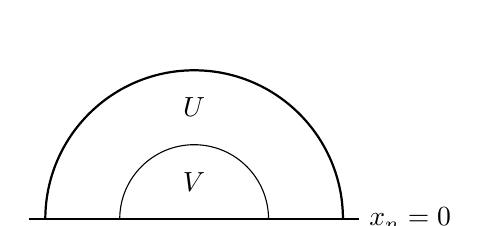
\begin{tikzpicture}[scale=1.05]
\draw[thick] (-2,0)--(2,0);
\draw[thick] (1.8,0) arc[start angle=0,end angle=180,radius=1.8];
\draw (0.9,0) arc[start angle=0,end angle=180,radius=0.9];
\node at (0,.45){$V$};
\node at (0,1.35){$U$};
\node[right] at (2,0){$x_n=0$};
\end{tikzpicture}
\end{center}
在此半球设置中，对 $0<|h|<1/4$，正向估计仍成立：
\[
\|D_i^hu\|_{L^p(V)}\leq\|u_{x_i}\|_{L^p(U)},
\qquad u\in W^{1,p}(U),\quad1\leq p<\infty.
\]
若 $1<p<\infty$，$u\in L^p(U)$，且切向差商在 $L^p(V)$ 中一致有界，
则同样得到切向弱导数 $u_{x_i}\in L^p(V)$ 及相应范数界。
\ednote{此处 $V$ 接触平边界，并非 $V\Subset U$；关键是切向平移线段仍留在 $U$ 内。
板书的 $1/4$ 是方便选取的步长上界。图按照片的半球示意重绘。}

\newpage
\subsection{Lipschitz 连续与一阶有界弱导数}
\source{10.14/05--07}
\proofrating{30}{4}{正向磨光后沿线段积分；逆向以有界差商及弱星收敛构造弱导数。}
\textbf{定理。}设 $U\subset\R^n$ 为有界开集，$\partial U$ 是 $C^1$ 的。
对于 $u:U\to\R$，
\[
\boxed{u\in C^{0,1}(\overline U)
\quad\Longleftrightarrow\quad u\in W^{1,\infty}(U).}
\]
\ednote{右侧按几乎处处相等理解，结论指存在左侧的 Lipschitz 连续代表。
由延拓定理及 Lipschitz 函数的延拓，可按板书先考虑定义在 $\R^n$ 上且有紧支撑的函数。
区域上的 Lipschitz 常数可以依赖 $U$；全空间线段估计见下式。}

\textbf{证明：$1^\circ$ 设 $u\in W^{1,\infty}(\R^n)$。}
取其连续代表，令 $u^\varepsilon=\eta_\varepsilon*u$。由磨光性质，
\[
u^\varepsilon\longrightarrow u\quad\text{一致于 }\R^n,\qquad
\|Du^\varepsilon\|_{L^\infty(\R^n)}
\leq\|Du\|_{L^\infty(\R^n)}.
\]
对 $x,y\in\R^n$，
\[
\begin{aligned}
|u^\varepsilon(x)-u^\varepsilon(y)|
&=\left|\int_0^1Du^\varepsilon(tx+(1-t)y)\cdot(x-y)\dd t\right|\\
&\leq\int_0^1|Du^\varepsilon(tx+(1-t)y)|\dd t\,|x-y|\\
&\leq\|Du\|_{L^\infty(\R^n)}|x-y|.
\end{aligned}
\]
令 $\varepsilon\to0$，得
\[
|u(x)-u(y)|\leq\|Du\|_{L^\infty(\R^n)}|x-y|.
\]
\ednote{板书线段积分处的第一个等号应先用于 $u^\varepsilon$，且绝对值须置于整个积分外；
这里已修正。紧支撑的连续代表一致连续，所以其磨光一致收敛。
也可直接在几乎处处收敛点上取极限，再延拓得到同一 Lipschitz 代表。}

\newpage
\subsection*{Lipschitz 等价定理的证明（续）}
\source{10.14/06--07 右侧}
\textbf{$2^\circ$ 设 $u$ 是 Lipschitz 连续函数。}记
\[
\operatorname{Lip}(u)=\sup_{x\ne y}\frac{|u(x)-u(y)|}{|x-y|}.
\]
则对任意 $x\in\R^n$、$h\ne0$，
\[
\left|\frac{u(x-he_i)-u(x)}{-h}\right|
\leq\operatorname{Lip}(u),
\]
从而
\[
\|D_i^{-h}u\|_{L^\infty(\R^n)}\leq\operatorname{Lip}(u).
\]
可取 $h_k\to0$ 及 $v_i\in L^\infty(\R^n)$，使
\[
D_i^{-h_k}u\overset{*}{\rightharpoonup}v_i
\quad\text{于 }L^\infty(\R^n).
\]
因此对所有 $\phi\in C_c^\infty(\R^n)$，
\[
\begin{aligned}
-\int_{\R^n}u\phi_{x_i}\dd x
&=\lim_{k\to\infty}\int_{\R^n}D_i^{-h_k}u\,\phi\dd x\\
&=\int_{\R^n}v_i\phi\dd x.
\end{aligned}
\]
故 $u_{x_i}=v_i\in L^\infty$。结合 $u$ 的有界性即得 $u\in W^{1,\infty}$。
\ednote{本步的收敛为弱星收敛，不能照搬 $1<p<\infty$ 时的自反性。
可由有界集的弱星紧性及 $L^1(\R^n)$ 的可分性取出该子列。
有界区域上 Lipschitz 函数自动有界，延拓到全空间后再乘截断函数可满足板书的紧支撑约定。}

\subsection*{板书旁记}
\source{10.14/07 下方；10.14/11 为可微性推论的补拍}
\[
W^{1,\infty}(U)\subset L^\infty(U).
\]
Lipschitz 连续函数的几乎处处可微性由下面的定理得到。

\newpage
\subsection{几乎处处可微}
\source{10.14/08--11}
\proofrating{31}{5}{将一阶余项代入局部 Morrey 估计，再用梯度的 Lebesgue 点性质得到小 $o$。}
\textbf{定理。}设 $U\subset\R^n$ 为开集，$n<p\leq\infty$，
$u\in W^{1,p}_{\mathrm{loc}}(U)$。则 $u$ 在 $U$ 上几乎处处可微，
且其古典意义下的梯度与弱梯度几乎处处相等。
\ednote{这里始终选用局部 Morrey 嵌入所给出的连续代表。}

\textbf{证明目标。}对于几乎所有 $x\in U$，证明
\[
u(y)-u(x)-Du(x)\cdot(y-x)=o(|y-x|),\qquad y\to x,
\]
其中 $Du=(u_{x_1},\ldots,u_{x_n})$ 为弱梯度。

\textbf{$1^\circ$ $n<p<\infty$。}由 Lebesgue 微分定理，几乎处处有
\[
\lim_{r\to0}\frac1{|B(x,r)|}\int_{B(x,r)}|Du(z)-Du(x)|^p\dd z=0.
\tag{$*$}
\]
固定满足 $(*)$ 的 $x$。取 $r_0>0$，使 $B(x,r_0)\Subset U$，令
\[
v(y)=u(y)-u(x)-Du(x)\cdot(y-x),\qquad y\in B(x,r_0).
\]
则 $v\in W^{1,p}(B(x,r_0))$，$v(x)=0$，且
\[
Dv(z)=Du(z)-Du(x).
\]
对于 $y\in B(x,r_0/2)$，记 $r=|y-x|>0$。由局部 Morrey 估计，
\[
\begin{aligned}
|v(y)-v(x)|
&\leq Cr^{1-n/p}\left(\int_{B(x,2r)}|Dv(z)|^p\dd z\right)^{1/p}\\
&\leq C|y-x|\left(\frac1{|B(x,2r)|}
       \int_{B(x,2r)}|Du(z)-Du(x)|^p\dd z\right)^{1/p}.
\end{aligned}
\]
由 $(*)$，括号内趋于零，所以
\[
|u(y)-u(x)-Du(x)\cdot(y-x)|=o(|y-x|).
\]
\ednote{前面的局部 Morrey 估计先对光滑函数写出；用局部光滑逼近并取连续代表后，
可用于本处的 Sobolev 函数。半径 $2r$ 的球在 $r<r_0/2$ 时包含于 $B(x,r_0)$。}

\textbf{$2^\circ$ $p=\infty$。}任取 $n<q<\infty$，则
\[
W^{1,\infty}_{\mathrm{loc}}(U)\subset W^{1,q}_{\mathrm{loc}}(U),
\]
故由 $1^\circ$ 得到结论。

\textbf{推论（Rademacher 定理）。}Lipschitz 连续函数几乎处处可微。
\ednote{照片 11 左侧写出了
$u\in C^{0,1}(U)\Rightarrow u\in W^{1,\infty}_{\mathrm{loc}}(U)
\Rightarrow u$ 几乎处处可微；这里将其与上述定理合并。}

\newpage
\section{负阶 Sobolev 空间}
\subsection{\texorpdfstring{$H^{-1}(U)$ 的定义与自然嵌入}{负一阶空间的定义与自然嵌入}}
\source{10.14/12 左侧及中部；左侧被遮挡的记号据相邻板书核对}
定义
\[
H^{-1}(U)=\bigl(H_0^1(U)\bigr)^*.
\]
采用 Hilbert 内积及其对应范数
\[
(u,v)_{H_0^1(U)}=\int_U(uv+Du\cdot Dv)\dd x,\qquad
\|u\|_{H_0^1(U)}=\left(\int_U(|u|^2+|Du|^2)\dd x\right)^{1/2}.
\]
\ednote{此处明确使用完整的 $H^1$ 范数，使其与后面板书中的 Riesz 表示式和精确范数公式一致。}
对 $f\in L^2(U)$，定义
\[
\langle T_f,v\rangle=\int_Ufv\dd x,\qquad v\in H_0^1(U).
\]
由 Cauchy--Schwarz 不等式，
\[
|\langle T_f,v\rangle|
\leq\|f\|_{L^2(U)}\|v\|_{L^2(U)}
\leq\|f\|_{L^2(U)}\|v\|_{H_0^1(U)}.
\]
所以
\[
T_f\in H^{-1}(U),\qquad
\|T_f\|_{H^{-1}(U)}\leq\|f\|_{L^2(U)}.
\]
由映射 $f\mapsto T_f$，可将 $L^2(U)$ 连续嵌入 $H^{-1}(U)$，即
\[
H_0^1(U)\subset L^2(U)\subset H^{-1}(U).
\]
\ednote{该映射是单射：若 $T_f=0$，对 $C_c^\infty(U)$ 检验即得 $f=0$ a.e.。
在本课此前使用的有界光滑区域上，第一嵌入还是紧的；
照片以 $\mathcal X\Subset\mathcal H\subset\mathcal X^*$ 作了概括。}

\newpage
\subsection{\texorpdfstring{$H^{-1}$ 元素的表示定理}{负一阶空间元素的表示定理}}
\source{10.14/13；14 为证明开头}
\proofrating{32}{3}{理解负阶元素如何写成 $L^2$ 函数及其分布导数的组合。}
\textbf{定理。}设 $f\in H^{-1}(U)$。

\textbf{（i）}存在 $f^0,f^1,\ldots,f^n\in L^2(U)$，使
\[
\boxed{\langle f,v\rangle
=\int_U\left(f^0v+\sum_{i=1}^nf^iv_{x_i}\right)\dd x,
\qquad v\in H_0^1(U).}
\tag{$\diamond$}
\]
当 $(\diamond)$ 成立时，记
\[
f=f^0-\sum_{i=1}^n(f^i)_{x_i}.
\]
\ednote{上式中的导数是分布导数；$f^i$ 只要求属于 $L^2$，不要求其弱导数也在 $L^2$ 中。}

\textbf{（ii）}在上述范数约定下，
\[
\boxed{\|f\|_{H^{-1}(U)}
=\inf\left\{\left(\int_U\sum_{i=0}^n|f^i|^2\dd x\right)^{1/2}
\,\middle|\,
\begin{gathered}
f^0,\ldots,f^n\in L^2(U),\\
\text{$(\diamond)$ 成立}
\end{gathered}\right\}.}
\]

\textbf{证明（i）的开始。}由 Riesz 表示定理，存在 $w\in H_0^1(U)$，使
\[
\begin{aligned}
\langle f,v\rangle
&=(w,v)_{H_0^1(U)}\\
&=\int_U(wv+Dw\cdot Dv)\dd x,
\qquad v\in H_0^1(U).
\end{aligned}
\]
\ednote{照片 14 的证明写到此等式。取 $f^0=w$、$f^i=w_{x_i}$ 即给出（i）所需的表示。
10 月 14 日照片未提供（ii）的续证；其完整证明已接录于后面的本周板书。}

\newpage
\fancyhead[R]{\small 本周板书（10 月 23 日提供）}
\begin{center}
{\LARGE\bfseries 本周课堂板书（一）}\\[5pt]
{2026 年 10 月 23 日提供：负阶空间、分布与椭圆方程}
\end{center}
\ednote{本批为 10 月 19--23 日当周的板书照片，未注明每次上课的确切日期。
以下按文件名顺序编号为“本周/01--28”；本部分对应 01--11，后半部分对应 12--28。
重拍的定理和推导合并录入。}

\subsection*{表示定理的续证（接 10 月 14 日）}
\source{本周/01--02}
\proofrating{32（续）}{3}{用 Riesz 表示取到下确界，再估计任意一组表示系数。}
沿用前文完整的 $H_0^1(U)$ 范数。由 Riesz 表示定理，存在唯一的
$w\in H_0^1(U)$，使
\[
\langle f,v\rangle=(w,v)_{H_0^1(U)}
=\int_U\left(wv+\sum_{i=1}^nw_{x_i}v_{x_i}\right)\dd x,
\qquad v\in H_0^1(U),
\]
并且
\[
\|f\|_{H^{-1}(U)}=\|w\|_{H_0^1(U)}
=\left(\int_U\bigl(|w|^2+|Dw|^2\bigr)\dd x\right)^{1/2}.
\]
取 $f^0=w$、$f^i=w_{x_i}$（$1\leq i\leq n$），则
\[
f=f^0-\sum_{i=1}^n(f^i)_{x_i},\qquad
\left(\int_U\sum_{i=0}^n|f^i|^2\dd x\right)^{1/2}
=\|f\|_{H^{-1}(U)}.
\]

另一方面，对任意满足同一表示式的 $g^0,\ldots,g^n\in L^2(U)$，
由 Cauchy--Schwarz 不等式，
\[
\begin{aligned}
|\langle f,v\rangle|
&=\left|\int_U\left(g^0v+\sum_{i=1}^ng^iv_{x_i}\right)\dd x\right|\\
&\leq\int_U\left(\sum_{i=0}^n|g^i|^2\right)^{1/2}
               \bigl(|v|^2+|Dv|^2\bigr)^{1/2}\dd x\\
&\leq\left(\int_U\sum_{i=0}^n|g^i|^2\dd x\right)^{1/2}
       \|v\|_{H_0^1(U)}.
\end{aligned}
\]
在 $\|v\|_{H_0^1(U)}\leq1$ 上取上确界，得到
\[
\|f\|_{H^{-1}(U)}
\leq\left(\int_U\sum_{i=0}^n|g^i|^2\dd x\right)^{1/2}.
\]
结合前面的特定表示，得到定理（ii），且下确界由
$(w,w_{x_1},\ldots,w_{x_n})$ 取得。

\newpage
\section{分布与分布导数}
\subsection{试验函数空间与分布}
\source{本周/03--04}
\textbf{试验函数的收敛。}设 $\varphi_j,\varphi\in C_c^\infty(U)$。
称 $\varphi_j\to\varphi$ 于试验函数空间 $\mathcal D(U)$，若：
\begin{enumerate}
\item 存在固定的紧集 $K\Subset U$，使所有 $j$ 都满足
\[
\operatorname{supp}\varphi_j\subset K,\qquad
\operatorname{supp}\varphi\subset K;
\]
\item 对每个多重指标 $\alpha$，均有
\[
\max_{x\in K}|D^\alpha\varphi_j(x)-D^\alpha\varphi(x)|\longrightarrow0.
\]
\end{enumerate}
将 $C_c^\infty(U)$ 配以上述收敛方式，记为 $\mathcal D(U)$。

\textbf{定义。}设 $T$ 是 $\mathcal D(U)$ 上的线性泛函。若
\[
\varphi_j\longrightarrow\varphi\text{ 于 }\mathcal D(U)
\quad\Longrightarrow\quad
\langle T,\varphi_j\rangle\longrightarrow\langle T,\varphi\rangle,
\]
则称 $T$ 为 $U$ 上的一个\textbf{分布}。全体分布记为 $\mathcal D'(U)$。

\textbf{例 1：局部可积函数。}若 $f\in L^1_{\mathrm{loc}}(U)$，定义
\[
\langle T_f,\varphi\rangle=\int_Uf(x)\varphi(x)\dd x,
\qquad\varphi\in\mathcal D(U).
\]
则 $T_f\in\mathcal D'(U)$。
\ednote{共同紧支撑保证
$|\langle T_f,\varphi_j-\varphi\rangle|
\leq\|f\|_{L^1(K)}\|\varphi_j-\varphi\|_{L^\infty(K)}\to0$。
因此可将局部可积函数与它产生的分布相认，后文通常仍写作 $f$。}

\textbf{例 2：Dirac 分布。}在 $U=\R$ 上定义
\[
\boxed{\langle\delta,\varphi\rangle=\varphi(0),\qquad
\varphi\in\mathcal D(\R).}
\]
这是 $\mathcal D(\R)$ 上的连续线性泛函，所以 $\delta\in\mathcal D'(\R)$。

\newpage
\subsection{分布导数与阶跃函数}
\source{本周/05}
设 $T\in\mathcal D'(U)$，$\alpha$ 为任意多重指标，定义
\[
\boxed{\langle D^\alpha T,\varphi\rangle
=(-1)^{|\alpha|}\langle T,D^\alpha\varphi\rangle,
\qquad\varphi\in\mathcal D(U).}
\]
因 $D^\alpha\varphi_j\to D^\alpha\varphi$ 于 $\mathcal D(U)$，故
$D^\alpha T$ 仍为分布。
若 $T$ 由 $f\in L^1_{\mathrm{loc}}(U)$ 产生，则
\[
\langle D^\alpha f,\varphi\rangle
=(-1)^{|\alpha|}\int_UfD^\alpha\varphi\dd x.
\]

\textbf{例：阶跃函数的导数。}令
\[
u(x)=\begin{cases}0,&x<0,\\1,&x>0.\end{cases}
\]
则对 $\varphi\in\mathcal D(\R)$，
\[
\langle u',\varphi\rangle
=-\langle u,\varphi'\rangle
=-\int_0^\infty\varphi'(x)\dd x
=\varphi(0)=\langle\delta,\varphi\rangle.
\]
因此 $u'=\delta$（分布意义）。
\ednote{$u(0)$ 的取值不影响它作为局部可积函数所确定的分布。}

\subsection{负阶空间表示式的分布意义及逆向结论}
\source{本周/06--07}
\proofrating{33}{2}{分部积分的定义确定符号，范数估计与稠密性给出延拓。}
若 $f\in H^{-1}(U)$ 的表示系数为 $f^0,\ldots,f^n\in L^2(U)$，则
对 $\varphi\in\mathcal D(U)$，
\[
\begin{aligned}
\langle f,\varphi\rangle
&=\int_U\left(f^0\varphi+\sum_{i=1}^nf^i\varphi_{x_i}\right)\dd x\\
&=\langle f^0,\varphi\rangle
  -\sum_{i=1}^n\langle(f^i)_{x_i},\varphi\rangle.
\end{aligned}
\]
这正是 $f=f^0-\sum_i(f^i)_{x_i}$ 在 $\mathcal D'(U)$ 中的含义。

反之，任何具有上述形式的分布都满足
\[
|\langle f,\varphi\rangle|
\leq\left(\int_U\sum_{i=0}^n|f^i|^2\dd x\right)^{1/2}
\|\varphi\|_{H_0^1(U)}.
\]
由 $C_c^\infty(U)$ 在 $H_0^1(U)$ 中稠密，$f$ 唯一延拓为
$H_0^1(U)$ 上的连续线性泛函，即 $f\in H^{-1}(U)$。

\newpage
\section{二阶椭圆方程}
\subsection{散度型与非散度型算子}
\source{本周/08、11}
设 $U\subset\R^n$ 为有界开集，考虑齐次 Dirichlet 边值问题
\[
\begin{cases}
Lu=f,&\text{于 }U,\\
u=0,&\text{于 }\partial U.
\end{cases}
\]
板书列出两类二阶线性算子：

\textbf{散度型：}
\[
\boxed{Lu=-\sum_{i,j=1}^n\bigl(a^{ij}(x)u_{x_i}\bigr)_{x_j}
       +\sum_{i=1}^nb^i(x)u_{x_i}+c(x)u.}
\]
\textbf{非散度型：}
\[
\boxed{Lu=-\sum_{i,j=1}^na^{ij}(x)u_{x_ix_j}
       +\sum_{i=1}^nb^i(x)u_{x_i}+c(x)u.}
\]
记 $A(x)=(a^{ij}(x))_{n\times n}$，板书约定 $a^{ij}=a^{ji}$。
\ednote{变系数时，这两式一般表示不同的算子。若系数可微，展开散度型的主部还会产生
$-\sum_{i,j}(a^{ij})_{x_j}u_{x_i}$。
后续只讨论散度型算子的弱解与能量估计；各系数属于 $L^\infty(U)$ 即可，不要求其具有古典导数。}

\subsection*{后续能量估计所用的一致椭圆性}
\ednote{本批照片没有完整拍到一致椭圆性条件的独立陈述，但能量估计中明确使用了常数
$\theta>0$。为明确其前提，在这里补记：存在 $\theta>0$，使对几乎处处的 $x\in U$ 及所有
$\xi\in\R^n$，}
\[
\boxed{\sum_{i,j=1}^na^{ij}(x)\xi_i\xi_j\geq\theta|\xi|^2.}
\]
\ednote{系数矩阵的对称性本身不蕴含这一下界；下文均在该一致椭圆性条件下进行。}

\subsection*{各阶项的物理解释}
\source{本周/11}
\[
\underbrace{-\sum_{i,j}(a^{ij}u_{x_i})_{x_j}}_{\text{扩散}}
\; +\;
\underbrace{\sum_i b^iu_{x_i}}_{\text{输运}}
\; +\;
\underbrace{cu}_{\text{反应}}
\; =\; f.
\]

\newpage
\subsection{热流的稳态模型}
\source{本周/09--11}
设 $u$ 表示温度，$F$ 表示热流密度。在无内部热源的稳态情形，
对任意光滑子区域 $V\Subset U$，流出边界的净热量为零：
\[
\int_{\partial V}F\cdot\nu\dd S=0,
\]
其中 $\nu$ 为 $\partial V$ 的单位外法向量。由散度定理，
\[
\int_V\operatorname{div}F\dd x=0.
\]
由于 $V$ 任意，得到 $\operatorname{div}F=0$。

\begin{center}
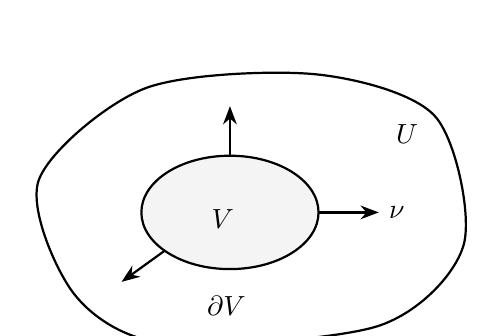
\begin{tikzpicture}[scale=.9,>=Stealth]
\draw[thick] plot[smooth cycle] coordinates
{(0,0) (1.3,-.7) (4.3,-.45) (5.5,.7) (5.1,2.5) (3.4,3.1) (1,2.9) (-.5,1.6)};
\node at (4.7,2.25) {$U$};
\draw[thick,fill=gray!9] (2.2,1.15) ellipse (1.25 and .8);
\node at (2.1,1.05) {$V$};
\draw[->,thick] (3.45,1.15)--(4.3,1.15) node[right] {$\nu$};
\draw[->,thick] (2.2,1.95)--(2.2,2.65);
\draw[->,thick] (1.28,.61)--(.67,.17);
\node at (2.15,-.17) {$\partial V$};
\end{tikzpicture}
\end{center}

\textbf{各向同性介质。}热传导关系为 $F=-aDu$，故
\[
-\operatorname{div}(aDu)=0.
\]
当 $a>0$ 为常数时，化为 $-\Delta u=0$。
\ednote{照片从 $F=-aDu$ 直接写到 $-\Delta u=0$，此处补明 $a$ 为正常数的条件。
若 $a=a(x)$，则保留散度形式。以上推导先在足够光滑的情形理解。}

\textbf{各向异性介质。}更一般地，令
\[
F=-ADu,\qquad F\cdot Du=-ADu\cdot Du\leq0.
\]
此时稳态方程的主部为 $-\operatorname{div}(ADu)=0$。
\ednote{在前述对称性约定下，该矩阵记号与 $-\sum_{i,j}(a^{ij}u_{x_i})_{x_j}$ 一致。}

\newpage
\begin{center}
{\LARGE\bfseries 本周课堂板书（二）}\\[5pt]
{弱解、能量估计与存在性}
\end{center}
\subsection{齐次 Dirichlet 问题的弱解}
\source{本周/12--14}
设 $a^{ij},b^i,c\in L^\infty(U)$，$L$ 为上述散度型算子。定义双线性型
\[
\boxed{B[u,v]=\int_U\left(
\sum_{i,j=1}^na^{ij}u_{x_i}v_{x_j}
+\sum_{i=1}^nb^iu_{x_i}v+cuv\right)\dd x.}
\]
\textbf{定义（$f\in L^2(U)$）。}若 $u\in H_0^1(U)$ 且
\[
B[u,v]=\int_Ufv\dd x,\qquad\forall v\in H_0^1(U),
\]
则称 $u$ 为
\[
Lu=f\text{ 于 }U,\qquad u=0\text{ 于 }\partial U
\]
的一个弱解。
\ednote{将光滑方程乘以检验函数并对散度项分部积分，即得到上述等式。
弱解的边界条件由 $u\in H_0^1(U)$ 表达；在可用迹定理的区域上等价于 $Tu=0$。}

\textbf{推广（$f\in H^{-1}(U)$）。}若 $u\in H_0^1(U)$ 满足
\[
\boxed{B[u,v]=\langle f,v\rangle,\qquad\forall v\in H_0^1(U),}
\]
则仍称其为弱解。特别地，若
\[
f=f^0-\sum_{i=1}^n(f^i)_{x_i},\qquad f^0,\ldots,f^n\in L^2(U),
\]
右侧就是
\[
\langle f,v\rangle
=\int_U\left(f^0v+\sum_{i=1}^nf^iv_{x_i}\right)\dd x.
\]

\subsection*{非齐次边界条件}
\source{本周/14--17}
设 $U$ 为有界 $C^1$ 区域。称 $u\in H^1(U)$ 为
$Lu=f$、$u=g$ 于 $\partial U$ 的弱解，若
\[
B[u,v]=\langle f,v\rangle\quad\forall v\in H_0^1(U),\qquad Tu=g.
\]
这里 $T$ 为迹算子。

\newpage
\subsection{通过提升边界数据化为齐次问题}
\source{本周/15--17}
设有 $w\in H^1(U)$ 满足 $Tw=g$。令
\[
\widetilde u=u-w.
\]
则 $T\widetilde u=0$，从而 $\widetilde u\in H_0^1(U)$，并且
\[
\begin{cases}
L\widetilde u=f-Lw=:\widetilde f,&\text{于 }U,\\
\widetilde u=0,&\text{于 }\partial U.
\end{cases}
\]
\ednote{这一步以边界数据确有 $H^1$ 提升为前提，即 $g$ 属于迹空间。
在本处 $C^1$ 区域上，通常写作 $g\in H^{1/2}(\partial U)$。}

板书先取 $f\in L^2(U)$，将新的右端项写成
\[
\begin{aligned}
\widetilde f
&=f+\sum_{i,j=1}^n(a^{ij}w_{x_i})_{x_j}
     -\sum_{i=1}^nb^iw_{x_i}-cw\\
&=\left(f-\sum_{i=1}^nb^iw_{x_i}-cw\right)
  -\sum_{j=1}^n\left(-\sum_{i=1}^na^{ij}w_{x_i}\right)_{x_j}.
\end{aligned}
\]
即
\[
\widetilde f=g^0-\sum_{j=1}^n(g^j)_{x_j},\qquad
\begin{cases}
g^0=f-\displaystyle\sum_i b^iw_{x_i}-cw,\\[3pt]
g^j=-\displaystyle\sum_i a^{ij}w_{x_i},\quad 1\leq j\leq n.
\end{cases}
\]
由于系数有界、$w\in H^1(U)$，所有 $g^j$ 都属于 $L^2(U)$。
根据前面的表示结论，$\widetilde f\in H^{-1}(U)$。

因此，只要研究齐次 Dirichlet 问题的 $H^{-1}$ 右端项，就可同时处理上述非齐次边界问题。
\ednote{若原来已有 $f\in H^{-1}(U)$，仍可直接定义
$\langle\widetilde f,v\rangle=\langle f,v\rangle-B[w,v]$。
由系数有界性，$|B[w,v]|\leq C\|w\|_{H^1(U)}\|v\|_{H_0^1(U)}$，
故同样有 $\widetilde f\in H^{-1}(U)$。}

\newpage
\subsection{Lax--Milgram 定理与能量估计的陈述}
\source{本周/18--19}
\textbf{Lax--Milgram 定理。}设 $H$ 为实 Hilbert 空间，$B:H\times H\to\R$
为双线性型，并存在常数 $\alpha,\beta>0$，使
\[
|B[u,v]|\leq\alpha\|u\|_H\|v\|_H,\qquad\forall u,v\in H,
\]
\[
B[u,u]\geq\beta\|u\|_H^2,\qquad\forall u\in H.
\]
则对任意 $f\in H^*$，存在唯一的 $u\in H$，满足
\[
\boxed{B[u,v]=\langle f,v\rangle,\qquad\forall v\in H.}
\]
\ednote{照片给出定理陈述，没有拍到证明；$B$ 不要求对称。}

\textbf{能量估计。}对本节的散度型椭圆算子及双线性型 $B$，
存在常数 $\alpha,\beta>0$、$\gamma\geq0$，使
\[
\boxed{|B[u,v]|\leq\alpha\|u\|_{H_0^1(U)}\|v\|_{H_0^1(U)},}
\tag{E1}
\]
\[
\boxed{\beta\|u\|_{H_0^1(U)}^2
\leq B[u,u]+\gamma\|u\|_{L^2(U)}^2,}
\tag{E2}
\]
其中 $u,v\in H_0^1(U)$。
\ednote{照片把三个常数都记为正数；允许 $\gamma=0$ 便于包含后面的特殊例子。
需要正数时可将它增大。常数依赖区域、一致椭圆性常数和系数的 $L^\infty$ 范数。}

\proofrating{34}{3}{有界性用 Cauchy--Schwarz；下界用一致椭圆性、Young 与 Poincaré 不等式。}
\textbf{（E1）的证明。}记
\[
M_a=\sum_{i,j}\|a^{ij}\|_{L^\infty(U)},\qquad
M_b=\sum_i\|b^i\|_{L^\infty(U)},\qquad
M_c=\|c\|_{L^\infty(U)}.
\]
则
\[
\begin{aligned}
|B[u,v]|&\leq M_a\int_U|Du||Dv|\dd x
 +M_b\int_U|Du||v|\dd x+M_c\int_U|u||v|\dd x\\
&\leq M_a\|Du\|_2\|Dv\|_2
 +M_b\|Du\|_2\|v\|_2+M_c\|u\|_2\|v\|_2\\
&\leq(M_a+M_b+M_c)\|u\|_{H_0^1(U)}\|v\|_{H_0^1(U)}.
\end{aligned}
\]
这里 $\|\cdot\|_2$ 简记 $L^2(U)$ 范数。

\newpage
\subsection*{能量估计（E2）的证明}
\source{本周/20--21}
由一致椭圆性，
\[
\begin{aligned}
\theta\int_U|Du|^2\dd x
&\leq\int_U\sum_{i,j=1}^na^{ij}u_{x_i}u_{x_j}\dd x\\
&=B[u,u]-\int_U\sum_{i=1}^nb^iu_{x_i}u\dd x-\int_Ucu^2\dd x\\
&\leq B[u,u]+M_b\int_U|Du||u|\dd x+M_c\int_U|u|^2\dd x.
\end{aligned}
\]
利用带参数的 Young 不等式
\[
ab\leq\varepsilon a^2+\frac{1}{4\varepsilon}b^2,\qquad\varepsilon>0,
\]
得到
\[
\theta\|Du\|_2^2
\leq B[u,u]+\varepsilon M_b\|Du\|_2^2
 +\left(\frac{M_b}{4\varepsilon}+M_c\right)\|u\|_2^2.
\]
若 $M_b>0$，取 $\varepsilon=\theta/(2M_b)$，将梯度项吸收到左侧：
\[
\frac\theta2\|Du\|_2^2
\leq B[u,u]+\left(\frac{M_b^2}{2\theta}+M_c\right)\|u\|_2^2.
\]
若 $M_b=0$，没有交叉项，上式也成立。记
\[
\gamma=\frac{M_b^2}{2\theta}+M_c.
\]
因 $u\in H_0^1(U)$、$U$ 有界，由 Poincaré 不等式存在 $C_P>0$，使
\[
\|u\|_2^2\leq C_P\|Du\|_2^2.
\]
于是
\[
\|u\|_{H_0^1(U)}^2=\|u\|_2^2+\|Du\|_2^2
\leq(1+C_P)\|Du\|_2^2,
\]
从而取 $\beta=\theta/[2(1+C_P)]$ 即得
\[
\boxed{\beta\|u\|_{H_0^1(U)}^2\leq B[u,u]+\gamma\|u\|_2^2.}
\]
\ednote{板书在梯度下界之后调用 Poincaré 不等式。这里把两步合并写出，
以保证左侧与前文一直使用的完整 $H_0^1$ 范数一致；并补明 $M_b=0$ 时无需除以 $M_b$。}

\newpage
\subsection{无需平移的两个例子}
\source{本周/22}
\textbf{例 1：$L=-\Delta$。}此时
\[
B[u,v]=\int_UDu\cdot Dv\dd x,\qquad
B[u,u]=\|Du\|_2^2.
\]
由 Poincaré 不等式，
\[
B[u,u]\geq\frac{1}{1+C_P}\|u\|_{H_0^1(U)}^2.
\]

\textbf{例 2：没有一阶项且零阶系数非负。}设
\[
Lu=-\sum_{i,j=1}^n(a^{ij}u_{x_i})_{x_j}+cu,\qquad c\geq0\quad\text{a.e.},
\]
则
\[
\begin{aligned}
B[u,u]
&=\int_U\left(\sum_{i,j=1}^na^{ij}u_{x_i}u_{x_j}+cu^2\right)\dd x\\
&\geq\theta\|Du\|_2^2
\geq\frac{\theta}{1+C_P}\|u\|_{H_0^1(U)}^2.
\end{aligned}
\]
在这两种情形下，$B$ 本身具有强制性，可以在（E2）中取 $\gamma=0$。

\subsection{第一个弱解存在性定理}
\source{本周/23--24}
\proofrating{35}{3}{加入足够大的零阶常数，使能量下界满足 Lax--Milgram 的强制性条件。}
\textbf{定理。}存在 $\gamma\geq0$，使对每个 $\mu\geq\gamma$ 及 $f\in L^2(U)$，
边值问题
\[
\boxed{\begin{cases}
Lu+\mu u=f,&\text{于 }U,\\
u=0,&\text{于 }\partial U
\end{cases}}
\]
有唯一的弱解 $u\in H_0^1(U)$。

\textbf{证明的构造。}定义
\[
B_\mu[u,v]=B[u,v]+\mu\int_Uuv\dd x.
\]
接下来验证其有界性与强制性。

\newpage
\subsection*{第一个存在性定理的证明（续）}
\source{本周/23--26}
当 $\mu\geq\gamma\geq0$ 时，由（E1），
\[
\begin{aligned}
|B_\mu[u,v]|
&\leq|B[u,v]|+\mu\|u\|_2\|v\|_2\\
&\leq(\alpha+\mu)\|u\|_{H_0^1(U)}\|v\|_{H_0^1(U)}.
\end{aligned}
\]
由（E2），
\[
\begin{aligned}
B_\mu[u,u]
&=B[u,u]+\mu\|u\|_2^2\\
&\geq B[u,u]+\gamma\|u\|_2^2
\geq\beta\|u\|_{H_0^1(U)}^2.
\end{aligned}
\]
因此，$B_\mu$ 在实 Hilbert 空间 $H_0^1(U)$ 上满足 Lax--Milgram 定理的条件。
对 $f\in L^2(U)$，泛函 $v\mapsto\int_Ufv\dd x$ 连续，故存在唯一的
$u\in H_0^1(U)$，满足
\[
B_\mu[u,v]=\int_Ufv\dd x,\qquad\forall v\in H_0^1(U).
\]
这正是所求问题的弱解。

\textbf{板书中的推广。}对任意 $f\in H^{-1}(U)$，同样存在唯一的
$u\in H_0^1(U)$，满足
\[
\boxed{B_\mu[u,v]=\langle f,v\rangle,\qquad\forall v\in H_0^1(U).}
\]
若 $f=f^0-\sum_i(f^i)_{x_i}$，则右侧写成
\[
\int_U\left(f^0v+\sum_{i=1}^nf^iv_{x_i}\right)\dd x.
\]
\ednote{这里存在性和唯一性同时来自 Lax--Milgram 定理。
取 $v=u$ 还可得到常用的稳定性估计
$\|u\|_{H_0^1(U)}\leq\beta^{-1}\|f\|_{H^{-1}(U)}$；
当 $u=0$ 时显然，非零时由强制性估计除以 $\|u\|_{H_0^1(U)}$ 即得。}

\newpage
\subsection{算子的表述}
\source{本周/24--26}
\proofrating{36}{2}{将双线性型看作到对偶空间的算子，存在性与唯一性分别给出满射与单射。}
定义线性算子
\[
L_\mu:H_0^1(U)\longrightarrow H^{-1}(U),\qquad L_\mu=L+\mu,
\]
其作用由对偶配对确定：
\[
\boxed{\langle L_\mu u,v\rangle=B_\mu[u,v],
\qquad u,v\in H_0^1(U).}
\]
由 $B_\mu$ 的有界性，
\[
\begin{aligned}
\|L_\mu u\|_{H^{-1}(U)}
&=\sup_{\|v\|_{H_0^1(U)}\leq1}|\langle L_\mu u,v\rangle|\\
&\leq(\alpha+\mu)\|u\|_{H_0^1(U)}.
\end{aligned}
\]
所以 $L_\mu$ 为有界线性算子。

前一定理表明：当 $\mu\geq\gamma$ 时，对每个 $f\in H^{-1}(U)$，
恰有一个 $u\in H_0^1(U)$ 使 $L_\mu u=f$。因此
\[
\boxed{L_\mu:H_0^1(U)\longrightarrow H^{-1}(U)\text{ 是双射。}}
\]
\ednote{在此处写 $L_\mu=L+\mu$ 时，零阶项严格说是 $\mu J$，
其中 $J:H_0^1(U)\to H^{-1}(U)$ 满足
$\langle Ju,v\rangle=\int_Uuv\dd x$。由前页的稳定性估计，逆算子也有界，且
$\|L_\mu^{-1}\|\leq\beta^{-1}$。}

\section{Fredholm 二择一：有限维情形}
\source{本周/27}
设 $A\in\R^{n\times n}$，考虑 $Ax=y$。板书先回顾以下二择一：
\begin{enumerate}
\item 对每个 $y\in\R^n$，$Ax=y$ 有唯一解；
\item 齐次方程 $Ax=0$ 有非零解。
\end{enumerate}
两者必居其一。与此同时，考虑转置齐次方程 $A^{\mathsf T}z=0$。
\ednote{照片在第（2）点并列写出 $Ax=0$ 和 $A^{\mathsf T}z=0$，
但未拍到该点的完整文字陈述；这里仅保留这一对方程。}

\newpage
\subsection{有限维方程的相容性条件}
\source{本周/27--28}
\proofrating{37}{2}{可解性对应与转置核的正交性；逆向可用增广矩阵的秩说明。}
\textbf{结论。}对给定的 $y\in\R^n$，
\[
\boxed{Ax=y\text{ 可解}
\quad\Longleftrightarrow\quad
(z,y)=0\quad\forall z\in\R^n\text{ 满足 }A^{\mathsf T}z=0.}
\]

\textbf{必要性。}若 $Ax=y$，则对任意 $A^{\mathsf T}z=0$，
\[
(z,y)=(z,Ax)=(A^{\mathsf T}z,x)=0.
\]

\textbf{充分性：板书中的增广矩阵步骤。}假设
\[
A^{\mathsf T}z=0\quad\Longrightarrow\quad (z,y)=0.
\]
则下列两个齐次系统具有相同的解集：
\[
A^{\mathsf T}z=0
\quad\Longleftrightarrow\quad
\begin{pmatrix}y^{\mathsf T}\\ A^{\mathsf T}\end{pmatrix}z=0.
\]
后一个系统的矩阵即
\[
\begin{pmatrix}
y_1&y_2&\cdots&y_n\\
a_{11}&a_{21}&\cdots&a_{n1}\\
a_{12}&a_{22}&\cdots&a_{n2}\\
\vdots&\vdots&&\vdots\\
a_{1n}&a_{2n}&\cdots&a_{nn}
\end{pmatrix}.
\]
\ednote{照片的逆向证明拍到上述矩阵。补全最后一步：两个矩阵有相同的核及相同的列数，
由秩与零度之和等于列数，二者秩相等。再利用转置不改变秩，得到
$\operatorname{rank}[A\mid y]=\operatorname{rank}A$，故 $Ax=y$ 可解。}

\newpage
\fancyhead[R]{\small 新板书（10 月 28 日补录）}
\begin{center}
{\LARGE\bfseries Fredholm 理论与椭圆方程的可解性}\\[5pt]
{2026 年 10 月 28 日补录}
\end{center}

\section{紧算子的谱与 Fredholm 二择一}
\subsection{紧算子的谱}
\source{新板书/01；接前批最后的实 Banach 空间情形}
设 $X$ 为实 Banach 空间，$K:X\to X$ 为紧线性算子，记其谱与点谱分别为
$\sigma(K)$、$\sigma_p(K)$。
\ednote{沿用板书的实空间与实轴约定，本段的谱指实数 $\lambda$ 中使
$\lambda I-K$ 无有界逆的集合；点谱指存在 $x\ne0$ 满足 $Kx=\lambda x$ 的 $\lambda$。
若采用复化空间上的谱，则下述结论同样成立，但 $\lambda$ 可为复数，不能由实轴示意图断言谱全为实数。}

\textbf{定理。}
\begin{enumerate}
\item 若 $\dim X=\infty$，则 $0\in\sigma(K)$。
\item 非零谱点必为特征值，即
\[
\sigma(K)\setminus\{0\}=\sigma_p(K)\setminus\{0\}.
\]
\item 非零特征值至多以 $0$ 为聚点。具体地，若
\[
\{\lambda_m\}_{m=1}^{\infty}\subset\sigma_p(K)\setminus\{0\},
\qquad\lambda_m\ne\lambda_l\quad(m\ne l),
\]
则 $\lambda_m\to0$（$m\to\infty$）。
\end{enumerate}

因此，当 $\dim X=\infty$ 时，谱只有以下三种可能：
\[
\begin{aligned}
\text{（i）}\quad &\sigma(K)=\{0\};\\
\text{（ii）}\quad &\sigma(K)=\{0,\lambda_1,\ldots,\lambda_m\};\\
\text{（iii）}\quad &\sigma(K)=\{0,\lambda_1,\lambda_2,\ldots\},
\qquad\lambda_m\longrightarrow0.
\end{aligned}
\]
其中列出的 $\lambda_j$ 均非零，且互不相同。
\begin{center}
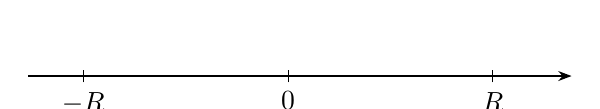
\begin{tikzpicture}[>=Stealth]
\draw[->] (-3.3,0)--(3.6,0);
\foreach \x/\lab in {-2.6/{-R},0/{0},2.6/{R}} {
\draw (\x,-.08)--(\x,.08);
\node[below] at (\x,-.08) {$\lab$};
}
\end{tikzpicture}
\end{center}
\ednote{实谱有界，可取 $R=\|K\|$，使 $\sigma(K)\subset[-R,R]$。
这里 $0$ 是谱点，并不意味着 $0$ 一定是特征值。照片仅给出上述定理的陈述。}

\newpage
\subsection{椭圆算子的形式伴随与弱解}
\source{新板书/02}
沿用前文的散度型算子
\[
Lu=-\sum_{i,j=1}^n(a^{ij}u_{x_i})_{x_j}
   +\sum_{i=1}^nb^iu_{x_i}+cu
\]
及其双线性型 $B[u,v]$。其\textbf{形式伴随算子}为
\[
\boxed{L^*v=-\sum_{i,j=1}^n(a^{ij}v_{x_j})_{x_i}
            -\sum_{i=1}^n(b^iv)_{x_i}+cv.}
\]
当 $b^i$ 可微时，展开一阶项，得到板书中的写法
\[
L^*v=-\sum_{i,j=1}^n(a^{ij}v_{x_j})_{x_i}
     -\sum_{i=1}^nb^iv_{x_i}
     +\left(c-\sum_{i=1}^n b^i_{x_i}\right)v.
\]
\ednote{前文仅假设系数属于 $L^\infty(U)$，此时应使用上面的分布形式或下面的弱形式；
不能默认 $b^i_{x_i}$ 是普通函数。展开式可在 $b^i\in W^{1,\infty}(U)$ 等条件下按函数理解。}

\textbf{伴随方程的弱解。}设 $f\in L^2(U)$。称 $v\in H_0^1(U)$ 为
\[
\begin{cases}
L^*v=f,&\text{于 }U,\\
v=0,&\text{于 }\partial U
\end{cases}
\]
的弱解，若
\[
\boxed{B[u,v]=(f,u)_{L^2(U)},\qquad\forall u\in H_0^1(U).}
\]
这里未知函数在 $B$ 的第二个位置，检验函数在第一个位置。

\textbf{板书中的分部积分核对。}先对光滑函数及零边界检验函数计算，
\[
\begin{aligned}
\int_U(L^*v)u\dd x
&=\int_U\left(\sum_{i,j}a^{ij}v_{x_j}u_{x_i}
 -\sum_i b^iv_{x_i}u
 +\left(c-\sum_i b^i_{x_i}\right)vu\right)\dd x\\
&=\int_U\left(\sum_{i,j}a^{ij}u_{x_i}v_{x_j}
 -\sum_i b^iv_{x_i}u+cuv+\sum_i b^i(uv)_{x_i}\right)\dd x\\
&=\int_U\left(\sum_{i,j}a^{ij}u_{x_i}v_{x_j}
 +\sum_i b^iu_{x_i}v+cuv\right)\dd x
=B[u,v].
\end{aligned}
\]
\ednote{第二步把 $-\int_U b^i_{x_i}uv$ 分部积分；再展开 $(uv)_{x_i}$，
其中的 $b^iuv_{x_i}$ 与前一项相消。这对应照片中的划改。}

\newpage
\subsection{把原方程化为紧算子方程}
\source{新板书/03--05}
取能量估计中的 $\gamma$，必要时增大，使 $\gamma>0$，并令
\[
B_\gamma[u,v]=B[u,v]+\gamma(u,v)_{L^2(U)},\qquad L_\gamma=L+\gamma.
\]
则 $B_\gamma$ 有界且强制：
\[
B_\gamma[u,u]\geq\beta\|u\|_{H_0^1(U)}^2.
\]
由 Lax--Milgram 定理，对任意 $g\in L^2(U)$，存在唯一的 $u\in H_0^1(U)$，使
\[
B_\gamma[u,v]=(g,v)_{L^2(U)},\qquad\forall v\in H_0^1(U).
\]
记此解为 $u=L_\gamma^{-1}g$。

设 $f\in L^2(U)$。原方程的弱形式等价于
\[
\begin{gathered}
B[u,v]=(f,v)_{L^2(U)}\qquad\forall v\in H_0^1(U)\\
\Updownarrow\\
B_\gamma[u,v]=(\gamma u+f,v)_{L^2(U)}\qquad\forall v\in H_0^1(U).
\end{gathered}
\]
从而等价于
\[
u=L_\gamma^{-1}(\gamma u+f).
\]
令
\[
K=\gamma L_\gamma^{-1}:L^2(U)\longrightarrow L^2(U),\qquad
h=L_\gamma^{-1}f.
\]
则得到
\[
\boxed{u-Ku=h.}
\]
更准确地说，
\[
\begin{gathered}
u\in H_0^1(U)\text{ 是 }Lu=f\text{ 的弱解}\\
\Longleftrightarrow\quad
u\in L^2(U)\text{ 满足 }u-Ku=L_\gamma^{-1}f.
\end{gathered}
\]
\ednote{逆向不必预先假定 $u\in H_0^1$：由等式得到
$u=L_\gamma^{-1}(\gamma u+f)\in H_0^1(U)$，再由 $L_\gamma^{-1}$ 的定义恢复弱方程。
这里把 $L_\gamma^{-1}$ 的 $H_0^1$ 值自然看作 $L^2$ 元素。}

特别地，齐次问题对应
\[
Lu=0,\quad u\in H_0^1(U)
\quad\Longleftrightarrow\quad
u-Ku=0,\quad u\in L^2(U).
\]

\newpage
\subsection{紧性与 Fredholm 二择一}
\source{新板书/06、08}
\proofrating{38}{3}{先用能量估计控制逆算子的 $H_0^1$ 范数，再用紧嵌入。}
\textbf{$K$ 的紧性。}由逆算子的定义，
\[
B_\gamma[L_\gamma^{-1}g,v]=(g,v)_{L^2(U)},\qquad
g\in L^2(U),\quad v\in H_0^1(U).
\]
取 $v=L_\gamma^{-1}g$，得到
\[
\begin{aligned}
\beta\|L_\gamma^{-1}g\|_{H_0^1(U)}^2
&\leq B_\gamma[L_\gamma^{-1}g,L_\gamma^{-1}g]\\
&=(g,L_\gamma^{-1}g)_{L^2(U)}\\
&\leq\|g\|_{L^2(U)}\|L_\gamma^{-1}g\|_{H_0^1(U)}.
\end{aligned}
\]
因此
\[
\boxed{\|L_\gamma^{-1}g\|_{H_0^1(U)}
\leq\frac1\beta\|g\|_{L^2(U)}.}
\]
\ednote{该估计先证明 $L_\gamma^{-1}:L^2(U)\to H_0^1(U)$ 有界。
再用有界区域上 $H_0^1(U)\Subset L^2(U)$ 的紧嵌入，便得到
$K=\gamma L_\gamma^{-1}:L^2(U)\to L^2(U)$ 紧；不能仅从有界性直接推出紧性。}

\textbf{Fredholm 二择一。}对上述紧算子 $K$，下列两种情形恰有一种成立：
\begin{enumerate}
\item 对任意 $h\in L^2(U)$，$u-Ku=h$ 在 $L^2(U)$ 中存在唯一解；
\item $u-Ku=0$ 在 $L^2(U)$ 中存在非零解。
\end{enumerate}
记 $K^*$ 为 $K$ 在实 Hilbert 空间 $L^2(U)$ 上的伴随算子，并令
\[
N=\ker(I-K),\qquad N^*=\ker(I-K^*).
\]
则
\[
\boxed{\dim N=\dim N^*<\infty.}
\]
对给定的 $h\in L^2(U)$，有
\[
\boxed{u-Ku=h\text{ 可解}
\quad\Longleftrightarrow\quad
(h,v)_{L^2(U)}=0\quad\forall v\in N^*.}
\]
\ednote{$N^*$ 在这里是伴随齐次方程的解空间记号，不是 $N$ 的对偶空间。}

\newpage
\subsection{辨认紧算子的伴随}
\source{新板书/07、09}
\proofrating{39}{4}{用转置双线性型构造伴随方程的逆，再通过配对验证紧算子的伴随。}
为把 $N^*$ 解释为伴随椭圆方程的解空间，先考虑转置双线性型
\[
B_\gamma^*[v,u]=B_\gamma[u,v].
\]
它同样有界，并且
\[
B_\gamma^*[v,v]=B_\gamma[v,v]\geq\beta\|v\|_{H_0^1(U)}^2.
\]
由 Lax--Milgram 定理，对每个 $g^*\in L^2(U)$，存在唯一的 $v\in H_0^1(U)$，使
\[
B_\gamma[u,v]=(g^*,u)_{L^2(U)},\qquad\forall u\in H_0^1(U).
\]
按照板书记作 $v=L_*^{-1}g^*$，于是
\[
L_*^{-1}:L^2(U)\longrightarrow H_0^1(U)
\]
为有界线性算子，且
\[
B_\gamma[u,L_*^{-1}g^*]=(g^*,u)_{L^2(U)}.
\]
\ednote{本段的 $L_*$ 是移位后的伴随算子，即 $L_*=L^*+\gamma$。
下标星号沿用照片；它与未移位的 $L^*$ 有区别。}

\textbf{证明 $K^*=\gamma L_*^{-1}$。}先令 $S=\gamma L_*^{-1}$，将其看作
$L^2(U)$ 上的有界算子。任取 $g^*,g\in L^2(U)$，由两个逆算子的定义，
\[
\begin{aligned}
(Sg^*,g)_{L^2(U)}
&=B_\gamma[L_\gamma^{-1}g,Sg^*]\\
&=\gamma B_\gamma[L_\gamma^{-1}g,L_*^{-1}g^*]\\
&=\gamma(g^*,L_\gamma^{-1}g)_{L^2(U)}\\
&=(g^*,Kg)_{L^2(U)}.
\end{aligned}
\]
因此由伴随算子的定义，
\[
\boxed{K^*=\gamma L_*^{-1}.}
\]
\ednote{照片用待证的 $K^*$ 直接书写配对。这里先以 $S$ 表示候选算子，
保证 $Sg^*\in H_0^1(U)$，使代入双线性型的每一步均有定义。}

\newpage
\subsection{伴随齐次方程与原方程的可解性}
\source{新板书/07--09}
由 $K^*=\gamma L_*^{-1}$，对 $v\in L^2(U)$，
\[
\begin{gathered}
v-K^*v=0\quad\Longleftrightarrow\quad v=L_*^{-1}(\gamma v)\\
\Updownarrow\\
v\in H_0^1(U),\qquad
B_\gamma[u,v]=(\gamma v,u)_{L^2(U)}\quad\forall u\in H_0^1(U)\\
\Updownarrow\\
v\in H_0^1(U),\qquad B[u,v]=0\quad\forall u\in H_0^1(U).
\end{gathered}
\]
这就是伴随齐次 Dirichlet 问题
\[
L^*v=0\text{ 于 }U,\qquad v=0\text{ 于 }\partial U
\]
的弱解条件。故
\[
\begin{aligned}
N&=\{u\in H_0^1(U):Lu=0\text{（弱意义）}\},\\
N^*&=\{v\in H_0^1(U):L^*v=0\text{（弱意义）}\}.
\end{aligned}
\]
两者均为有限维空间，且维数相同。

\subsection*{回到原方程的正交条件}
\ednote{下面补上从板书中 $h=L_\gamma^{-1}f$ 的正交条件返回原右端项 $f$ 的一步。}
对 $v\in N^*$，有 $L_*^{-1}v=v/\gamma$。因此
\[
\begin{aligned}
(h,v)_{L^2(U)}
&=(L_\gamma^{-1}f,v)_{L^2(U)}\\
&=B_\gamma[L_\gamma^{-1}f,L_*^{-1}v]\\
&=(f,L_*^{-1}v)_{L^2(U)}
=\frac1\gamma(f,v)_{L^2(U)}.
\end{aligned}
\]
结合 Fredholm 二择一，得到
\[
\boxed{\begin{gathered}
Lu=f,\quad u\in H_0^1(U)\text{ 存在弱解}\\
\Longleftrightarrow\quad
(f,v)_{L^2(U)}=0\quad\forall v\in N^*.
\end{gathered}}
\]
\ednote{相应地，若 $N=\{0\}$，则对每个 $f\in L^2(U)$ 都存在唯一弱解；
若 $N\ne\{0\}$，须先满足上面的正交条件，且可解时所有解构成 $u_0+N$。}

\newpage
\fancyhead[R]{\small 2026 年 10 月 28 日}
\begin{center}
  {\Large\bfseries 10 月 28 日：椭圆方程的内部正则性}
\end{center}
\subsection*{前一部分的收尾：齐次特征值方程}
\source{10.28/01 左侧}
板书在前一论证的极限步骤中得到 $u\in H_0^1(U)$，并满足
\[
\int_U\left(\sum_{i,j=1}^n a^{ij}u_{x_i}v_{x_j}
  +\sum_{i=1}^n b^iu_{x_i}v+cuv\right)\dd x
  =\lambda\int_U uv\dd x,
\qquad v\in H_0^1(U).
\]
即 $u$ 是 $Lu=\lambda u$、$u|_{\partial U}=0$ 的弱解。
若 $\lambda$ 不是该 Dirichlet 问题的特征值，则 $u=0$。
\ednote{照片只保留了这一极限论证的末尾，未拍到前面的序列构造；此处保留可见结论。}

\section{椭圆方程的内部正则性}
\subsection{从 Poisson 方程看二阶导数估计}
\source{10.28/01--02}
\proofrating{40}{2}{两次分部积分把拉普拉斯的平方化为二阶导数的平方和。}
先考虑
\[
-\Delta u=f\qquad\text{于 }\R^n.
\]
\ednote{本段先作光滑情形的先验计算，例如取 $u\in C_c^\infty(\R^n)$，
以保证各次分部积分无边界项；这还不是对一般弱解直接求二阶导数。}
由方程与 Young 不等式，
\[
\int_{\R^n}(\Delta u)^2\dd x
=\int_{\R^n}(-\Delta u)f\dd x
\leq\frac12\int_{\R^n}(\Delta u)^2\dd x
  +\frac12\int_{\R^n}f^2\dd x.
\]
另一方面，两次分部积分给出
\[
\begin{aligned}
\int_{\R^n}(\Delta u)^2\dd x
&=\sum_{i,j=1}^n\int_{\R^n}u_{x_ix_i}u_{x_jx_j}\dd x\\
&=-\sum_{i,j=1}^n\int_{\R^n}u_{x_i}u_{x_jx_jx_i}\dd x
=\sum_{i,j=1}^n\int_{\R^n}|u_{x_ix_j}|^2\dd x.
\end{aligned}
\]
故
\[
\boxed{\int_{\R^n}|D^2u|^2\dd x\leq\int_{\R^n}f^2\dd x.}
\]
再对方程求导：$-\Delta u_{x_k}=f_{x_k}$，同理得到
\[
\int_{\R^n}|D^2u_{x_k}|^2\dd x
\leq\int_{\R^n}|f_{x_k}|^2\dd x.
\]
这体现了板书中的阶数关系：$f$ 的一阶导数控制 $u$ 的三阶导数；
一般地，$f$ 的 $m$ 阶导数对应 $u$ 的 $m+2$ 阶导数。

\newpage
\subsection{差商判别的回顾}
\source{10.28/02}
对 $k=1,\ldots,n$，记
\[
D_k^h w(x)=\frac{w(x+he_k)-w(x)}{h},\qquad h\ne0.
\]
设 $V\Subset U$，且 $0<|h|<\tfrac12\operatorname{dist}(V,\partial U)$。
\begin{enumerate}
\item 若 $1\leq p<\infty$、$w\in W^{1,p}(U)$，则
\[
\boxed{\|D_k^h w\|_{L^p(V)}\leq\|w_{x_k}\|_{L^p(U)}.}
\]
\item 若 $1<p<\infty$、$w\in L^p(U)$，且对所有充分小的非零 $h$ 均有
\[
\|D_k^h w\|_{L^p(V)}\leq C_*,
\]
其中 $C_*$ 与 $h$ 无关，则 $w_{x_k}\in L^p(V)$，并有
\[
\boxed{\|w_{x_k}\|_{L^p(V)}\leq C_*.}
\]
\end{enumerate}
\ednote{差商需要用到 $x+he_k$ 处的函数值，故将函数定义在外层区域 $U$；
关键是估计常数不随 $h\to0$ 发散。对每个方向应用第二条即可判定 Sobolev 正则性。}

\subsection{\texorpdfstring{内部 $H^2$ 正则性定理}{内部二阶正则性定理}}
\source{10.28/03；11.2/01 重述}
沿用前文的散度型算子
\[
Lu=-\sum_{i,j=1}^n(a^{ij}u_{x_i})_{x_j}
    +\sum_{i=1}^n b^iu_{x_i}+cu,
\]
并假定主部一致椭圆：存在 $\theta>0$，使
\[
\sum_{i,j=1}^n a^{ij}(x)\xi_i\xi_j\geq\theta|\xi|^2,
\qquad x\in U,\quad\xi\in\R^n.
\]
设
\[
a^{ij}\in C^1(U),\qquad b^i,c\in L^\infty(U),\qquad f\in L^2(U),
\]
且 $u\in H^1(U)$ 是 $Lu=f$ 的弱解，即
\[
B[u,v]=\int_U fv\dd x,\qquad\forall v\in H_0^1(U).
\]
则 $u\in H_{\mathrm{loc}}^2(U)$，且任给 $V\Subset U$，都有
\[
\boxed{\|u\|_{H^2(V)}\leq C\bigl(\|f\|_{L^2(U)}+\|u\|_{L^2(U)}\bigr).}
\]
其中 $C$ 依赖于 $V,U$、椭圆性常数及 $L$ 的系数。
\ednote{这是内部估计，不要求 $u$ 在 $\partial U$ 上为零。
主部系数及其一阶导数只需在证明所用的紧内部邻域上有界。
若系数仅局部有界，弱解等式先对紧支撑测试函数理解即可。}

\newpage
\subsection{截断函数与差商测试函数}
\source{10.28/03--04；11.2/01}
\proofrating{41}{4}{选取二重差商测试函数，利用椭圆性吸收误差，再以局部能量估计消去一阶范数。}
任取 $V\Subset U$，选取中间区域 $W$ 与截断函数 $\zeta$，使
\[
V\Subset W\Subset U,\qquad \zeta\in C_c^\infty(W),\qquad
0\leq\zeta\leq1,\qquad\zeta=1\text{ 于 }V.
\]
\begin{center}
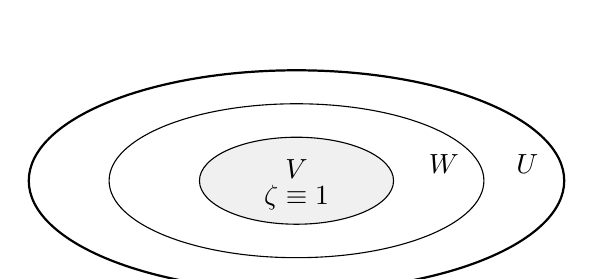
\begin{tikzpicture}[scale=0.85]
\draw[thick] (0,0) ellipse (4.0 and 1.65);
\draw (0,0) ellipse (2.8 and 1.15);
\draw[fill=gray!12] (0,0) ellipse (1.45 and .65);
\node at (3.45,.25){$U$};
\node at (2.2,.25){$W$};
\node at (0,.18){$V$};
\node at (0,-.25){$\zeta\equiv1$};
\end{tikzpicture}
\end{center}
固定方向 $k\in\{1,\ldots,n\}$，取充分小的非零 $h$，令
\[
w=\zeta^2D_k^h u,\qquad
\boxed{v=-D_k^{-h}\bigl(\zeta^2D_k^h u\bigr).}
\]
这里 $h$ 可正可负，并按同一差商定义约定
\[
D_k^{-h}w(x)=\frac{w(x-he_k)-w(x)}{-h}
             =\frac{w(x)-w(x-he_k)}{h}.
\]
\textbf{测试函数的合法性。}由于 $u\in H^1(U)$，对每个固定的充分小的 $h$，
\[
D_k^h u\in H^1(W),\qquad
(D_k^h u)_{x_i}=D_k^h(u_{x_i}).
\]
因此 $w\in H^1(W)$，且其支撑包含在 $\operatorname{supp}\zeta\Subset W$ 内。
将 $w$ 在 $W$ 外延拓为零；再缩小 $|h|$，使其支撑及平移后的支撑均留在 $U$ 内，便有
\[
v=-D_k^{-h}w\in H_0^1(U).
\]
于是可将 $v$ 代入弱解等式：
\[
\int_U\sum_{i,j=1}^n a^{ij}u_{x_i}v_{x_j}\dd x
=\int_U\left(f-\sum_{i=1}^n b^iu_{x_i}-cu\right)v\dd x.
\]
\ednote{此处只用到了固定步长的平移保持 $H^1$，没有预先假设 $u\in H^2$。
接下来需要获得与 $h$ 无关的 $D_k^h Du$ 的 $L^2$ 界，才能由差商判别推出二阶弱导数存在。}

\newpage
\fancyhead[R]{\small 2026 年 11 月 2 日}
\begin{center}
  {\Large\bfseries 11 月 2 日：内部正则性的证明与高阶推广}
\end{center}
\subsection{差商分部积分与主部展开}
\source{11.2/02--04}
继续使用上一页的 $V,W,\zeta,k,h$。记 $q^h(x)=q(x+he_k)$。
在相关支撑及其平移均留在 $U$ 内时，有
\[
\boxed{\int_U pD_k^{-h}q\dd x=-\int_U(D_k^h p)q\dd x,}
\qquad
\boxed{D_k^h(pq)=p^hD_k^h q+(D_k^h p)q.}
\]
\ednote{第一式来自变量平移，第二式来自加减 $p(x+he_k)q(x)$。
在当前证明中，截断函数保证了分部积分不产生区域边缘项。}
为简化记号，令 $\delta=D_k^h$、$u_i=u_{x_i}$、$\zeta_j=\zeta_{x_j}$，并记
\[
I=\int_U\sum_{i,j=1}^n a^{ij}u_i v_{x_j}\dd x,
\qquad v=-D_k^{-h}(\zeta^2\delta u).
\]
差商与弱导数可交换，故
\[
\begin{aligned}
I&=\int_U\sum_{i,j}\delta(a^{ij}u_i)(\zeta^2\delta u)_{x_j}\dd x\\
 &=\int_U\sum_{i,j}
 \bigl((a^{ij})^h\delta u_i+(\delta a^{ij})u_i\bigr)
 \bigl(2\zeta\zeta_j\delta u+\zeta^2\delta u_j\bigr)\dd x\\
 &=\int_U\zeta^2\sum_{i,j}(a^{ij})^h\delta u_i\delta u_j\dd x+R_1+R_2+R_3,
\end{aligned}
\]
其中
\[
\begin{aligned}
R_1&=2\int_U\sum_{i,j}(a^{ij})^h\delta u_i\,\zeta\zeta_j\delta u\dd x,\\
R_2&=2\int_U\sum_{i,j}(\delta a^{ij})u_i\,\zeta\zeta_j\delta u\dd x,\\
R_3&=\int_U\sum_{i,j}(\delta a^{ij})u_i\,\zeta^2\delta u_j\dd x.
\end{aligned}
\]
由系数的 $C^1$ 正则性，$\delta a^{ij}$ 在所用的紧内部区域上一致有界。
将椭圆性应用于 $\xi=\delta Du$，得到
\[
\begin{aligned}
I\geq{}&\theta\int_U\zeta^2|\delta Du|^2\dd x\\
&-C\int_W\bigl(\zeta|\delta Du||\delta u|
 +\zeta|Du||\delta u|+\zeta|Du||\delta Du|\bigr)\dd x.
\end{aligned}
\]
以下常数可依赖截断函数、椭圆性常数及系数，但均与 $h$ 无关。

\newpage
\subsection{吸收误差项并得到一致差商界}
\source{11.2/05--07}
记
\[
A_h=\int_U\zeta^2|\delta Du|^2\dd x,\quad
E=\int_U|Du|^2\dd x,\quad
F=\int_U\bigl(f^2+|Du|^2+u^2\bigr)\dd x.
\]
由差商估计，$\int_W|\delta u|^2\dd x\leq E$。
对含 $\delta Du$ 的两个误差项分别用
$ab\leq\varepsilon a^2+(4\varepsilon)^{-1}b^2$，得到
\[
I\geq(\theta-2\varepsilon)A_h-C_\varepsilon E.
\]
取 $2\varepsilon=\theta/2$，于是
\[
\boxed{I\geq\frac\theta2 A_h-CE.}
\]
另一方面，弱方程右端记为
\[
J=\int_U\left(f-\sum_i b^iu_i-cu\right)v\dd x.
\]
由低阶系数有界，对任意 $\eta>0$，
\[
J\leq |J|\leq\eta\int_Uv^2\dd x+C_\eta F.
\]
将 $\zeta^2\delta u$ 零延拓后应用差商估计，得到
\[
\begin{aligned}
\int_Uv^2\dd x
&=\int_U\bigl|D_k^{-h}(\zeta^2\delta u)\bigr|^2\dd x\\
&\leq\int_U\bigl|D(\zeta^2\delta u)\bigr|^2\dd x\\
&=\int_U\bigl|2\zeta D\zeta\,\delta u+\zeta^2\delta Du\bigr|^2\dd x\\
&\leq 8\int_U\zeta^2|D\zeta|^2|\delta u|^2\dd x
      +2\int_U\zeta^4|\delta Du|^2\dd x
\leq CE+2A_h.
\end{aligned}
\]
利用 $I=J$，并取 $2\eta=\theta/4$，将 $A_h$ 项吸收到左端，得
\[
\frac\theta4 A_h\leq CF.
\]
因 $\zeta=1$ 于 $V$，所以
\[
\boxed{\int_V|D_k^hDu|^2\dd x
\leq C\int_U\bigl(f^2+|Du|^2+u^2\bigr)\dd x.}
\]
右端与 $h$ 无关。对每个 $k$ 应用差商判别，得到 $Du\in H^1(V)$，且
\[
\|u\|_{H^2(V)}\leq C\bigl(\|f\|_{L^2(U)}+\|u\|_{H^1(U)}\bigr).
\]
由于 $V\Subset U$ 任意，已经得到 $u\in H_{\mathrm{loc}}^2(U)$。

\newpage
\subsection{\texorpdfstring{局部能量估计：把右端降到 $L^2$ 范数}{局部能量估计：把右端降到 L² 范数}}
\source{11.2/07--08}
任给 $V\Subset U$，取 $V\Subset W\Subset U$。
把刚才的估计应用于 $V\Subset W$，得到
\[
\|u\|_{H^2(V)}\leq C\bigl(\|f\|_{L^2(W)}
 +\|u\|_{L^2(W)}+\|Du\|_{L^2(W)}\bigr).
\]
为控制最后一项，另取 $\chi\in C_c^\infty(U)$，满足 $0\leq\chi\leq1$、
$\chi=1$ 于 $W$，并将 $v=\chi^2u\in H_0^1(U)$ 代入弱方程。
\ednote{照片此处仍以 $\zeta$ 表示新的截断函数。这里改记为 $\chi$，
以区分前面等于 $1$ 于 $V$ 的截断函数，并展开板书略写的能量估计。}
由 $(\chi^2u)_{x_j}=\chi^2u_j+2\chi\chi_{x_j}u$，得
\[
\begin{aligned}
\int_U\chi^2\sum_{i,j}a^{ij}u_i u_j\dd x
={}&\int_U f\chi^2u\dd x
-2\int_U\sum_{i,j}a^{ij}u_i\chi\chi_{x_j}u\dd x\\
&-\int_U\sum_i b^iu_i\chi^2u\dd x
-\int_U c\chi^2u^2\dd x.
\end{aligned}
\]
利用椭圆性、系数在截断支撑上的界以及 Young 不等式，
\[
\theta\int_U\chi^2|Du|^2\dd x
\leq\frac\theta2\int_U\chi^2|Du|^2\dd x
 +C\int_U(f^2+u^2)\dd x.
\]
吸收后，由 $\chi=1$ 于 $W$，得到
\[
\int_W|Du|^2\dd x\leq\int_U\chi^2|Du|^2\dd x
\leq C\int_U(f^2+u^2)\dd x.
\]
代回上一估计，即得定理中的结论：
\[
\boxed{\|u\|_{H^2(V)}\leq C\bigl(\|f\|_{L^2(U)}+\|u\|_{L^2(U)}\bigr).}
\]

\subsection*{板书中的零边界 Poisson 方程示例}
若 $-\Delta u=f$ 于 $U$、$u\in H_0^1(U)$，以 $u$ 为测试函数，得到
\[
\int_U|Du|^2\dd x=\int_U fu\dd x
\leq\varepsilon\int_Uu^2\dd x+\frac1{4\varepsilon}\int_Uf^2\dd x
\leq\varepsilon C_P\int_U|Du|^2\dd x
 +\frac1{4\varepsilon}\int_Uf^2\dd x.
\]
这里使用 Poincar\'e 不等式。取 $\varepsilon C_P<1$，即可控制 $\|Du\|_{L^2(U)}$。
\ednote{这一示例依赖零边界条件；一般内部正则性证明使用上面的截断测试函数，保留 $\|u\|_{L^2(U)}$ 项。}

\newpage
\subsection{高阶内部正则性}
\source{11.2/09--10}
\textbf{定理。}设 $m\geq0$ 为整数，主部仍一致椭圆，并且
\[
a^{ij}\in C^{m+1}(U),\qquad b^i,c\in C^m(U),\qquad f\in H^m(U).
\]
若 $u\in H^1(U)$ 是 $Lu=f$ 于 $U$ 的弱解，则
\[
u\in H_{\mathrm{loc}}^{m+2}(U),
\]
且对任意 $V\Subset U$，
\[
\boxed{\|u\|_{H^{m+2}(V)}
\leq C\bigl(\|f\|_{H^m(U)}+\|u\|_{L^2(U)}\bigr).}
\]
其中 $C$ 依赖于 $m,V,U$、椭圆性常数及系数的相应局部导数界。

\proofrating{42}{4}{对方程作弱微分，将系数导数产生的项移入右端，再对高阶导数应用内部 $H^2$ 定理。}
\textbf{归纳起点。}$m=0$ 即刚证明的内部 $H^2$ 正则性。

\textbf{归纳步骤。}假设 $m$ 阶结论成立。现设
\[
a^{ij}\in C^{m+2}(U),\qquad b^i,c\in C^{m+1}(U),\qquad f\in H^{m+1}(U),
\]
要证明 $u\in H_{\mathrm{loc}}^{m+3}(U)$。
任取 $V\Subset W\Subset U$，由归纳假设，
\[
u\in H^{m+2}(W),\qquad
\|u\|_{H^{m+2}(W)}
\leq C\bigl(\|f\|_{H^m(U)}+\|u\|_{L^2(U)}\bigr).
\]
固定多重指标 $\alpha$，满足 $|\alpha|=m+1$，令
\[
\widetilde u=D^\alpha u\in H^1(W).
\]
对任意 $\widetilde v\in C_c^\infty(W)$，取
$v=(-1)^{|\alpha|}D^\alpha\widetilde v\in H_0^1(U)$。
将其代入原弱方程，并把 $D^\alpha$ 从测试函数上移开，得到
\[
\begin{aligned}
\int_W\Bigl(&\sum_{i,j}D^\alpha(a^{ij}u_i)\widetilde v_{x_j}
 +\sum_iD^\alpha(b^iu_i)\widetilde v
 +D^\alpha(cu)\widetilde v\Bigr)\dd x
=\int_W D^\alpha f\,\widetilde v\dd x.
\end{aligned}
\]
接下来用多重指标的 Leibniz 公式展开，分离出系数未被求导的项，
使左端恢复为 $B[\widetilde u,\widetilde v]$。

\newpage
\subsection{高阶导数满足的方程与归纳闭合}
\source{11.2/10--11}
约定 $\beta\leq\alpha$ 表示逐分量不等式，
$\binom\alpha\beta=\prod_{\ell=1}^n\binom{\alpha_\ell}{\beta_\ell}$。
例如
\[
D^\alpha(a^{ij}u_i)
=a^{ij}\widetilde u_{x_i}
 +\sum_{\substack{\beta\leq\alpha\\\beta\ne\alpha}}
 \binom\alpha\beta(D^{\alpha-\beta}a^{ij})D^\beta u_i.
\]
将这些余项移到右端，并对主部余项再作一次分部积分，得到
\[
B[\widetilde u,\widetilde v]=\int_W\widetilde f\,\widetilde v\dd x,
\qquad\widetilde v\in C_c^\infty(W),
\]
其中
\[
\boxed{\begin{aligned}
\widetilde f={}&D^\alpha f
 +\sum_{i,j=1}^n\sum_{\substack{\beta\leq\alpha\\\beta\ne\alpha}}
 \binom\alpha\beta
 \bigl((D^{\alpha-\beta}a^{ij})D^\beta u_i\bigr)_{x_j}\\
&-\sum_{i=1}^n\sum_{\substack{\beta\leq\alpha\\\beta\ne\alpha}}
 \binom\alpha\beta(D^{\alpha-\beta}b^i)D^\beta u_i\\
&-\sum_{\substack{\beta\leq\alpha\\\beta\ne\alpha}}
 \binom\alpha\beta(D^{\alpha-\beta}c)D^\beta u.
\end{aligned}}
\]
\textbf{检查右端的正则性。}由于 $\beta\ne\alpha$，有 $|\beta|\leq m$。
主部余项展开为
\[
\bigl((D^{\alpha-\beta}a^{ij})D^\beta u_i\bigr)_{x_j}
=(D^{\alpha-\beta+e_j}a^{ij})D^\beta u_i
 +(D^{\alpha-\beta}a^{ij})D^{\beta+e_j}u_i.
\]
其中对 $u$ 最多求 $m+2$ 阶导数，对 $a^{ij}$ 最多求 $m+2$ 阶导数，
均由归纳假设与当前系数条件控制。低阶余项同理。因此
\[
\begin{aligned}
\|\widetilde f\|_{L^2(W)}
&\leq C\bigl(\|f\|_{H^{m+1}(W)}+\|u\|_{H^{m+2}(W)}\bigr)\\
&\leq C\bigl(\|f\|_{H^{m+1}(U)}+\|u\|_{L^2(U)}\bigr).
\end{aligned}
\]
于是 $\widetilde u\in H^1(W)$ 是 $L\widetilde u=\widetilde f$ 的弱解。
对它应用内部 $H^2$ 定理，得到
\[
\begin{aligned}
\|D^\alpha u\|_{H^2(V)}
&\leq C\bigl(\|\widetilde f\|_{L^2(W)}+\|D^\alpha u\|_{L^2(W)}\bigr)\\
&\leq C\bigl(\|f\|_{H^{m+1}(U)}+\|u\|_{L^2(U)}\bigr).
\end{aligned}
\]
对所有 $|\alpha|=m+1$ 求和，并结合已有的低阶估计，得
\[
\boxed{\|u\|_{H^{m+3}(V)}
\leq C\bigl(\|f\|_{H^{m+1}(U)}+\|u\|_{L^2(U)}\bigr).}
\]
故归纳步骤成立，高阶内部正则性定理得证。

\newpage
\fancyhead[R]{\small 2026 年 11 月 9 日}
\begin{center}
  {\Large\bfseries 11 月 9 日：边界正则性与最大值原理}
\end{center}
\section{椭圆方程的边界正则性}
\subsection{\texorpdfstring{边界 $H^2$ 估计}{边界二阶估计}}
\source{11.9/01（归纳起点）}
\ednote{照片从高阶边界正则性的归纳步骤开始。下文先补记板书用到的 $m=0$ 结论及其证明。}
\textbf{定理。}设 $U$ 为有界开集，$\partial U$ 为 $C^2$，
$a^{ij}\in C^1(\Ub)$，$b^i,c\in L^\infty(U)$，主部一致椭圆。
若 $f\in L^2(U)$，且 $u\in H_0^1(U)$ 是 $Lu=f$ 的弱解，则
\[
\boxed{u\in H^2(U),\qquad
\|u\|_{H^2(U)}\le C\bigl(\|f\|_{L^2(U)}+\|u\|_{L^2(U)}\bigr).}
\]

\proofrating{43}{4}{展平边界后沿切向使用差商，借助方程控制剩下的纯法向二阶导数。}
\textbf{展平边界。}在每个边界点附近，将区域变为半球 $B_s^+=B(0,s)\cap\{x_n>0\}$，
真实边界变为平面部分 $\Gamma_s=B(0,s)\cap\{x_n=0\}$。
弱方程仍为散度型，变换后的主部仍一致椭圆，且 $u$ 在 $\Gamma_s$ 上的迹为零。
以下沿用 $u,a^{ij},b^i,c,f$ 表示变换后的函数。
局部测试函数在 $\Gamma_s$ 上零迹，且在球面部分附近为零。

\textbf{切向差商。}任取 $0<t<r<s$，再选 $t<\rho<r$。
取截断函数 $\eta\in C_c^\infty(B(0,\rho))$，
使 $\eta=1$ 于 $B(0,t)$ 且 $0\le\eta\le1$。对 $k<n$，
在半球上的弱方程中取
\[
v=-D_k^{-h}(\eta^2D_k^hu).
\]
沿 $e_k$ 的平移保持平面边界，故 $v$ 的平面迹为零。取 $|h|$ 足够小，
差商分部积分后的主部由
\[
D_k^h(a^{ij}u_i)
=a^{ij}(x+he_k)D_k^hu_i+(D_k^ha^{ij})u_i
\]
展开。椭圆项控制 $\|\eta D_k^h Du\|_{L^2}^2$。截断函数导数项、系数差商项用
$\|D_k^h u\|_{L^2(B_\rho^+)}\le\|Du\|_{L^2(B_r^+)}$ 和 Young 不等式估计。
将低阶项移到右端并使用
\[
\|v\|_{L^2(B_r^+)}\le
C\bigl(\|\eta D_k^h Du\|_{L^2(B_r^+)}+\|Du\|_{L^2(B_r^+)}\bigr),
\]
即可吸收含 $\eta D_k^h Du$ 的误差，得到与 $h$ 无关的估计
\[
\|D_k^h Du\|_{L^2(B_t^+)}
\le C\bigl(\|f\|_{L^2(B_r^+)}+\|u\|_{H^1(B_r^+)}\bigr).
\]
差商判别给出 $u_{x_ix_k}\in L^2(B_t^+)$，其中 $i$ 任意、$k<n$。

\newpage
\subsection{纯法向二阶导数与整体估计}
\source{11.9/01（归纳起点）}
在分布意义下展开 $Lu=f$，得到
\[
\begin{aligned}
a^{nn}u_{x_nx_n}
={}&-f-\sum_{i,j=1}^n a^{ij}_{x_j}u_{x_i}
 -\sum_{(i,j)\ne(n,n)}a^{ij}u_{x_ix_j}\\
&+\sum_{i=1}^n b^iu_{x_i}+cu.
\end{aligned}
\]
右端的二阶导数均含至少一次切向微分。由 $a^{nn}\ge\theta>0$，
方程给出 $u_{x_nx_n}\in L^2(B_t^+)$，并得到相同形式的 $L^2$ 估计。
这里可以先由内部正则性在 $B_t^+$ 的每个内部点附近使用该恒等式，
再由右端的估计获得整个 $B_t^+$ 上的可积性。

取稍大的半球估计一阶项。以 $\zeta^2u$ 为测试函数，其中 $\zeta$ 是支撑于
较大球内的截断函数且在较小球上等于 $1$，由零迹、椭圆性和 Young 不等式得
\[
\|Du\|_{L^2(B_r^+)}
\le C\bigl(\|f\|_{L^2(B_s^+)}+\|u\|_{L^2(B_s^+)}\bigr).
\]
在切向差商及法向恢复的估计中用中间半球的这一界，即可得到局部形式
\[
\boxed{\|u\|_{H^2(B_t^+)}
\le C\bigl(\|f\|_{L^2(B_s^+)}+\|u\|_{L^2(B_s^+)}\bigr).}
\]
将半球上的估计转回原坐标，有限覆盖 $\partial U$，再与内部估计合并，即得整体结论。

\subsection{高阶边界正则性}
\source{11.9/01--03}
\textbf{定理。}设 $m\ge0$ 为整数，$U$ 有界，$\partial U$ 为 $C^{m+2}$，
主部一致椭圆，并设
\[
a^{ij}\in C^{m+1}(\Ub),\qquad
b^i,c\in C^m(\Ub),\qquad f\in H^m(U).
\]
若 $u\in H_0^1(U)$ 是 $Lu=f$ 的弱解，则
\[
\boxed{u\in H^{m+2}(U),\qquad
\|u\|_{H^{m+2}(U)}
\le C\bigl(\|f\|_{H^m(U)}+\|u\|_{L^2(U)}\bigr).}
\]
常数 $C$ 依赖于 $m,U$、椭圆性常数及系数的相应范数。

\newpage
\subsection{对切向导数应用边界二阶估计}
\source{11.9/01--03}
\proofrating{44}{4}{先按总阶数归纳，再按同一总阶数下的法向微分次数归纳。}
\textbf{按总阶数归纳。}展平边界后证明对应的局部估计，再用有限覆盖和内部正则性得到整体估计。
取 $0<t<r<s$，记
\[
\widetilde V=B_t^+,\qquad
\widetilde W=B_r^+,\qquad
\widetilde U=B_s^+.
\]
\begin{center}
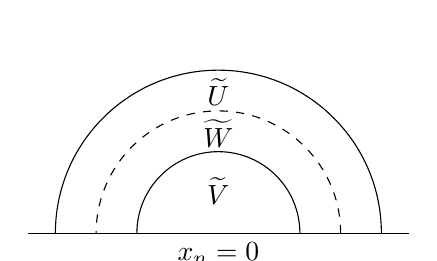
\begin{tikzpicture}[scale=1.15]
  \draw (-2.1,0) -- (2.1,0);
  \draw (1.8,0) arc[start angle=0,end angle=180,radius=1.8];
  \draw[dashed] (1.35,0) arc[start angle=0,end angle=180,radius=1.35];
  \draw (0.9,0) arc[start angle=0,end angle=180,radius=0.9];
  \node at (0,0.47) {$\widetilde V$};
  \node at (0,1.1) {$\widetilde W$};
  \node at (0,1.56) {$\widetilde U$};
  \node[anchor=north] at (0,0) {$x_n=0$};
\end{tikzpicture}
\end{center}
$m=0$ 是边界 $H^2$ 估计。假设已证 $m$ 阶结论，现取
$a^{ij}\in C^{m+2}$、$b^i,c\in C^{m+1}$、$f\in H^{m+1}$、$\partial U$ 为 $C^{m+3}$。
展平后由归纳假设有
\[
\|u\|_{H^{m+2}(\widetilde W)}
\le C\bigl(\|f\|_{H^m(\widetilde U)}+\|u\|_{L^2(\widetilde U)}\bigr).
\]
内部正则性同时给出 $u\in H_{\mathrm{loc}}^{m+3}(U)$。

\textbf{至多两次法向微分。}取 $|\alpha|=m+1$ 且 $\alpha_n=0$，令
$\widetilde u=D^\alpha u$。由上式 $\widetilde u\in H^1(\widetilde W)$。
由于 $\alpha$ 只含切向微分，取迹与切向微分可交换，所以 $\widetilde u$ 在
$\Gamma_r$ 上的迹为零。和内部正则性的证明一样，对弱方程作切向微分得到
$L\widetilde u=\widetilde f$。切向微分保持平面上的零迹测试条件。
将主部余项写成散度移到右端，分部积分时边界项因测试函数零迹而消失。从而
\[
\begin{aligned}
\widetilde f={}&D^\alpha f
+\sum_{i,j=1}^n\sum_{\substack{\beta\le\alpha\\\beta\ne\alpha}}
\binom\alpha\beta\bigl((D^{\alpha-\beta}a^{ij})D^\beta u_{x_i}\bigr)_{x_j}\\
&-\sum_{i=1}^n\sum_{\substack{\beta\le\alpha\\\beta\ne\alpha}}
\binom\alpha\beta(D^{\alpha-\beta}b^i)D^\beta u_{x_i}\\
&-\sum_{\substack{\beta\le\alpha\\\beta\ne\alpha}}
\binom\alpha\beta(D^{\alpha-\beta}c)D^\beta u.
\end{aligned}
\]

\newpage
\subsection{按法向微分次数恢复高阶导数}
\source{11.9/02--05}
由于 $|\beta|\le m$，右端至多含 $u$ 的 $m+2$ 阶导数。结合归纳假设，
有 $\widetilde f\in L^2(\widetilde W)$，且
\[
\|\widetilde f\|_{L^2(\widetilde W)}
\le C\bigl(\|f\|_{H^{m+1}(\widetilde U)}+\|u\|_{L^2(\widetilde U)}\bigr).
\]
对 $\widetilde u$ 应用局部边界 $H^2$ 估计，
\[
\begin{aligned}
\|\widetilde u\|_{H^2(\widetilde V)}
&\le C\bigl(\|\widetilde f\|_{L^2(\widetilde W)}
            +\|\widetilde u\|_{L^2(\widetilde W)}\bigr)\\
&\le C\bigl(\|f\|_{H^{m+1}(\widetilde U)}+\|u\|_{L^2(\widetilde U)}\bigr).
\end{aligned}
\]
因此对 $|\beta|=m+3$ 且 $\beta_n\le2$，$D^\beta u$ 在 $\widetilde V$ 上已有上述 $L^2$ 界。

\textbf{增加法向微分次数。}设该界已对 $|\beta|=m+3$、$\beta_n\le j$ 成立，
其中 $2\le j\le m+2$。取 $|\eta|=m+3$、$\eta_n=j+1$，
写成 $\eta=\gamma+2e_n$，于是 $|\gamma|=m+1$、$\gamma_n=j-1$。
由内部正则性可在内部对 $Lu=f$ 作 $D^\gamma$ 微分，
分离出纯法向项后有
\[
\begin{aligned}
a^{nn}D^\eta u={}&-D^\gamma f
-\sum_{i,j=1}^n D^\gamma(a^{ij}_{x_j}u_{x_i})
-\sum_{(i,j)\ne(n,n)}D^\gamma(a^{ij}u_{x_ix_j})\\
&-\sum_{\substack{\sigma\le\gamma\\\sigma\ne\gamma}}
\binom\gamma\sigma(D^{\gamma-\sigma}a^{nn})D^\sigma u_{x_nx_n}\\
&+\sum_{i=1}^nD^\gamma(b^iu_{x_i})+D^\gamma(cu).
\end{aligned}
\]
其中总阶数为 $m+3$ 的导数只能来自非 $(n,n)$ 的二阶项，
故至多含 $(j-1)+1=j$ 次法向微分，已有 $L^2$ 界。
其余项最多用到 $u$ 的 $m+2$ 阶导数，由总阶数的归纳假设控制。
由 $a^{nn}\ge\theta$，得到
\[
\|D^\eta u\|_{L^2(\widetilde V)}
\le C\bigl(\|f\|_{H^{m+1}(\widetilde U)}+\|u\|_{L^2(\widetilde U)}\bigr).
\]
递推至 $j+1=m+3$，结合低阶导数的估计，得到 $\widetilde V$ 上的
$H^{m+3}$ 估计，完成总阶数的归纳。
\ednote{照片 03 的法向次数归纳上界写作 $n-1$。按所估导数的总阶数 $m+3$，归纳参数应取至 $m+2$，从而覆盖纯法向的 $m+3$ 阶导数。}

\newpage
\subsection{光滑数据与直到边界的光滑性}
\source{11.9/06}
\textbf{推论。}若 $a^{ij},b^i,c,f\in C^\infty(\Ub)$，$\partial U$ 为 $C^\infty$，
且 $u\in H_0^1(U)$ 是齐次 Dirichlet 问题的弱解，则 $u\in C^\infty(\Ub)$。
事实上，高阶边界正则性给出任意整数阶的 $H^k(U)$ 正则性，
再对任意整数 $\ell\ge0$ 选 $k>\ell+n/2$，由 Sobolev 嵌入得到
$u\in C^\ell(\Ub)$。

\section{椭圆方程的最大值原理}
\subsection{零阶系数为零时的弱最大值原理}
\source{11.9/06--09、11--12}
此处采用非散度型写法
\[
Lu=-\sum_{i,j=1}^na^{ij}u_{x_ix_j}
   +\sum_{i=1}^nb^iu_{x_i}+cu,
\]
其中 $U$ 是有界开集，$a^{ij},b^i,c\in C(\Ub)$，$a^{ij}=a^{ji}$，
且主部满足一致椭圆性，椭圆性常数记为 $\theta>0$。

\textbf{定理。}设 $u\in C^2(U)\cap C(\Ub)$，且 $c=0$ 于 $U$。
若 $Lu\le0$ 于 $U$，则 $\max_{\Ub}u=\max_{\partial U}u$。
若 $Lu\ge0$ 于 $U$，则 $\min_{\Ub}u=\min_{\partial U}u$。
在此符号约定下，满足 $Lu\le0$ 的 $u$ 称为 $Lu=0$ 的下解。

\proofrating{45}{3}{先排除严格下解的内部最大值，再用指数函数把非严格不等式变严格。}
\textbf{严格情形。}设 $Lu<0$。若 $u$ 在 $x^0\in U$ 达到最大值，
则 $Du(x^0)=0$，且 $D^2u(x^0)$ 半负定。
取正交矩阵 $Q=(q_{ij})$，使
\[
Q(a^{ij}(x^0))Q^\mathsf{T}=\operatorname{diag}(d_1,\ldots,d_n),
\qquad d_k>0.
\]
令 $y=x^0+Q(x-x^0)$、$v(y)=u(x)$，则
$u_{x_ix_j}=\sum_{k,\ell}v_{y_ky_\ell}q_{ki}q_{\ell j}$，从而
\[
\sum_{i,j=1}^n a^{ij}(x^0)u_{x_ix_j}(x^0)
=\sum_{k=1}^n d_kv_{y_ky_k}(x^0)\le0.
\]
于是 $Lu(x^0)\ge0$，矛盾。因此 $u$ 的最大值只能在边界上达到。

\newpage
\subsection{指数扰动与非负零阶系数}
\source{11.9/09--12}
\textbf{非严格情形。}设 $Lu\le0$，令
$u^\varepsilon(x)=u(x)+\varepsilon e^{\lambda x_1}$，其中 $\varepsilon>0$。
由于 $a^{11}\ge\theta$，
\[
\begin{aligned}
Lu^\varepsilon
&\le\varepsilon L(e^{\lambda x_1})
=\varepsilon e^{\lambda x_1}(-a^{11}\lambda^2+b^1\lambda)\\
&\le \varepsilon e^{\lambda x_1}
\bigl(-\theta\lambda^2+\lambda\|b^1\|_{L^\infty(U)}\bigr)<0
\end{aligned}
\]
只要 $\lambda$ 充分大。故 $\max_{\Ub}u^\varepsilon=\max_{\partial U}u^\varepsilon$。
由 $U$ 有界，$u^\varepsilon\to u$ 在 $\Ub$ 上一致成立，令 $\varepsilon\downarrow0$
即得最大值结论。对 $-u$ 应用最大值结论即得最小值结论。

\textbf{定理。}设 $u\in C^2(U)\cap C(\Ub)$，且 $c\ge0$ 于 $U$。
\begin{itemize}
\item 若 $Lu\le0$ 于 $U$ 且 $\max_{\Ub}u\ge0$，则
$\max_{\Ub}u=\max_{\partial U}u$。
\item 若 $Lu\ge0$ 于 $U$ 且 $\min_{\Ub}u\le0$，则
$\min_{\Ub}u=\min_{\partial U}u$。
\end{itemize}
因此，$Lu\le0$ 时有 $\max_{\Ub}u^+=\max_{\partial U}u^+$，
$Lu\ge0$ 时有 $\max_{\Ub}u^-=\max_{\partial U}u^-$，
其中 $u^+=\max\{u,0\}$、$u^-=\max\{-u,0\}$。

\proofrating{46}{3}{非负的内部最大值处，零阶项也非负，同一指数扰动仍可使用。}
若严格下解在 $x^0\in U$ 达到非负最大值，则 $c(x^0)u(x^0)\ge0$，
与主部和一阶项的符号合起来给出 $Lu(x^0)\ge0$，矛盾。
一般情形仍取 $u^\varepsilon=u+\varepsilon e^{\lambda x_1}$，
此时
\[
L(e^{\lambda x_1})\le e^{\lambda x_1}
\bigl(-\theta\lambda^2+\lambda\|b^1\|_{L^\infty(U)}
+\|c\|_{L^\infty(U)}\bigr)<0
\]
对充分大的固定 $\lambda$ 成立。由于 $\max_{\Ub}u^\varepsilon>0$，
严格情形适用。令 $\varepsilon\downarrow0$ 即得第一条，对 $-u$ 应用第一条得到第二条。

\newpage
\subsection{Hopf 边界点引理}
\source{11.9/11--12；11.11/01 重述}
\textbf{引理。}设 $B=B(z,R)$ 为开球，$u\in C^2(B)\cap C^1(\overline B)$，
$c\ge0$ 且 $Lu\le0$ 于 $B$。若存在 $x^0\in\partial B$ 满足
\[
u(x^0)\ge0,\qquad u(x)<u(x^0)\quad (x\in B),
\]
则沿球面的外单位法向 $\nu=(x^0-z)/R$，
\[
\boxed{\frac{\partial u}{\partial\nu}(x^0)>0.}
\]
\begin{center}
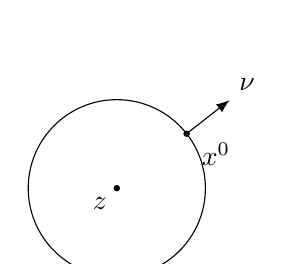
\begin{tikzpicture}[scale=0.9,>=Latex]
  \draw (0,0) circle[radius=1.25];
  \fill (0,0) circle[radius=1.3pt] node[below left] {$z$};
  \fill (38:1.25) circle[radius=1.3pt] node[below right,xshift=2pt] {$x^0$};
  \draw[->] (38:1.25) -- (38:2.02) node[above right] {$\nu$};
\end{tikzpicture}
\end{center}

\subsection{一维辅助比较}
\source{11.9/12}
\textbf{引理（第一部分）。}设 $x^0>0$，$f\in C^1([0,x^0])$，$f<0$ 于 $[0,x^0)$，
且 $f(x^0)=0$、$f'(x^0)>0$。若 $g\in C^1([0,x^0])$，
$g<0$ 于 $[0,x^0)$ 且 $g(x^0)=0$，则充分小的 $\varepsilon>0$ 满足
\[
\varepsilon g(x)\ge f(x),\qquad x\in[0,x^0].
\]
\begin{center}
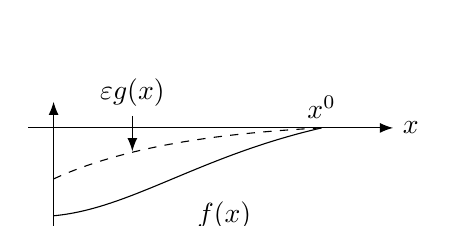
\begin{tikzpicture}[x=1.15cm,y=0.9cm,>=Latex]
  \draw[->] (-0.28,0) -- (3.75,0) node[right] {$x$};
  \draw[->] (0,-1.53) -- (0,0.37);
  \draw (0,-1.24) .. controls (0.85,-1.14) and (1.6,-0.4) .. (2.96,0)
    node[above] {$x^0$};
  \draw[dashed] (0,-0.72) .. controls (0.75,-0.28) and (1.75,-0.08) .. (2.96,0);
  \node[above] at (0.87,0.17) {$\varepsilon g(x)$};
  \draw[->,thin] (0.87,0.17) -- (0.87,-0.33);
  \node at (1.48,-0.91) [below right] {$f(x)$};
\end{tikzpicture}
\end{center}
\proofrating{47}{2}{把比较化为商的上界，并利用端点处非零的一阶导数。}
在 $[0,x^0)$ 上，除以 $f(x)<0$ 后，所求不等式等价于
$g(x)/f(x)\le 1/\varepsilon$。
\ednote{板书写到商的上界。可由端点处的一阶展开补全这一步。}
由于 $f'(x^0)>0$，
\[
\lim_{x\uparrow x^0}\frac{g(x)}{f(x)}=\frac{g'(x^0)}{f'(x^0)}.
\]
故该商可连续延拓到闭区间，具有有限上界。取 $\varepsilon$ 使 $1/\varepsilon$
大于该上界，端点处则两边都为零。

\newpage
\fancyhead[R]{\small 2026 年 11 月 11 日}
\begin{center}
  {\Large\bfseries 11 月 11 日：强最大值原理与椭圆特征值}
\end{center}

\subsection*{一维比较的续证}
\source{11.11/01--02}
仍设 $f\in C^1([0,x^0])$，$f<0$ 于 $[0,x^0)$，且 $f(x^0)=0$。

\textbf{第二条。}若存在 $g\in C^1([0,x^0])$ 和 $\varepsilon>0$，使
\[
g<0\ \text{于 }[0,x^0),\qquad
g(x^0)=0,\qquad g'(x^0)>0,\qquad
f\leq\varepsilon g\ \text{于 }[0,x^0],
\]
则 $f'(x^0)>0$。

\textbf{证明。}令 $H=f-\varepsilon g$。由 $H\leq0$ 及 $H(x^0)=0$，
在右端点取左导数，得 $H'(x^0)\geq0$。因此
\[
f'(x^0)\geq\varepsilon g'(x^0)>0.
\]

\subsection*{Hopf 边界点引理的证明}
\source{11.11/02--03；04 左侧为续写}
\proofrating{48}{4}{在内切球的环带上构造指数障碍函数，用弱最大值原理比较，再沿外法线取导数。}
平移球心后设 $B=B(0,R)$，记
\[
B^*=B(0,R)\setminus\overline{B(0,R/2)},\qquad
v(x)=e^{-\lambda |x|^2}-e^{-\lambda R^2},
\qquad w(x)=u(x)-u(x^0)+\varepsilon v(x).
\]
其中 $\lambda>0$ 取充分大，再取充分小的 $\varepsilon>0$。
外球面上 $v=0$，环带内 $0<v<1$。

\begin{center}
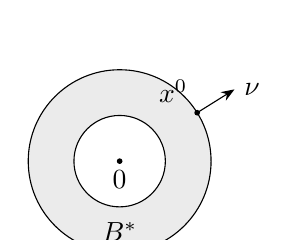
\begin{tikzpicture}[scale=0.86,>=Stealth]
  \fill[gray!16,even odd rule] (0,0) circle (1.35) (0,0) circle (0.675);
  \draw (0,0) circle (1.35);
  \draw (0,0) circle (0.675);
  \fill (0,0) circle (1.2pt) node[below] {$0$};
  \fill (32:1.35) circle (1.2pt) node[above left] {$x^0$};
  \draw[->] (32:1.35) -- (32:2.0) node[right] {$\nu$};
  \node at (0,-1.04) {$B^*$};
\end{tikzpicture}
\end{center}

记 $A=(a^{ij})$、$b=(b^1,\ldots,b^n)$。用上次课的非散度型算子
$Lv=-\sum_{i,j}a^{ij}v_{x_ix_j}+\sum_i b^i v_{x_i}+cv$，先计算
\[
v_{x_i}=-2\lambda x_i e^{-\lambda|x|^2},\qquad
v_{x_ix_j}=(4\lambda^2x_ix_j-2\lambda\delta_{ij})e^{-\lambda|x|^2}.
\]

\newpage
\subsection*{Hopf 引理的证明（续）}
\source{11.11/03--04}
利用 $c\geq0$、一致椭圆性和 $R/2<|x|<R$，有
\[
\begin{aligned}
e^{\lambda |x|^2}Lv
&=2\lambda\operatorname{tr}A
  -4\lambda^2\sum_{i,j}a^{ij}x_ix_j
  -2\lambda b\cdot x+c\bigl(1-e^{-\lambda(R^2-|x|^2)}\bigr)\\
&\leq 2\lambda\operatorname{tr}A-4\lambda^2\theta|x|^2
  -2\lambda b\cdot x+c\\
&\leq 2\lambda\|\operatorname{tr}A\|_{L^\infty(B)}
  -\lambda^2\theta R^2
  +2\lambda R\|b\|_{L^\infty(B)}+\|c\|_{L^\infty(B)}.
\end{aligned}
\]
\ednote{板书在合并主部各项时略去了 $\operatorname{tr}A$ 前的因子 $2\lambda$，这里按二阶导数的计算补齐。}
取 $\lambda$ 充分大，得 $Lv\leq0$ 于 $B^*$。因为 $u(x^0)\geq0$，
\[
Lw=Lu-c(x)u(x^0)+\varepsilon Lv\leq0\qquad\text{于 }B^*.
\]
由 $u(x)<u(x^0)$ 于 $B$ 及 $u$ 的连续性，$w\leq0$ 于外球面。
在内球面上，
\[
\left.w\right|_{|x|=R/2}
\leq\max_{|y|=R/2}u(y)-u(x^0)+\varepsilon .
\]
取 $0<\varepsilon<u(x^0)-\max_{|y|=R/2}u(y)$，得 $w\leq0$ 于内球面。
在 $B^*$ 上应用弱最大值原理，得到
\[
w(x)\leq0=w(x^0).
\]
沿由球内指向 $x^0$ 的外法向取差商，知
$\partial_\nu w(x^0)\geq0$。另一方面，
\[
\partial_\nu v(x^0)
=Dv(x^0)\cdot\frac{x^0}{R}
=-2\lambda R e^{-\lambda R^2}<0.
\]
于是
\[
\boxed{\partial_\nu u(x^0)
=\partial_\nu w(x^0)-\varepsilon\partial_\nu v(x^0)>0.}
\]

\newpage
\subsection{强最大值原理}
\source{11.11/05；06 左侧}
\textbf{定理。}设 $U\subset\R^n$ 为有界连通开集，
$u\in C^2(U)\cap C(\Ub)$，$c\geq0$，且 $Lu\leq0$ 于 $U$。
若 $u$ 非常数，则 $u$ 的非负最大值只能在 $\partial U$ 上取到。
换言之，若存在 $x^1\in U$ 使 $u(x^1)=\max_{\Ub}u\geq0$，
则 $u$ 在 $U$ 上为常数。

\proofrating{49}{4}{沿路径找到离最大值集合足够近的非最大值点，以它为球心构造内切球并应用 Hopf 引理。}
\textbf{证明。}反设存在 $x^1,x^2\in U$，使
\[
u(x^1)=\max_{\Ub}u=:M\geq0,\qquad u(x^2)<M.
\]
由连通性，可在 $U$ 内以路径 $\Gamma$ 连接 $x^1$ 与 $x^2$。取
\[
0<\delta<\frac14\operatorname{dist}(\Gamma,\partial U),
\]
沿路径选取 $y^1=x^1,y^2,\ldots,y^N=x^2$，使相邻点满足
$|y^{i+1}-y^i|<\delta$，并作开球 $B(y^i,\delta)$。

\begin{center}
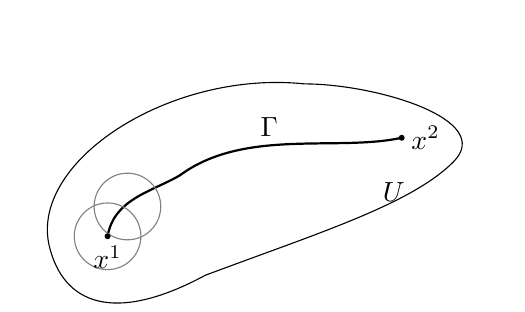
\begin{tikzpicture}[scale=0.9]
  \draw (-0.6,0.2) .. controls (-0.9,1.4) and (1.1,2.7) .. (3.0,2.5)
       .. controls (4.0,2.5) and (5.7,2.0) .. (5.1,1.4)
       .. controls (4.5,0.8) and (3.2,0.4) .. (1.6,-0.2)
       .. controls (0.3,-0.9) and (-0.4,-0.6) .. (-0.6,0.2);
  \draw[thick] (0.22,0.35) .. controls (0.31,0.88) and (0.85,0.98) .. (1.24,1.21)
       .. controls (2.15,1.88) and (3.46,1.54) .. (4.37,1.74);
  \draw[gray] (0.22,0.35) circle (0.47);
  \draw[gray] (0.50,0.77) circle (0.47);
  \fill (0.22,0.35) circle (1.2pt) node[below] {$x^1$};
  \fill (4.37,1.74) circle (1.2pt) node[right] {$x^2$};
  \node[above] at (2.5,1.62) {$\Gamma$};
  \node at (4.26,0.97) {$U$};
\end{tikzpicture}
\end{center}

\ednote{照片中的证明写到沿路径作小球。以下补齐内切球和 Hopf 引理的应用。}
令 $K=\{x\in\Ub:u(x)=M\}$，取首个满足 $u(y^j)<M$ 的点 $y^j$。
因 $y^{j-1}\in K$，有
\[
0<r:=\operatorname{dist}(y^j,K)
\leq |y^j-y^{j-1}|<\delta .
\]
由于 $K$ 紧，存在 $z\in K$ 使 $|y^j-z|=r$。于是
$\overline{B(y^j,r)}\subset U$，$u<M$ 于 $B(y^j,r)$，而 $u(z)=M$。
Hopf 引理给出 $\partial_\nu u(z)>0$。但 $z\in U$ 是最大值点，
故 $Du(z)=0$，矛盾。

\newpage
\section{特征值与特征函数}

\subsection{实对称矩阵的特征值}
\source{11.11/06}
设 $A$ 是 $n\times n$ 实对称矩阵，特征值按重数排列为
$\lambda_1\leq\lambda_2\leq\cdots\leq\lambda_n$。相应的特征向量可选成
$\R^n$ 的一组正交规范基（板书旁记 Schmidt 正交化）。
对 $x\ne0$，记 Rayleigh 商为
\[
R_A(x)=\frac{(Ax,x)}{(x,x)}.
\]
最小与最大特征值满足
\[
\lambda_1=\min_{x\in\R^n\setminus\{0\}}R_A(x),\qquad
\lambda_n=\max_{x\in\R^n\setminus\{0\}}R_A(x).
\]
一般地，对 $i=1,\ldots,n$，极小极大公式为
\[
\begin{aligned}
\lambda_i
&=\max_{\substack{V\subset\R^n\\\dim V=n-i+1}}
  \ \min_{x\in V\setminus\{0\}} R_A(x),\\
\lambda_i
&=\min_{\substack{W\subset\R^n\\\dim W=i}}
  \ \max_{x\in W\setminus\{0\}} R_A(x),
\end{aligned}
\]
其中 $V,W$ 均为线性子空间。

\subsection{紧自伴算子的谱定理}
\source{11.11/07 左侧、09 左侧}
\textbf{Hilbert--Schmidt 定理。}设 $A\ne0$ 是 Hilbert 空间 $H$ 上的紧自伴算子，
即 $(Ax,y)=(x,Ay)$ 对一切 $x,y\in H$ 成立。
则 $A$ 的非零特征值均为实数，至多可数，且只有 $0$ 可能成为它们的聚点。
$H$ 有一组由 $A$ 的特征向量组成的正交规范基。
\ednote{当 $\ker A\ne\{0\}$ 时，这组基还包括 $\ker A$ 的正交规范基，
对应特征值 $0$。}

\newpage
\subsection{对称椭圆算子的 Dirichlet 特征值}
\source{11.11/07--09}
设 $U\subset\R^n$ 为有界连通开集，考虑一致椭圆的散度型算子
\[
Lu=-\sum_{i,j=1}^n(a^{ij}u_{x_i})_{x_j},
\qquad a^{ij}=a^{ji},\quad a^{ij}\in C^\infty(\Ub).
\]
在 $H_0^1(U)$ 上对应的双线性型为
\[
B[u,v]=\int_U\sum_{i,j=1}^n a^{ij}u_{x_i}v_{x_j}\dd x,
\qquad B[u,v]=B[v,u].
\]
这里 $(\cdot,\cdot)$ 表示 $L^2(U)$ 内积。$\lambda$ 为 $L$ 的 Dirichlet
特征值，是指存在 $0\ne w\in H_0^1(U)$ 满足
$B[w,v]=\lambda(w,v)$ 对一切 $v\in H_0^1(U)$ 成立。

\textbf{定理。}
\begin{enumerate}
\item $L$ 的特征值均为正数，按重数排列为
\[
0<\lambda_1\leq\lambda_2\leq\cdots\leq\lambda_k\leq\cdots,
\qquad \lambda_k\longrightarrow+\infty.
\]
\item 存在 $L^2(U)$ 的一组正交规范基 $\{w_k\}_{k=1}^\infty$，其中
$w_k\in H_0^1(U)$ 为对应 $\lambda_k$ 的特征函数，即弱意义下
\[
\begin{cases}
Lw_k=\lambda_k w_k & \text{于 }U,\\
w_k=0 & \text{于 }\partial U.
\end{cases}
\]
\end{enumerate}

\proofrating{50}{3}{用零边界问题的解算子把椭圆特征值转为紧自伴算子的特征值，再取倒数。}
\textbf{证明。}由椭圆性和 Poincaré 不等式，存在 $\beta>0$，使
$B[v,v]\geq\beta\|v\|_{H_0^1(U)}^2$。
因此对任意 $f\in L^2(U)$，由 Lax--Milgram 定理，存在唯一的
$u=Sf\in H_0^1(U)$，使
\[
B[Sf,v]=(f,v)\qquad \forall\,v\in H_0^1(U).
\]
$S$ 从 $L^2(U)$ 有界地映入 $H_0^1(U)$。结合紧嵌入
$H_0^1(U)\hookrightarrow L^2(U)$，$S$ 也是 $L^2(U)$ 上的紧算子。
对 $\lambda\ne0$，有
\[
\begin{aligned}
Lu=\lambda u,\quad u\in H_0^1(U),\quad u\ne0
&\iff u=\lambda Su,\quad u\in L^2(U),\quad u\ne0\\
&\iff Su=\lambda^{-1}u,\quad u\in L^2(U),\quad u\ne0.
\end{aligned}
\]
$\lambda=0$ 时，由齐次 Dirichlet 问题的唯一性，只有零解。

\newpage
\subsection*{解算子的自伴性、正性与谱}
\source{11.11/09--10}
对任意 $f,g\in L^2(U)$，由 $B$ 的对称性，
\[
(Sf,g)=B[Sg,Sf]=B[Sf,Sg]=(f,Sg).
\]
所以 $S$ 自伴。此外，
\[
(Sf,f)=B[Sf,Sf]\geq\beta\|Sf\|_{H_0^1(U)}^2.
\]
若 $Sf=0$，则 $(f,v)=0$ 对一切 $v\in H_0^1(U)$ 成立。
由 $H_0^1(U)$ 在 $L^2(U)$ 中稠密，得 $f=0$。故 $f\ne0$ 时
$(Sf,f)>0$；若 $Sf=\mu f$ 且 $f\ne0$，则
$\mu=(Sf,f)/\|f\|_{L^2(U)}^2>0$。

\ednote{最后一张照片写到 $S$ 的正性。以下补齐紧自伴谱定理的应用。}
由 $\ker S=\{0\}$ 和 Hilbert--Schmidt 定理，
$L^2(U)$ 有一组正交规范基，基向量均为 $S$ 的非零特征值所对应的特征向量。
由于 $L^2(U)$ 为无限维，这些正特征值按重数降序排列为
\[
\mu_1\geq\mu_2\geq\cdots\geq\mu_k\geq\cdots,\qquad \mu_k>0,\quad \mu_k\longrightarrow0.
\]
取 $\lambda_k=\mu_k^{-1}$，即得到 $L$ 的特征值序列；相应的特征向量
$w_k=\mu_k^{-1}Sw_k\in H_0^1(U)$，就是定理中的特征函数。

\end{document}
